% !TeX spellcheck = de_DE
%_______________________________________________________________________________
%class
%_______________________________________________________________________________

%\documentclass[a4paper,11pt,onecolumn,final,german,openbib]{scrbook}
\documentclass[a4paper,11pt,oneside,final,german,openbib,pdftex]{scrbook}
%_______________________________________________________________________________
% page borders
%_______________________________________________________________________________
\addtolength{\headheight}{2cm}
%\addtolength{\topmargin}{2cm}
\setlength{\oddsidemargin}{1.0cm}
\setlength{\evensidemargin}{0.5cm}
\setlength{\textwidth}{14.3cm}
\setlength{\parindent}{0mm}

%_______________________________________________________________________________
% packages
%_______________________________________________________________________________
\usepackage{german}
\usepackage{amsmath, amssymb}
\usepackage[utf8]{inputenc}
\usepackage{graphicx}
\usepackage{enumerate}
\usepackage{multirow}
\usepackage{subfigure}
\usepackage{dsfont}
\usepackage{slashed}
\usepackage{textcomp}
\usepackage{url}
\usepackage{hyperref}
\usepackage{endnotes}
\usepackage{amsmath}
\usepackage{color}
%\usepackage{microtype}
\usepackage{nicefrac}
%\usepackage{wasysym,pifont}
%\usepackage{wrapfig}
%\usepackage{tikz}
%\usepackage{textcomp}
\usepackage{relsize}
\usepackage{bm}


%\usepackage{pxfonts}
%\usepackage{textgreek}


%_______________________________________________________________________________
% bold fonts for headings
%_______________________________________________________________________________
\font\afont=cmssbx10 scaled \magstep5     % for the title
\font\bfont=cmssbx10 scaled \magstep4     % for chapter headings
\font\cfont=cmssbx10 scaled \magstep3
\font\dfont=cmssbx10 scaled \magstep2     % for section headings and author name
\font\efont=cmssbx10 scaled \magstephalf

%_______________________________________________________________________________
% index depth
%_______________________________________________________________________________
\setcounter{secnumdepth}{3}
\setcounter{tocdepth}{3}

%_______________________________________________________________________________
% new commands
%_______________________________________________________________________________
\newcommand{\demi}{\frac{1}{2}}

%_______________________________________________________________________________
% renewed commands
%_______________________________________________________________________________
% \renewcommand{\topfraction}{1.}       % this is important for figure placement
% \renewcommand{\bottomfraction}{1.}
\makeatletter
\renewcommand\paragraph{\@startsection{paragraph}{4}{\z@}%
  {-3.25ex\@plus -1ex \@minus -.2ex}%
  {1.5ex \@plus .2ex}%
  {\normalfont\normalsize\bfseries}
}
\makeatother

%_______________________________________________________________________________
% special words, hyphenation
%_______________________________________________________________________________
\hyphenation{Ba-che-lor-ar-beit}
\hyphenation{Crys-tal}
\pagestyle{empty}
\pagestyle{headings}
%for changing the style on a specific page use \thispagestyle{e.g., empty}

%_______________________________________________________________________________
%_______________________________________________________________________________
\begin{document}
\pagenumbering{roman}

%_______________________________________________________________________________
\begin{titlepage}
  \vspace*{6mm}
  \begin{center}
     {\afont Systematische Studien zur 
     	$
     	\mathlarger{\mathlarger{\mathlarger{\mathlarger{\mathlarger{\mathlarger{\boldsymbol{
     										\pi^0
     									}}}}}}}
     	$ 
     	Kalibrierung des Crystal-Ball Detektor}
     \\[3.5cm]
     {\large von}
     \\[3.5cm]
     {\dfont Martin Sobotzik}
     \\[2cm]
     {\large Bachelorarbeit in Physik \ rtm/\\
        vorgelegt dem Fachbereich Physik, Mathematik und Informatik (FB 08) \/\\
        der Johannes Gutenberg-Universit\"at Mainz \/\\
        am 10. Mai 2017}
   \end{center}
   \vfill
   1. Gutachter: Prof. Dr. Wolfgang Gradl\\	
   2. Gutachter: Prof. Dr. Achim Denig \\
   \vfill
\end{titlepage}

\thispagestyle{empty}
Ich versichere, dass ich die Arbeit selbstst\"andig verfasst und keine 
anderen als die angegebenen Quellen und Hilfsmittel benutzt sowie 
Zitate kenntlich gemacht habe.
\\
\\[3.5cm] 
Mainz, den [Datum] [Unterschrift]
\vfill
\noindent 
Martin Sobotzik\\
KOMET\\
Institut f\"ur Physik\\
Staudingerweg 7\\
Johannes Gutenberg-Universit\"at
D-55099 Mainz\\
{\url{ msobotzi@students.uni-mainz.de}}

%_______________________________________________________________________________
\renewcommand\contentsname{Inhaltsverzeichnis}
\renewcommand\figurename{Abbildung}
\renewcommand\tablename{Tabelle}
\tableofcontents
\clearpage

\mainmatter
\sloppy

%_______________________________________________________________________________
\chapter{Einleitung}
In der folgenden Arbeit werden natürliche Einheiten verwendet, d.h. $\hbar=c=1$.
\section{Motivaton}
{
	Diese Bachelorarbeit beschäftigt sich mit Studien zur Kalibrierung des Crystal-Ball Detektors der A2-Kollaboration am Institut für Kernphysik an der Johannes-Gutenberg-Universität.
	Die A2-Kollaboration untersuchte unter anderem die innere Struktur von Nukleonen mit Hilfe eines, durch Bremsstrahlung erzeugten, reellen Photonenstrahls. 
	
	Wird ein hochenergetisches Photon durch ein Proton absorbiert, werden Stark-Wechselwirkende Teilchen erzeugt. Diese Teilchen zerfallen überwiegend in Photonen, welche schließlich mit dem Crystal-Ball Detektor nachgewiesen werden können. 
	
	Der Crystal-Ball bestand aus 672 Natriumiodid Kristallen die als Detektoren dienten und deckte ca. 94\% des Raumwinkels ab.
	Er hatte zwei Bereiche ohne Detektor die für den Strahlenein und -ausgang vorheriger Experimente dienten.
	Um die Detektoren nun zu kalibrieren, betrachtete man folgende Prozesse:
\begin{equation}
	\gamma + p \rightarrow p + \pi^0
	\label{eq.gammascattering}
\end{equation} 
Bei diesem Prozess absorbiert ein Proton $p$ ein hochenergetischen Photon $\gamma$. Dabei wird ein $\pi^0$-Meson erzeugt.

	\begin{equation}
		\pi^0\rightarrow \gamma \gamma
		\label{eq.pi0decay}
	\end{equation}
Das $\pi^0$-Meson zerfällt direkt zu 98,8\% in zwei Photonen und zu ca. 1,2\% in $e^+e^- \gamma$. Andere Modi können vernachlässigt werden, da sie nur Wahrscheinlichkeiten von unter $10^{-5}$\% aufweisen. Im Crystal-Ball wurde, sowohl die Energie der Photonen, als auch ihr Auftreffort bestimmt, woraus sich die invariante Masse des $\pi^0$ berechnen lies.
Laut Literatur betr\"agt diese Masse 135 MeV \cite{PDG16}, folglich wurden die Detektoren so eingestellt, dass sich der errechnete $\pi^0$-Peak bei dieser Masse befand. 

Das Hauptaugenmerk dieser Arbeit lag bei der Untersuchung der Energieabh\"angigkeit des Crystal-Ball-Detektors. Es wurde untersucht wie sich die Kalibrierung des Detektors f\"ur verschiedene Energien verh\"alt und es wurde nach der Ursache f\"ur diese Abweichungen gesucht. 
%Eine Problematik ergab sich allerdings dadurch, dass zum Beispiel, ein Photon nicht seine gesamte Energie an einen Detektorkristall überträgt, sondern auch an die umliegenden. Nun hat aber nicht jeder Detektor gleich viele Nachbarn. Die Detektoren am Rand des Strahlenein- und ausgangs haben weniger Nachbarn, als die restlichen Detektoren. Folglich konnten sie nicht sehr gut kalibriert werden, da die Energie des Photons, welches diese Detektoren traf nicht vollständig bekannt war.
\newline	 
	
	
%In der Einleitung Ihrer Bachelorarbeit sollte das Thema der Arbeit 
%m\"oglichst allgemeinverst\"andlich eingef\"uhrt werden. Gehen Sie 
%dabei auch auf das weitere Umfeld der Arbeit ein und erl\"autern Sie, 
%warum Aufgabenstellung und Herangehensweise interessant sind. Auch 
%die weitere Gliederung kann angesprochen werden, um dem Leser einen 
%ersten \"Uberblick \"uber den nachfolgenden Text zu geben.
\section{Gliederung}
Gliederung

%_______________________________________________________________________________


%\chapter{Das $\pi^0$ }
%Das magnetische Moment eines Nukleons ist nicht erkl\"arbar, wenn man annimmt, dass es bei bei Nukleonen um punktf\"ormige Teilchen handelt. Daher wurden Anfang der 60er Jahre Quarks postiliert. Dabei handelt es sich um punktf\"ormige, elektrisch geladene Teilchen mit Spin $\frac{1}{2}$, die durch die Starke-Wechselwirkung zu Hadronen, dass hei{\ss}t Baryonen ($qqq$) und Mesonen (\textit{q\={q}}), gebunden sind. 


\chapter{Experimenteller Aufbau am MAMI}




%_______________________________________________________________________________

Der Mainzer Mikrotron (MAMI) war zur Zeit meiner Bachelorarbeit ein mehrstufiger Rennbahn-Teilchenbeschleuniger (RTM\footnote{Race-Track-Microtron}) für Elektronenstrahlen und stand verschiedenen Arbeitsgruppen für Experimente zur Verfügung. Die Anlage befand sich auf dem Gelände des Instituts für Kernphysik (KPh) der Johannes Gutenberg-Universität 
und bestand aus mehreren Hallen.

Die A2-Kollaboration untersuchte vor allem die Struktur von Nukleonen mit Hilfe von reellen Photonen, welche durch Bremsstrahlung des MAMI-Elektronenstrahls erzeugt wurden. Die Photonenenergie konnte durch eine Photonenmarkierungsanlage (Tagger\footnote{to tag = markieren}) bestimmt werden. Nach der Reaktion mit dem Target wurden die Teilchen durch ein System von verschiedenen Teilchendetektoren nachgewiesen.

\begin{figure}[h!]
	
	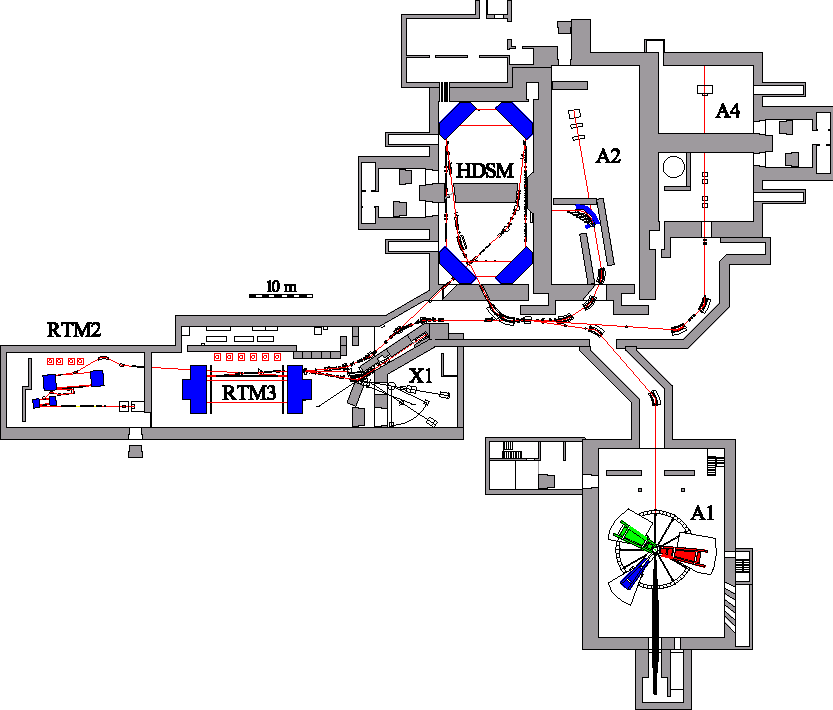
\includegraphics{grundriss}
	\caption{Grundriss der Beschleunigeranlage MAMI. Zu sehen sind die drei RTMs, der HDSM der Tagger und die verschiedenen Experimentierhallen: A1 (Elektronenstreuung), A2 (Strukturanalyse von Nukleonen), A4 (Parit\"atsverletzung) und X1 (R\"ontgenstrahlung). \cite{KPh07}}
	\label{fig.grundriss_anlage}
\end{figure}


\section{Der MAMI-Beschleuniger}
1979 wurde das MAMI erstmals in Betrieb genommen und bestand damals nur aus einem einzelnen RTM, womit eine maximale Elektronenenergie von 14 MeV erreicht werden konnte. 
Im Laufe der Jahre wurde das MAMI um zwei weitere RTMs und einem HDSM\footnote{Harmonic Double Sided Microtron} erweitert, wodurch eine Elektronenenergie von 1,5 GeV erreicht werden konnte.\cite{KPh11G} 
\newline


Um unpolarisierte Elektronen zu erzeugen, wurde eine Glühkathode auf 1000°C erhitzt. Dadurch konnten Elektronen den Heizdraht, aufgrund ihrer thermischen Bewegung, verlassen. Diese Elektronen wurden dann durch ein elektrisches Feld, welches durch die heiße Kathode und einer Anode, erzeugt wurde, zur Anode beschleunigt und traten dann durch ein Loch in der Anode aus und wurden weiter durch einen Linearbeschleuniger mit einer Frequenz von 2,45 GHz auf ca. 3,5 MeV beschleunigt. Diese Frequenz ist für das MAMI typisch und machte es zu einem Dauerstrich-Elektronen-Beschleuniger. Das heißt die Frequenz, mit der die Elektronen-Pakete auftraten, war größer, als die Frequenz, mit der die Detektoren einzelne Events auflösen konnten und somit wirkte der Strahl für die Detektoren kontinuierlich.
Am MAMI war es auch m\"oglich einen spinpolarisierten Elektronenstrahl zu erzeugen, dazu wurde ein GaAs Kristall mit polarisiertem Laserlicht bestrahlt. 

F\"ur die Experimente der A2-Kollaboration war ein unpolarisierter Strahl allerdings ausreichend.
\newline
Da die Elektronen mit einem Linearbeschleuniger nur einige MeV pro Meter beschleunigt werden k\"onnen, und man keine kilometerlangen Strecke bauen wollte, entschied man sich daf\"ur, die Elektronen mehrmals durch den gleichen Beschleunigerabschnitt zu beschleunigen. Dazu wurden sie nachdem sie beschleunigt wurden, durch zwei 180° Dipole so umgeleitet, dass sie wieder am Anfang des Beschleunigerabschnitts waren und diese Bahn abermals durchlaufen konnten. Nun besa{\ss}en die Elektronen mehr Energie und wurden in einer Bahn mit gr\"o{\ss}erem Radius durch die Dipole geleitet bis die gew\"unschte Energie erreicht wurde und der Strahl in den n\"achsten Abschnitt umgeleitet wurde. Die Struktur eines RTM erinnerte an eine antike Pferderennbahn, daher hat er auch seinen Namen.

 Eine phasengerichtete R\"uckkopplung ist allerdings nur m\"oglich, wenn die statische und die dynamische Koh\"arenzbedingung erf\"ullt sind. Um die statische Koh\"arenzbedingung zu erf\"ullen, muss die L\"ange der ersten vollst\"andigen Bahn ein ganzzahliges Vielaches der Wellenl\"ange der beschleunigten Hochfrequenz sein. F\"ur die dynamische Koh\"arenzbedingung muss die L\"angendifferenz von zwei aufeinander folgenden Uml\"aufen ebenfalls ein ganzzahliges Vielfaches der Wellenl\"ange sein\cite{Un08}. 
 
 Diese Bedingungen gaben ebenfalls die Grenzen f\"ur den maximal m\"oglichen Energiegewinn jeder Stufe an. 
\newline
Wie bereits erw\"ahnt besa{\ss} MAMI drei dieser RTMs. Die erste Stufe MAMI A bestand aus zwei RTMs mit 18 bzw. 51 Uml\"aufen. Die zweite Stufe MAMI B bestand aus dem, zu diesem Zeitpunkt, gr\"o{\ss}ten RTM der Welt mit 90 Uml\"aufen und Dipolen mit einer Breite von jeweils 5 m, wodurch sie 450 t schwer waren. Damit waren auch die technischen Grenzen erreicht.\cite{KPh11F}


\begin{figure}[h!]
	\begin{center}
	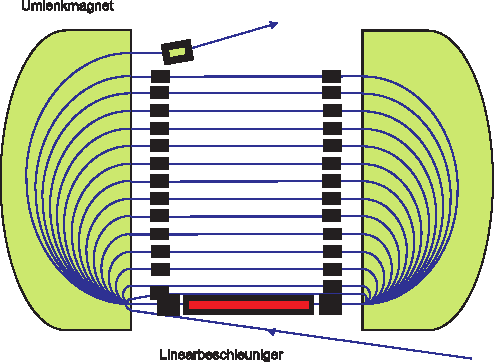
\includegraphics{RTM}	
	\caption{Prinzip eines RTM: Der Elektronenstrahl wird immer wieder durch den Linearbeschleuniger geschickt, bis die gew\"unschte Energie erreicht wurde und der Strahl mittels eines sogenannten Kicker-Magnet zum n\"achstem Abschnitt weiter geleitet wird.\cite{KPh07} }
	\label{fig.RTM}
\end{center}
\end{figure}

Damit dennoch h\"ohere Energien erreicht werden konnten, war ein neues Konzept erforderlich. MAMI C war folglich kein RTM mehr, sondern ein HDSM. Das hei{\ss}t, es bestand aus vier 90° Dipolen, welche jeweils 250 t schwer waren und einem zus\"atzlichen Linearbeschleuniger. F\"ur dieses HDSM wurde der erste Linearbeschleuniger der Welt entwickelt, der mit einer Fequenz von 4,9 GHz laufen konnte, betrieben wurde er allerdings, wie die beiden voherigen RTMs mit einer Frequenz von 2,45 GHz.
%\newline

\begin{table}[h!]
\centering


		\begin{tabular}{|l|c|c|c|c|}
			\hline
			& RTM1 & RTM2 & RTM3 & HDSM \\
			\hline
			\hline
			Eingangsenergie &3,455 MeV  &  14,35 MeV& 179,5 MeV  &854,6 MeV \\ \hline
			Ausgangsenergie &14,35 MeV  &  179,5 MeV &854,6 MeV  & 1,5 GeV \\ \hline
			Anzahl Uml\"aufe&18  &51  &90  &43 \\ \hline
			Energiegewinn pro Umlauf &0,559 MeV  & 3,24 MeV & 7,5 MeV  & 13,93-16,63 MeV \\ \hline
			
	
		\end{tabular}

		\caption{Technische Daten der MAMI-Beschleunigerstufen \cite{Un08}}
		\label{tab.MAMIstufen}

\end{table}

 Am Ende der Beschleunigung hatte der Elektronenstrahl eine Energie von ca. 1,5 GeV, diese konnte in Schritten von etwa 15 MeV eingestellt werden und sein Durchmesser lag im Mikrometerbereich, was sehr gute Voraussetzungen f\"ur Pr\"azisionsexperimente waren.\cite{KPh07}. 
 
 
 \section{Die Photonenmarkierungsanlage}
 
 In der A2-Experimentierhalle wurde schlie{\ss}lich der reelle Photonenstrahl mittels Bremsstrahlung erzeugt. Dazu traf der MAMI-Elektronenstrahl auf einen Radiator, typischerweise ein d\"unnes Metall oder ein Diamant mit einer Dicke von 10 bis 100 $\mu$m. Die Elektronen werden anschlie{\ss}end im Coloumbfeld eines Kerns des Radiators beschleunigt und k\"onnen dann, aufgrund der Impulserhaltung ein Photon in Vorw\"artsrichtung ausstrahlen.
 \begin{equation}
 e^{-}+N\rightarrow N + e^{-}+\gamma
 \label{eq.Streuung}
 \end{equation}
  Der R\"ucksto{\ss} des Kerns konnte aufgrund seiner gro{\ss}en Masse vernachl\"assigt werden und die Energie der Photonen konnte anschlie{\ss}end mit folgender Formel berechnet werden:
  \begin{equation}
  E_{\gamma}= E_{e^{}}-E_{e^-}
  \label{eq.Photonenenergie}
  \end{equation}
 Dabei war $E_e$ die Energie des Elektronenstrahls und $E_{e^-}$ die Energie der gestreuten Elektronen, welche durch den Glasgow-Mainz-Tagger (siehe Abbilding \ref{fig.TAGGER}) bestimmt wurde.
 % dieser trennt zus\"atzlich den Photonen- von dem Elektronenstrahl. Durch einen Dipol wurden die Elektronen ohne Bremsstrahlung, das hei{\ss}t ohne Energieverlust, abgelenkt und, je nach Energie, auf einen bestimmten Abschnitt des Tagger-Elektronenleiters fokussiert.  
 Dieser war ein impulsselektierendes, magnetisches Spektrometer, in dem ein magnetisches Feld angelegt war, welches die Elektronen auf Fokalebene lenkte, hinter der sich die Tagger-Elektronenleiter befand. Dadurch wurde zus\"atzlich der Elektronenstrahl von dem Photonenstrahl getrennt. Dieses Magnetfeld war zus\"atzlich so eingestellt, dass Elektronen, welche keine Energie durch Bremsstrahlung verloren haben, direkt in den Strahlenfang abgelenkt wurden. Die restlichen Elektronen wurden je nach Impuls auf einen anderen Abschnitt der Tagger-Leiter fokusiert.
 
 Diese Tagger-Elektronenleiter bestand aus 353 Szintillatoren, welche sich jeweils zur H\"alfte \"uberlappten.
 Dadurch ergaben sich 352 Kan\"ale mit einer Energieaufl\"osung von $\Delta E \approx$  2 MeV bzw. 4 MeV bei einer Strahlenenergie von $E_e=$ 800 MeV bzw. 1,5 GeV. 
 
 Folglich lie{\ss} sich der Impuls durch Kenntnis des Auftrefforts des Elektron auf der Tagger-Leiter und der St\"arke des Magnetfeldes bestimmen und dadurch auch die Energie der Elektronen.
 
 Da die Energie des Elektronenstrahls und die der gestreuten Elektronen bekannt war, konnte die Energie der Photonen mit Gleichung \ref{eq.Photonenenergie} errechnet werden.
\newline 
\begin{figure}[h!]
	\begin{center}
	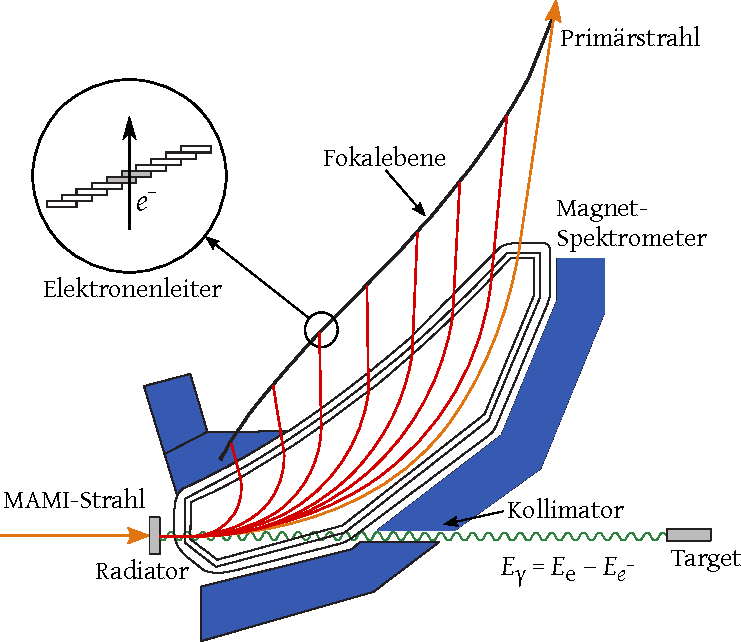
\includegraphics{TAGGER}
	
	\caption{Der Glasgow-Mainz-Tagger: Am Radiator entstanden durch Bremsstrahlung Photonen, welche den Kollimator passierten und auf das Target trafen. Die Elektronen wurden durch den Dipol auf den Elektronenleiter angelenkt, wodurch sich ihre Energie bestimmen lie{\ss}\cite{Un08}}
\label{fig.TAGGER}	
\end{center}
\end{figure}
 
\section{Das Detektorsystem}
\label{sec:Das-Detektorsystem}
Nach seiner Erzeugung traf der Photonenstrahl auf ein ca. 10 cm langes Flüssig-Wasserstoff-Target, welches sich im Zentrum des Crystal-Balls (CB) befand. Die erzeugten und gestreuten Teilchen konnten dann durch ein System von Detektoren bestehend aus dem Crystal-Ball Detektor, einem Teilchenidentifikationsdetektor (PID\footnote{Particle Ideticication Detector}), zwei Vieldrahtproportionalkammern (MWPC\footnote{Multi-Wire Proportional Chamber}) und einem Photonenspektrometer (TAPS\footnote{Two Arm  Photon Spectrometer}) nachgewiesen werden. Der PID und die MWPC waren im Inneren des CB angebracht. Der TAPS wurde am Ausgang des CB platziert, um einen fast vollständig abgedeckten Raumwinkel zu erreichen.
\begin{figure}[h!]
	\begin{center}
		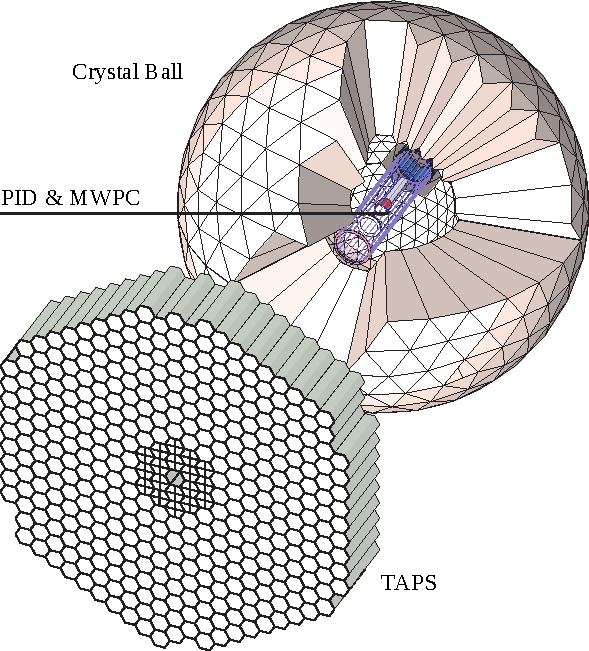
\includegraphics{crystal_ball}
	
		\caption{Anordnung des Detektorsystems: Im Zentrum des sph\"arischen Kalorimeters (CB) befanden sich der Detektor zur Teilchenidentifikation (PID) und zwei zur Bestimmung der Teilchen-Trajektorie (MWPC). Die TAPS-Wand befand sich am Ausgang des CB und sorgte daf\"ur, dass der CB einen Raumwinkel von fast 4$\pi$ abdeckte\cite{We13}}
		\label{[fig.crystal_ball]}	
\end{center}
\end{figure}

\subsection{Der Crystal-Ball-Detektor}
Ursprünglich wurde der Crystal-Ball Detektor Anfang der 70er Jahre am SPEAR\footnote{Stanford Positron Electron Asymmetric Ring} zur Entdeckung des $J/\Psi$-Mesons entwickelt. Später wurde mit seiner Hilfe das Bottom-Quark am DESY\footnote{Deutsches Elektronen-Synchrotron} und Baryonenresonanzen am BNL\footnote{Brookhaven National Laboratory} untersucht.
Seit November 2002 stand der Crystal-Ball Detektor der A2-Kollaboration am MAMI für Experimente mit reellen Photonen zur Verfügung.
\newline
Der Crystal-Ball war ein Kalorimeter bestehend aus 672 Natriumiodid (NaI) Szintillatoren, welche so angeordnet waren, dass 93,3\% des Raumwinkels abgedeckt werden konnte. Die Geometrie basierte auf der Form eines Ikosaeders, ein W\"urfel bestehend aus 20 gleichgro{\ss}en  gleichseitigen Dreiecken. Jedes dieser Dreiecke war weiter aufgeteilt in in vier kleinere gleichseitige Dreiecke, welche wiederum jeweils in neun gleichseitige Dreiecke unterteilt waren. Somit ergaben sich 720 gleichseitige Fl\"achen. Aufgrund der hohen Zahl der Fl\"achen erinnerte der Crystal-Ball an eine Hohlkugel mit einem au{\ss}en Radius von ca. 66 cm und einen Innenradius von ca. 25 cm. 

Da der Crystal-Ball Detektor urspr\"unglich in $e^+e^-$ Streuexperimenten verwendet wurde, mussten sowohl, f\"ur den Strahleneingang, als auch -ausgang 24 dieser Fl\"achen entfernt werden, wodurch insgesamt 672 Detektoren angebracht werden konnten. Die Detektoren bestanden aus NaI-Szintillatorkristallen und waren ca. 40 cm ($\sim$15,7 Strahlungsl\"angen) lang, hatten die Form eines Pyramidenstumpfes mit dreieckiger Grundfl\"ache und einer Seitenl\"ange von etwa 5 cm am schmalen und ca. 13 cm am dicken Ende. Jeder dieser Kristalle deckte etwa 0,14 \% des Raumwinkels ab und wurde durch einen eigenen Photoelektronenvervielfacher (PMT\footnote{PhotoMultiplier-Tube}) ausgelesen. 



\subsection{TAPS, PID \& MWPC}
\label{sec:TAPS-PID-MWPC}
Der PID hatte eine zylindrische Form mit einem Durchmesser von 116,5 mm und bestand aus 24 einzelnen Szintillatoren, welche jeweils 500 mm lang, 15,3 mm breit und 4 mm dick waren. Da die Szintillatoren nur eine geringe Dicke aufwiesen, verloren Photonen beim durchfliegen weniger als 1\% ihrer Energie. Geladene Teilchen auf der anderen Seite erfuhren einen Energieverlust $\Delta E$. Ihre restliche Energie wurde im Crystal-Ball abgegeben. Folglich konnte der PID zwischen geladenen und ungeladenen Teilchen unterscheiden. 

Au{\ss}erhalb des PIDs waren die MWPCs angebracht. Dabei handelte es sich um zwei, aus Anodendr\"ahten aufgebauten, Ioniastionskammern in Form von Zylindern. Die Anodendr\"ahte waren parallel zur Strahlenachse ausgerichtet und befanden sich zwischen zwei Lagen von spiralf\"ormigen Kathodenstreifen. 

Da die A2-Kollaboraions Experimente mit einem Fixed-Target untersucht und der Crystal-Ball zwei \textit{L\"ocher} f\"ur einen Strahleneingang und -ausgang besa{\ss}, wurde die TAPS-Wand entwickelt. Diese deckte einen Polarwinkel zur Strahlenachse von 1,2° bis 20° ab. Sie wurde etwa 1,5 m vom Mittelpunkt des CB entfernt positioniert und bestand aus 72 PbWO$_4$ und 366 BaF$_2$ Szintillatorkristallen. 

Somit konnte mit diesem Detektorsystem ein Raumwinkel von fast 97\% abgedeckt werden.


\chapter{Studien zur Kalibrierung des Crystal-Ball}

Zerf\"allt ein $\pi^0$, so werden nach Reaktion \ref{eq.pi0decay} zwei Photonen frei. Diese Photonen wurden durch den Crystal-Ball Detektor nachgewiesen. Dabei wurde sowohl der Winkel zwischen den beiden Photonen, als auch die Energie der Photonen bestimmt, um die invariante Masse des $\pi^0$ ausrechnen zu k\"onnen.

Zur Analyse wurde ANT\footnote{Analysis Toolkit} benutzt. Mit diesem Programm konnten auch alle gew\"unschten Bedingungen eingestellt werden. 

\section{Reelle Daten}\
\label{sec:Reelle-Daten}

Im folgenden Abschnitt werden die gemessenen Daten aus der Strahlzeit Oktober 2014 verwendet.

\subsection{Energie-Interval Abhängigkeit}
\label{sec:Energie-Interval-Abhaengigkeit}

Als erstes wurde überprüft, ob es eine Abhängigkeit der Kalibrierung im Bereich verschiedener Energieintervalle gab. Sprich, stimmt die Kalibrierung auch dann noch, wenn die Energie der beiden detektierten Photonen sich ähnelte. Das hei{\ss}t, die Differenz der Energie der beiden Photonen betr\"agt maximal 25 MeV. Diese Bedingung wurde eingef\"uhrt, da man auf diese Weise herausfinden konnte, ob die Kalibirierung auch noch f\"ur zum Beispiel hoch energetische Photonen stimmt, da man wei{\ss}, dass beide Photonen eine hohe Energie besa{\ss}en. Anders konnte sonst nicht die Folgerung getroffen werden, da man sonst eine '\textit{Mischung}' der Energien hat und man nicht sagen kann, welcher Effekt durch welche Energie verursacht wurde.

Zur Untersuchung konnten dann aus den Daten der Strahlzeit, die invariante Masse des $\pi^0$ mit folgender Gleichung berechnet werden.

 \begin{equation}
 \begin{split}
 {m_{\pi^0}=\sqrt{2E_1E_2(1-cos(\vartheta))}}
 \label{eq:Formel-zur-Berechnung-der-invarianten-Masse}
 \end{split}
 \end{equation}

Hier ist $m_{\pi^0}$ die berechnete Masse aus den beiden Energien $E_1$ und $E_2$ der Photonen. $\vartheta$ ist der Winkel zwischen den beiden Photonen. Um diesen zu berechnen musste angenommen werden, dass das Pion im Ursprung zerf\"allt. Mehr dazu in Kapitel \ref{sec:Z-Vertex-Abaengigkeit}.
Die Herleitung der Gleichung \ref{eq:Formel-zur-Berechnung-der-invarianten-Masse} befindet sich im Anhang \ref{sec:Herleitung-der-Formel-zur-Berechnung-der-invarianten-Masse}.

Mit diesen Daten konnte schließlich ein zweidimensionales Histogramm mit der invarianten Masse auf der x-Achse angelegt werden. Auf der y-Achse wurde die Energie der Photonen aufgetragen, welche in Intervalle mit einer Breite von 25 MeV unterteilt wurden. 


\begin{figure}[h!]
	\begin{center}
		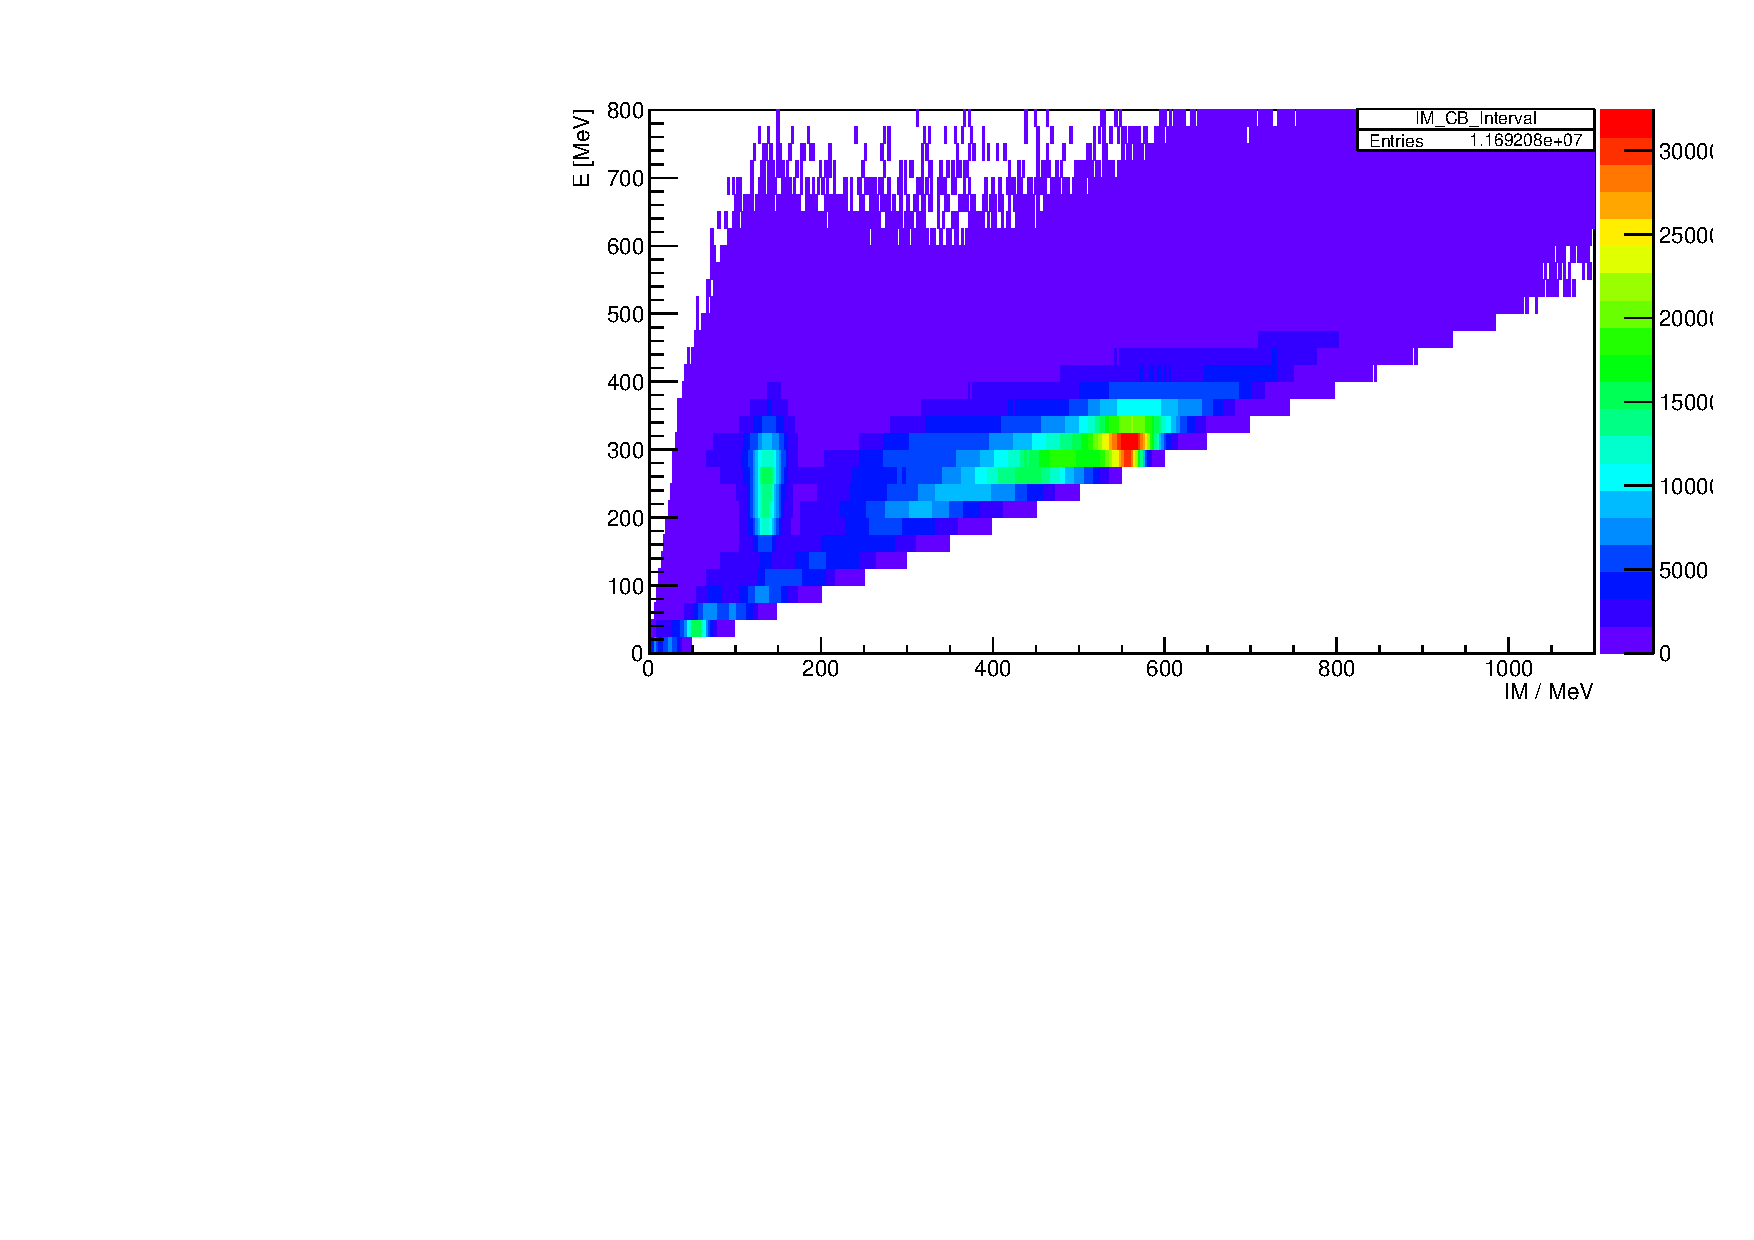
\includegraphics[width=100mm]{20172803IM_CB_Symmetric}
	
		\caption{2-D Histogramm: Auf der x-Achse ist die errechnete invariante Masse aufgetragen, die y-Achse ist in 25 MeV Intervalle aufgeteilt. Es wurden nur dann die Invariante Masse errechnet, wenn die Energiedifferenz der beiden Photonen kleiner als 25 MeV war.}
			\label{fig:Energy-Interval-Hist-All-Bins}
	\end{center}
\end{figure}

Beim Füllen des Histogramms wurde darauf geachtet, dass sich die Energien der beiden Photonen um maximal 25 MeV unterschieden.

Im folgenden wurden nur die Energieintervalle f\"ur Photonen von 125 MeV bis 425 MeV ber\"ucksichtigt.
Dieser Bereich wurde bewusst gew\"ahlt, da f\"ur kleinere Energien der Peak des $\pi^0$ zu stark durch das Rauschen gest\"ort wurde und somit die Position nicht eindeutig bestimmt werden konnte. F\"ur Energien oberhalb von 425 MeV lagen nicht mehr genug Ereignisse vor, sodass h\"ohere Energieintervalle ebenfalls verworfen werden mussten. 


Um nun die Position des $\pi^0$ zu bestimmen, wurde für jedes Intervall über den Bereich der errechneten invarianten Masse von 50 MeV bis 220 MeV mit Hilfe von ROOT gefittet. Die Einschr\"ankung des Bereichs erm\"oglichte einen besseren Fit.



 Zum Fitten wurde zun\"anchst auf ein bereits existierendes Fitmodul zur\"uckgegriffen. Dieses war eine Kombination aus einer Gau{\ss}funktion und einer Potenzreihe. Allerdings entspricht die Form des Peaks nicht der einer Gau{\ss}verteilung, weswegen eine alternative Fitfunktion gesucht werden musste. 
 
 Bei dieser neuen Funktion handelte es sich um die Crystal-Ball-Funktion, welche nach der Crystal-Ball Kollaboration benannt wurde. Diese Funktion war eine Dichtefunktion einer asymmetrischen Wahrscheinlichkeitsverteilung und war in zwei Bereiche aufgeteilt. Im zentralen Bereich entsprach sie einer Gau{\ss}form, diese ging f\"ur kleine Werte in eine Potenzreihe \"uber.
 
 \begin{equation}
 f(x|\alpha,n,\bar{x},\sigma)=N\begin{cases}exp(-\frac{(x-\bar{x})^2}{2\sigma^2}), \textnormal{  falls $\frac{x-\bar{x}}{\sigma}> -\alpha$} \\
 A(B-\frac{x-\bar{x}}{\sigma})^{-n}, \textnormal{  falls $\frac{x-\bar{x}}{\sigma}\leqslant -\alpha$} 
 \end{cases}
 \label{eq:Crystal-Ball-Funktion}
 \end{equation}
 
 Dabei war $N$ der Normierungsfaktor, $\bar{x}$ der Erwartungswert und $\sigma$ die Standardabweichung der Gau{\ss}funktion. Der Parameter $\alpha$ gab die Position an, an dem die Gau{\ss}verteilung in das Potenzgesetz, mit dem freien Parameter $n$, \"ubergeht\cite{NBI15}. 
 
 ROOT stellte diese Funktion bereits gr\"o{\ss}tenteils zur Verf\"ugung, lediglich die Normierung musste noch nachtr\"aglich hinzugef\"ugt werden.
 
 Der Untergrund wurde weiterhin mit einem Polynom vierten Grades angen\"ahert, bevor die Crystal-Ball-Funktion angewand wurde.
 
 \begin{figure}[h!]
 	\begin{center}
 		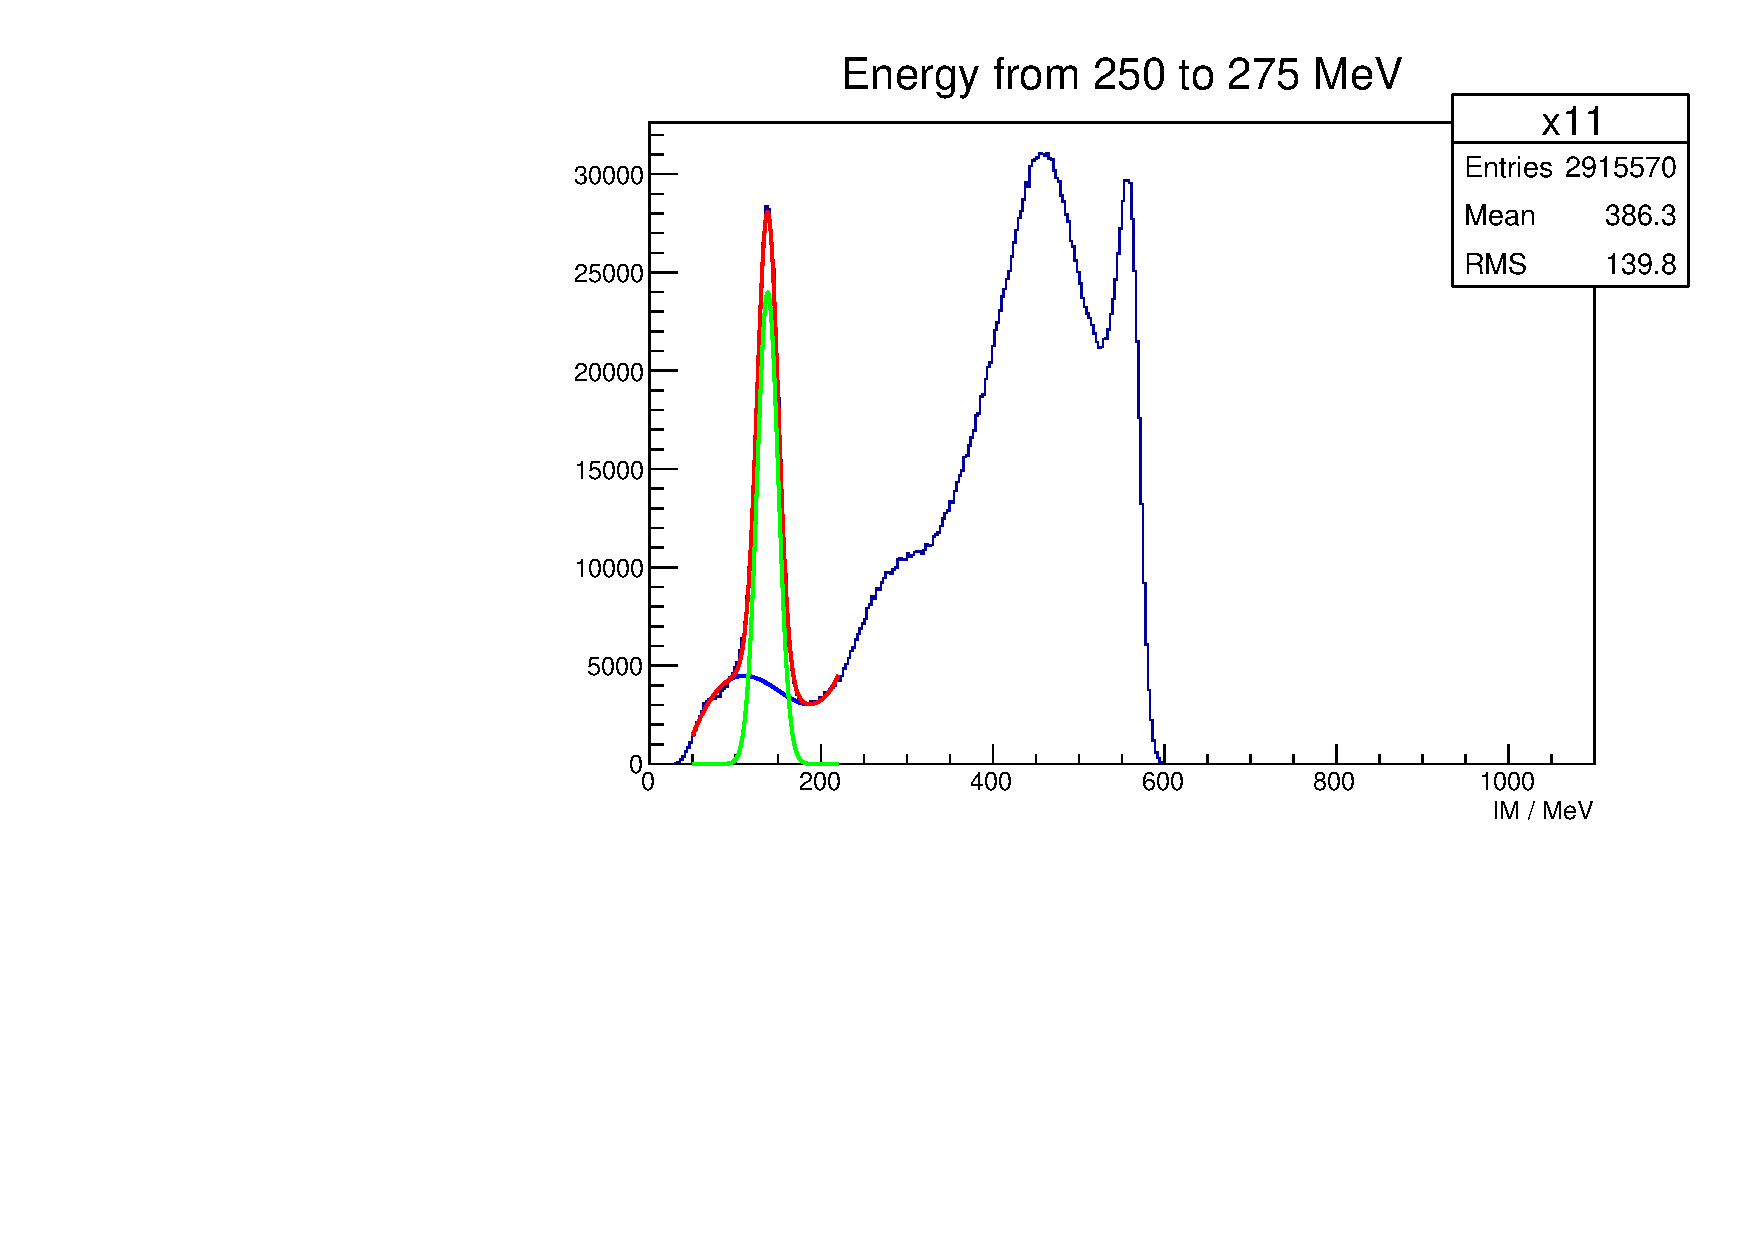
\includegraphics[width=100mm]{20172803SynnetricCBFFitExample}
 		
 		\caption{Beispiel eines Fits. Es handelt sich dabei um das Energieintervall von 250 MeV bis 275 MeV mit der Bedingung, dass sich die Energie der Photonen im gleichem Intervall befanden.
 			Zu erkennen ist der Untergrundfit (Blau), der Crystal-Ball-Fit (Gr\"un) und die Addition der beiden Fits (Rot). Alle weiteren Fits mit dieser Bedingung sind in Abbildung \ref{fig:similarenergyallfits} zu sehen.
 		}
 		\label{fig:fitexampleenergyinterval0903}	
 	\end{center}
 \end{figure}
 
  Zuerst wurde der Untergrund mit einem Polynom vierten Grades gefittet, in Abbildung \ref{fig:fitexampleenergyinterval0903} blau dargestellt. Von den Daten konnte damit der Untergrund abgezogen werden. Nun wurde \"uber die verbleibenden Daten der Crystal-Ball-Fit angewand (Gr\"un). Damit leichter \"uberpr\"uft werden konnte, ob der Fit sinnvoll war, wurde beide Fits addiert und zus\"atzlich in den Graphen gezeichnet (Rot). In dieser Abbildung  und in Abbildung \ref{fig:Energy-Interval-Hist-All-Bins} ist ebenfalls das $\eta$-Meson bei einer Masse von ungef\"ahr 550 MeV zu erkennen. Sein Peak wird allerdings sehr stark durch den Untergrund gest\"ort. Der Fokus dieser Arbeit lag zwar bei der Betrachtung des $\pi^0$, allerdings war es auch interresant die Position des $\eta$-Peaks zu betrachten, daher wurde nach einem Weg gesucht, den Untergrund m\"oglichst stark zu reduzieren. 
  
 Daher wurde nun auch \"uberpr\"uft, ob die detektierten Teilchen eine Ladung besa{\ss}en, wenn ja, dann handelte es sich nicht um Photonen und sie wurden nicht in das Histogramm eingef\"ugt. 
 
\begin{figure}[h!]
\centering
\begin{minipage}{0.45\textwidth}
	\centering
		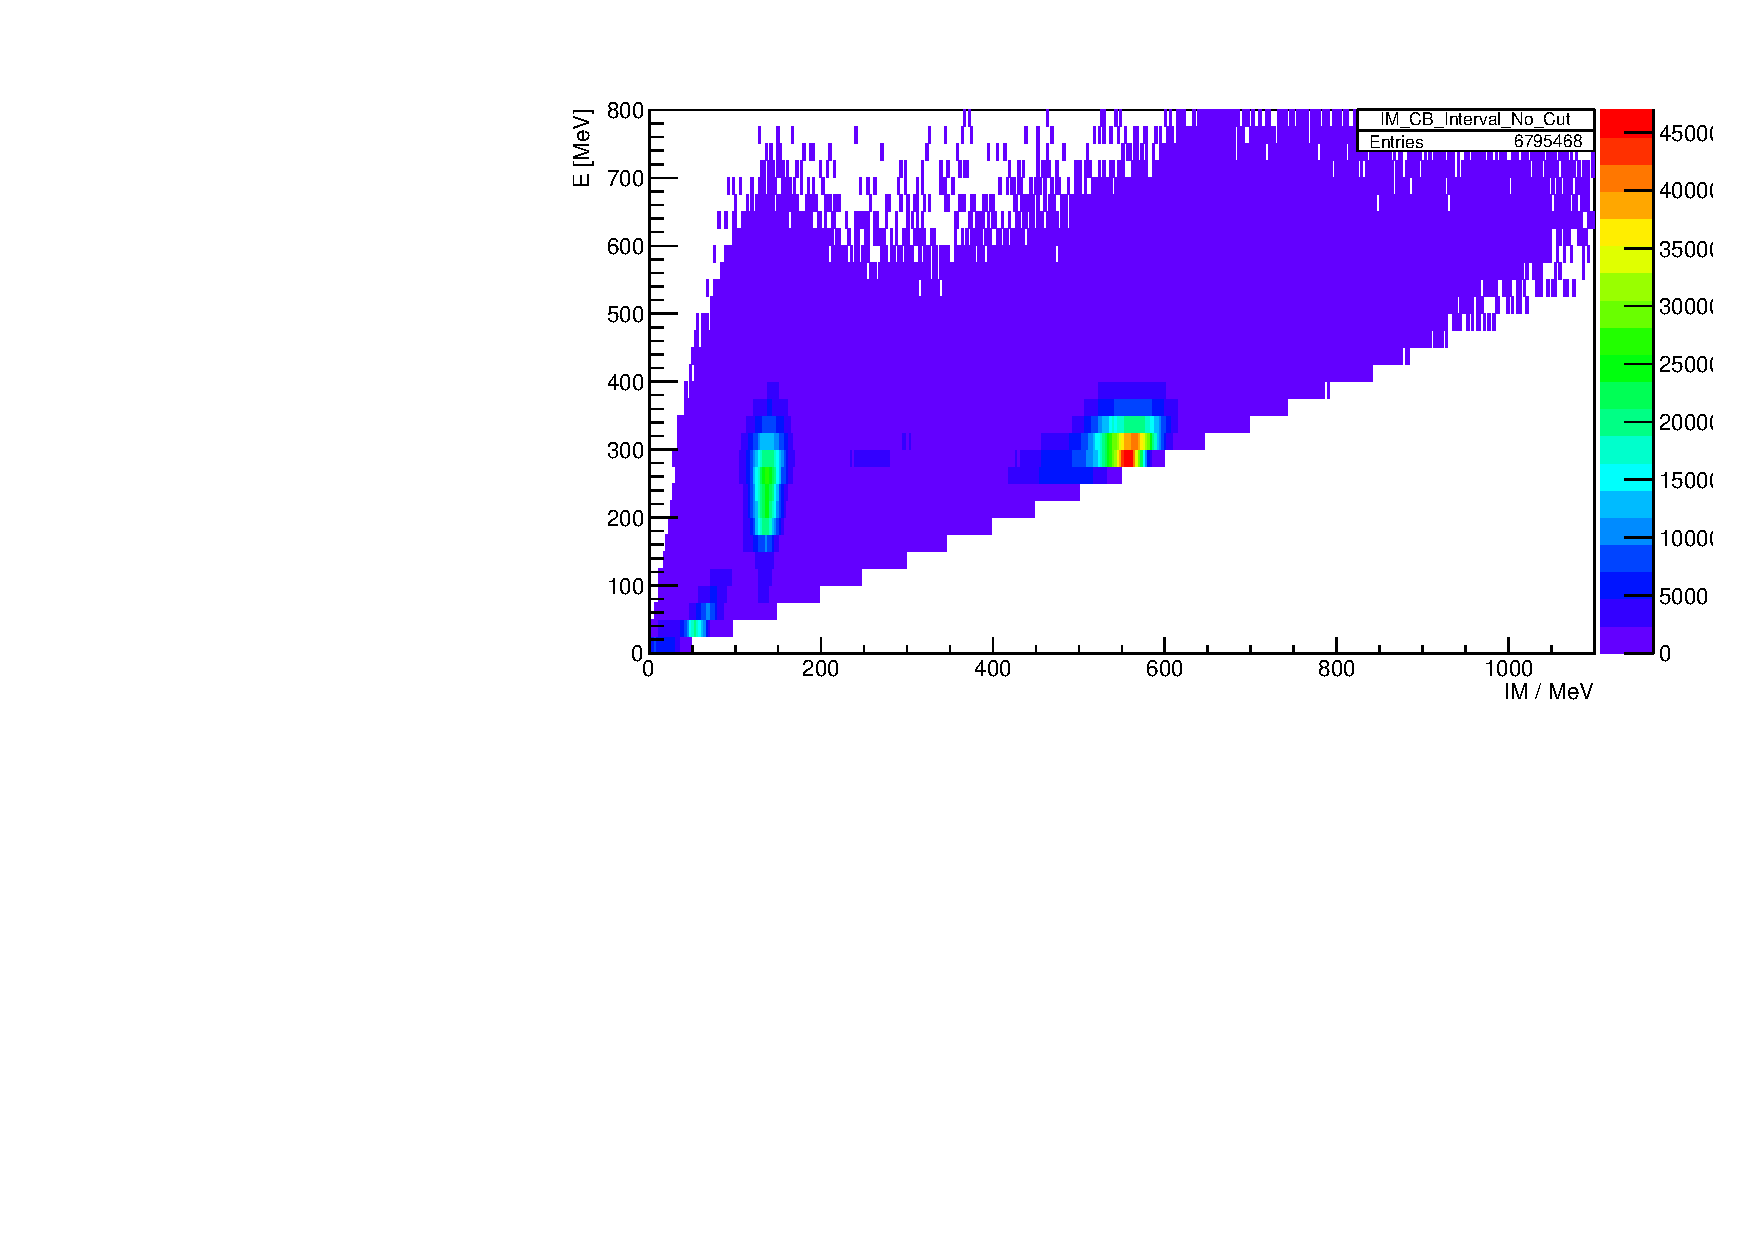
\includegraphics[width=0.9\textwidth]{20172803IM_CB_Uncharged_Symmetric_No_Cut}
		
		\label{fig:Symmetric-Uncharged-Hist-No-Cut}
\end{minipage}
\hfill
\begin{minipage}{0.45\textwidth}
	\centering
	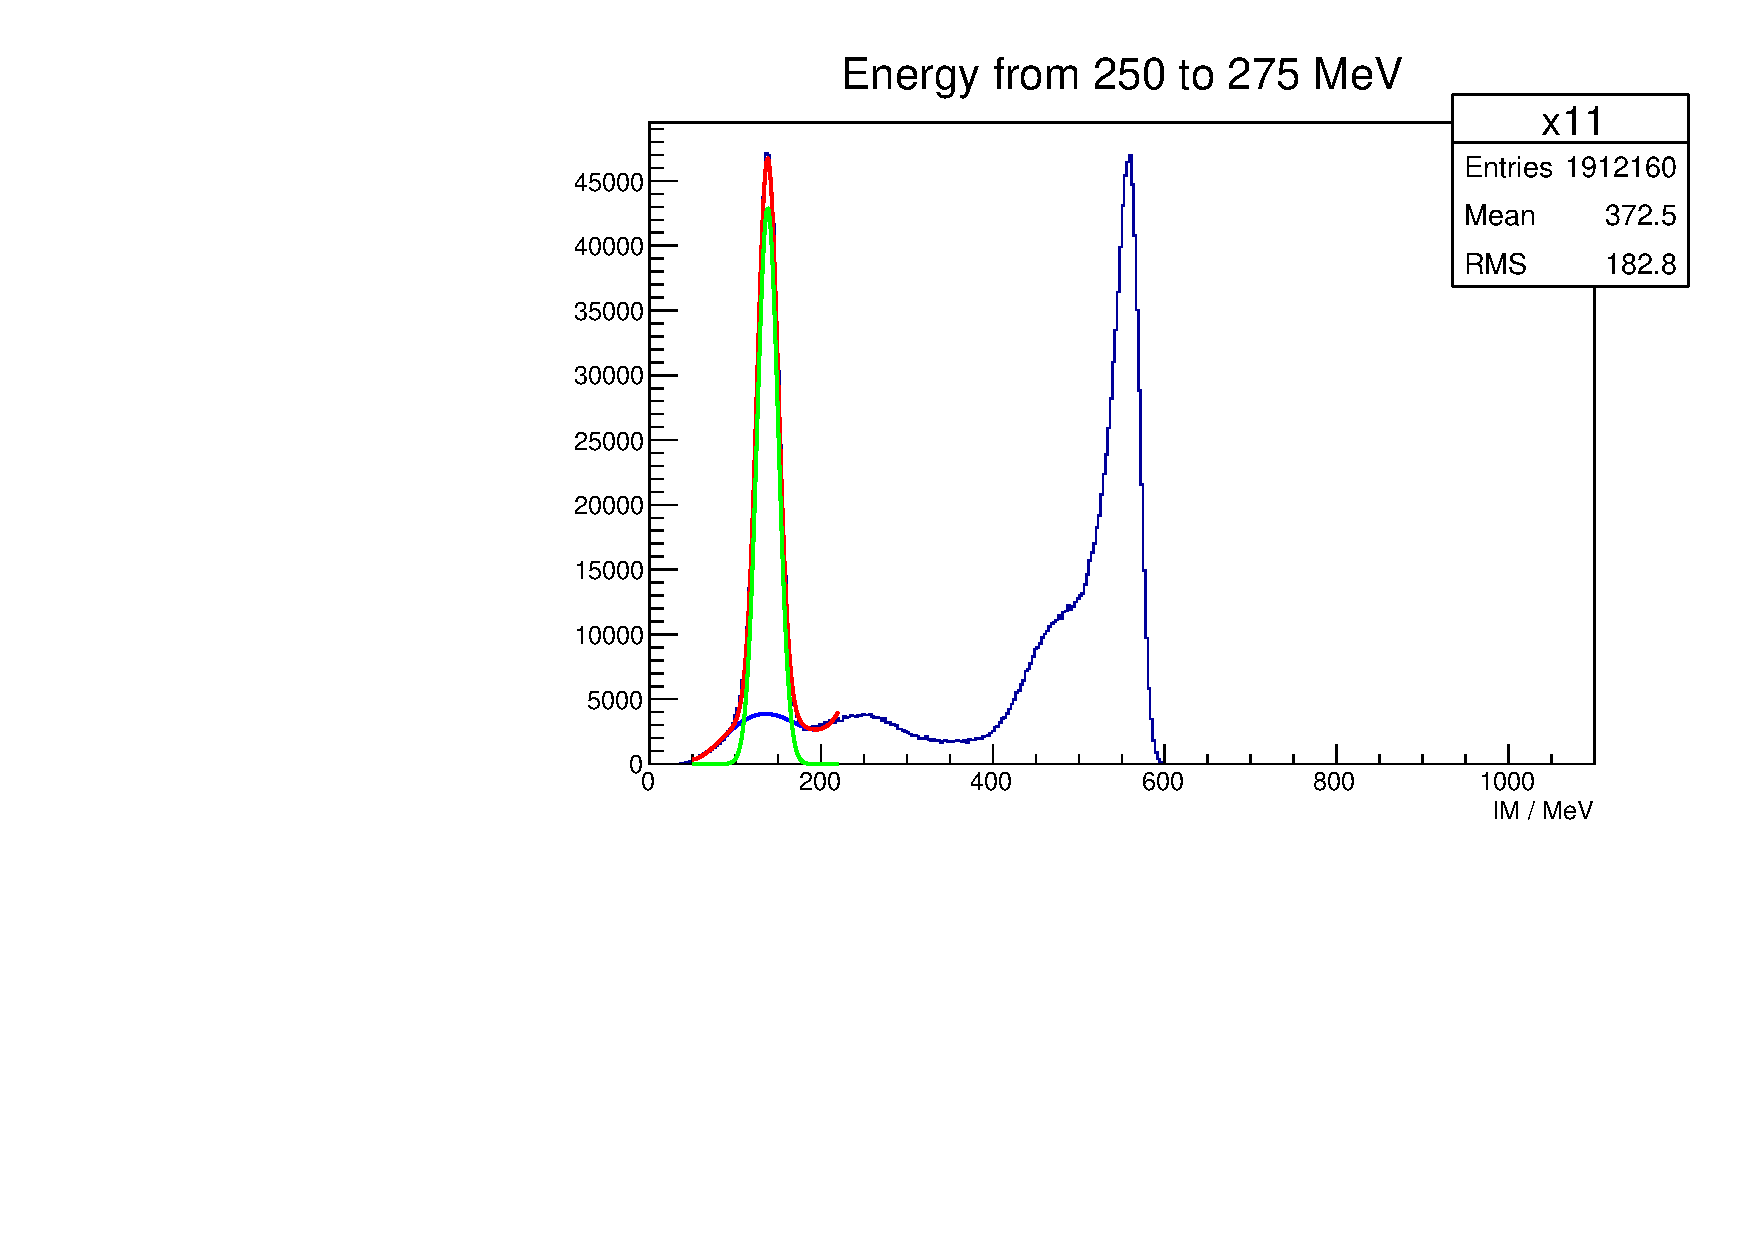
\includegraphics[width=0.9\textwidth]{20172803SymmetricUnchargedCBFFitExample}
\end{minipage}
\caption{Links ist das 2-D Histogramm zu sehen, f\"ur welches \"uberpr\"uft wurde, ob die gemessenen Teilchen ungelafen waren. Rechts ist ein Beispielfit aus diesem Historgramm mit der Crystal-Ball-Funktion zu sehen. Sowohl der $\pi^0$, als auch der $\eta$-Peak sind deutlich ausgepr\"agter.}
\end{figure}
 
 Bereits an diesem neuem Histogramm war zu erkennen, dass die St\"orung durch den Untergrund stark reduziert wurde, was einen besseren Fit f\"ur sowohl das $\pi^0$ als auch das $\eta$ erm\"oglichte.
 
 Nun wurde auch \"uber dieses Histogramm f\"ur das $\pi^0$ von 125 MeV bis 425 MeV gefittet.
 Aus diesen Fitdaten konnte dann die Position des $\pi^0$ bestimmt werden. 
 
 \begin{figure}[h!]
 	\begin{center}
 		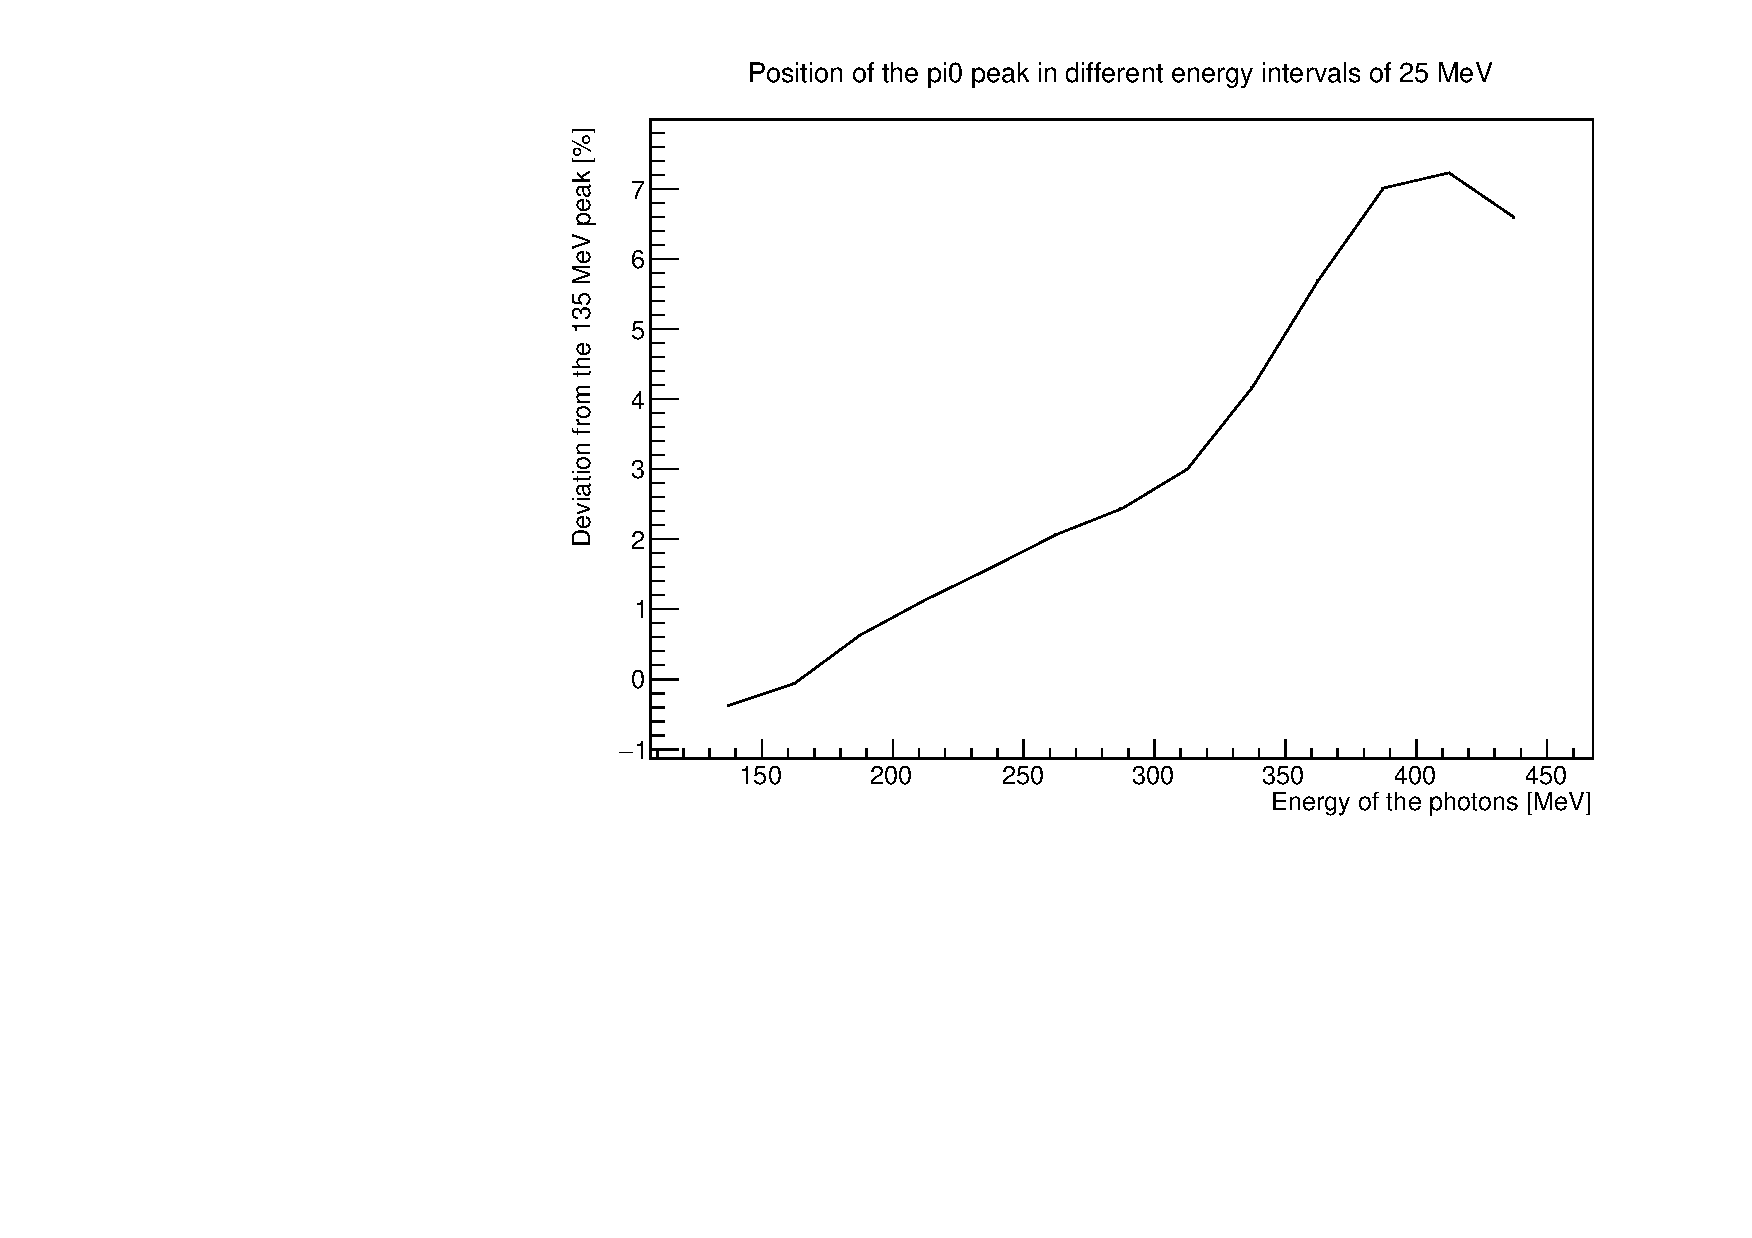
\includegraphics[width=100mm]{20172803SymmetricUnchargedDeviation}
 	
 		\caption{Die errechnete Position des $\pi^0$ Peaks wurde gegen die Energie der Photonen aufgetragen.
 			Es galt die Bedingung, dass die gemessenen Teilchen ungeladen sein mussten und dass die Energie der Photonen sich \"ahneln sollte.
 			%
 		} 
 		\label{fig.Energydependency_pion}
 	\end{center}
 \end{figure}

In Abbildung \ref{fig.Energydependency_pion} wurden die errechneten Positionen der Pionen gegen die Energie der Photonen aufgetragen. Zu sehen ist eine deutliche Abweichung zum Literaturwert des $\pi^0$ Peaks. Auch nahm die Abweichung für größere Energien zu und betrug teilweise \"uber 7\%. Zus\"atzlich f\"allt auf, dass die errechnete invariante Masse fast ausschlie{\ss}lich gr\"o{\ss}er als erwartet war.
  
Daraus folgte, dass eine Abhängigkeit zwischen der Position des $\pi^0$-Peaks und der Energie der Photonen vorlag. Die Ursache dieser Abh\"angigkeit soll in den Folgenden Abschnitten bestimmt werden.

%Daraufhin wurde das gleiche Verfahren nochmal angewendet, allerdings wurde dieses mal die Bedingung weggelassen, dass die Photonen sich energetisch ähneln mussten. Die Bedingung, dass die registrierten Teilchen ladungsfrei sein mussten, galt weiterhin. Die errechnete invariante Masse der Photonen wurde in das Histogramm (Abb.: \ref{fig:Energy-Intervall-Hist-All-Energys-No-Condition}) eingetragen. Die Energieintervalle wurden direkt mit der Crystal-Ball-Funktion gefittet. Zu sehen in Abbildung \ref{fig:allenergyallfits}. Nun wurden ebenfalls die errechneten invarianten Massen des $\pi^0$ gegen die Energien der Photonen aufgetragen (Abb.: \ref{fig:Energy-Intervall-No-Condition-Deviation-1303}). Auch hier war eine deutliche Abweichung der Position des $\pi^0$ zum Literaturwert zu erkennen. Diese Abweichungen betrugen zwar nur fast 2\% (siehe Abb. \ref{fig:Relative-Deviation-Energy-Interval-No-Condition}}), sind aber nicht vernachl\"assigbar. 




\subsection{Vernachl\"assigung der Detektoren am Rand}
\label{sec:Vernachlaessigung-der-Detektoren-am-Rand}

Als Ursprung der in Kapitel \ref{sec:Energie-Interval-Abhaengigkeit} ermittelten Abweichung wurde zun\"achst der Aufbau des Crystal-Balls vermutet. Genauer gesagt, der Strahlenein und -ausgang. Denn durch diese hatten die Detektoren im Crystal-Ball nicht alle gleich viele Nachbar Detektoren und da ein Photon seine gesamte Energie nicht an einen Detektorkristall abgab, sondern immer auch an seine Nachbarn, konnten diese Randdetektoren nicht ideal kalibriert werden. 


%In erster Linie war es wichtig einen Vergleich zwischen der $\pi^0$ Position mit und ohne Ber\"ucksichtigung der Detektoren am Rand zu erhalten. Es sollte herausgefunden werden, ob so die Messung verbessert werden konnte. Zus\"atzlich galten, wie in Kapitel \ref{sec:Energie-Interval-Abhaengigkeit}, die Bedingungen, dass die Energie der Photonen sich im gleichem Energieinterval befand und dass die registrierten Teilchen ungeladen sein m\"ussen. 
%ohne die Bedingung, dass die Histogramme nur gef\"ullt werden d\"urfen, wenn sich die Energie der Photonen im gleichem Intervall befand. 

%\begin{figure}[h!]
%	\begin{center}
%		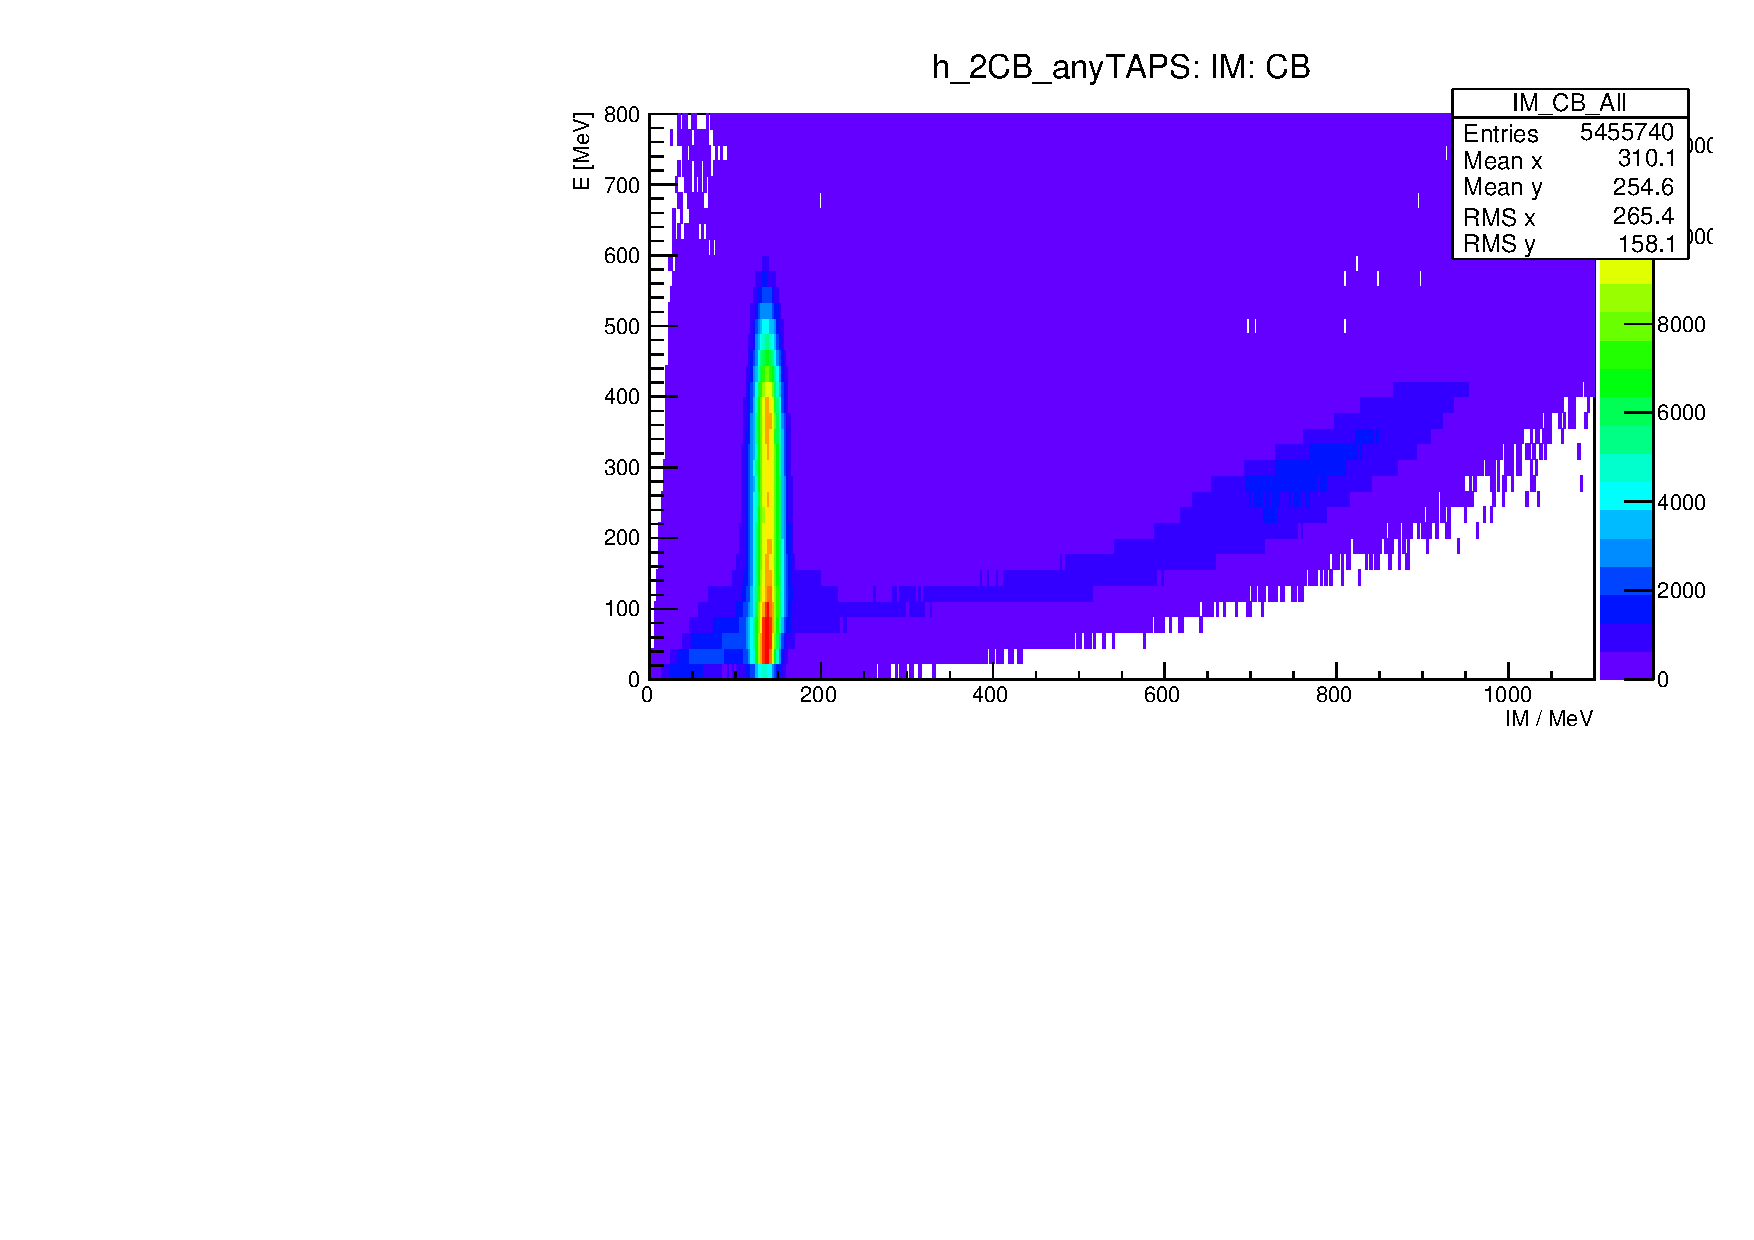
\includegraphics[width=100mm]{EnergyAngle2DHistoNoEdgePi0Position1403}
%		\caption{2-D Histogramm: Auf der x-Achse ist die errechnete invariante Masse und auf der y-Achse ist der Energie der Photonen aufgetragen. Die y-Achse ist in Energieintervalle der Breite 25 MeV unterteilt}
%		\label{fig:2D-Hist-Angle-Energy-Position-Pi0}
%	\end{center}
%\end{figure}

%Das gef\"ullte Histogramm ist in Abbildung \ref{fig:2D-Hist-Angle-Energy-Position-Pi0} zu sehen. Hier erkennt man auch direkt, dass simulierte Daten benutzt wurden, da der $\pi^0$-Peak viel st\"arker ausgepr\"agt war, im Vergleich zu den reellen Daten.

Zus\"atzlich zu den in Kapitel \ref{sec:Energie-Interval-Abhaengigkeit} geltenden Bedingungen wurde noch die Bedingung hinzugef\"ugt, dass die Detektoren am Rand des Strahlenein- und ausgangs nicht betrachtet wurden. Dies erreichte man dadurch, dass alle Reaktionen, die ein oder mehrere Photonen besa{\ss}en, welche einen Winkel von 30° oder weniger zur Strahlenachse hatten, verworfen wurden. Diese Gradzahl wurde durch eine Absch\"atzung errechnet. Die \"Offnungen f\"ur den Strahlenein- und ausgang hatten einen '\textit{Radius}' von 2 Detektoren, und erstreckte sich \"uber einen Polarwinkel von 20°. Folglich h\"atte ein Ring aus Detektoren um diese \"Offnungen einen Polarwinkel von 10°. 
 
Auch f\"ur diese Bedingung wurde anschlie{\ss}end ein Histogramm angelegt (Abb.: \ref{fig:30-Degree-Cut-Histogramm}) und die einzelnen Positionen wurden dann gefittet (Abb.: \ref{fig:30-Degree-Cut-RealData-All-Fits}), um die Position des $\pi^0$ zu bestimmen. Das Energieintervall das betrachtet und gefittet wurde entsprach dem aus Kapitel \ref{sec:Energie-Interval-Abhaengigkeit}, damit ein war ein besserer Vergleich zwischen den verschiedenen Effekte m\"oglich.

\begin{figure}[h!]
	\begin{center}
		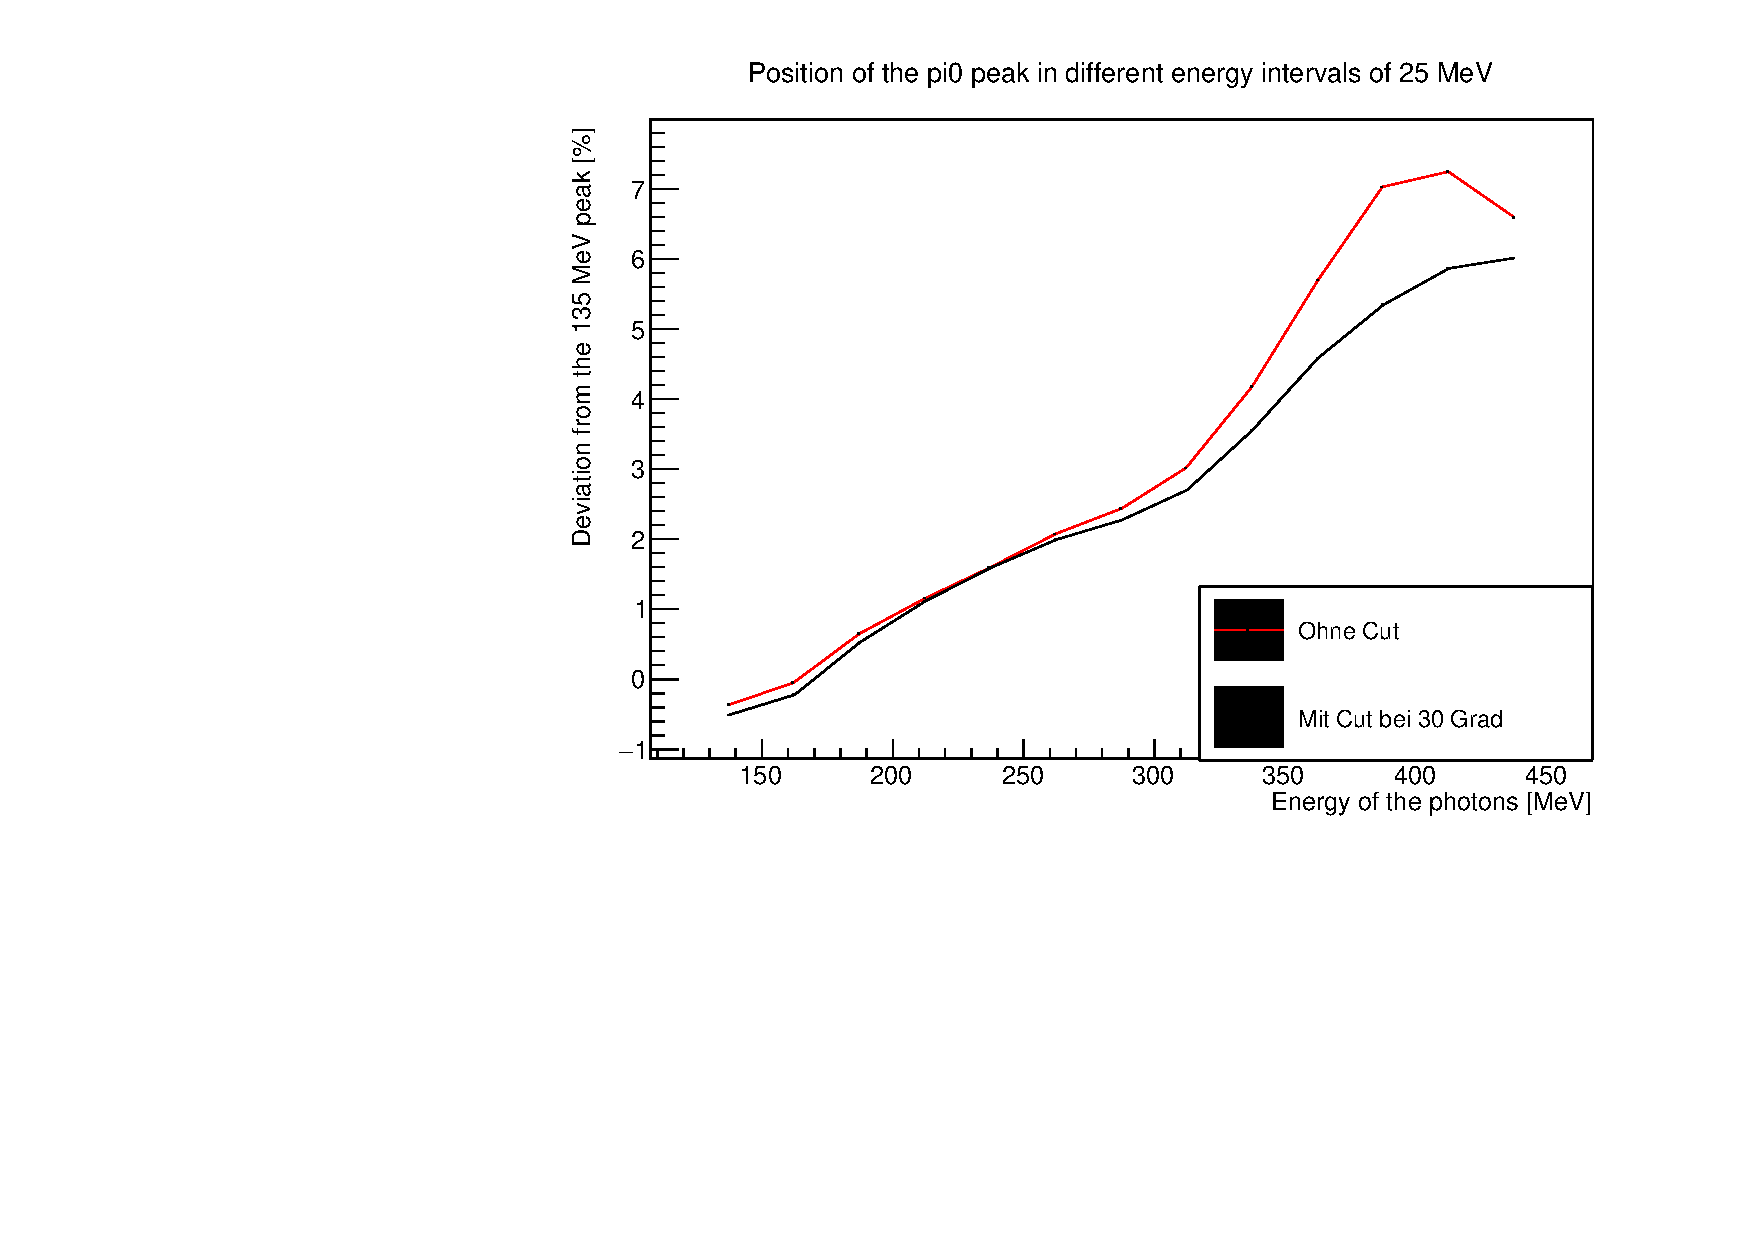
\includegraphics[width=100mm]{20172803SymmetricUnchargedDeviationCut}
		\caption{Die relative Abweichung wurde in Prozent gegen die Energie der Photonen gezeichnet. Die rote Linie stellt die relative Abweichung ohne die Bedingung, dass Photonen mit einem Winkel kleiner als 30° verworfen wurden, die schwarze Linie mit der Bedingung.}
	\end{center}
\end{figure}

Zum besseren Vergleich der beiden Ergebnisse wurden die relative Abweichungen mit und ohne Bedingung zusammen in einen Graphen gezeichnet. 

In diesem erkennt man, dass der Unterschied f\"ur Photonenenergien unterhalb von 275 MeV nur sehr klein ist und weniger als 0,1\% betr\"agt. Bei einem so kleinen Unterschied kann man nicht mit Gewissheit sagen, dass der Cut bei 30° eine Verbesserung der $\pi^0$-Peak Position bewirkt hat. Die Differenz ist noch im Bereich der statistischen Fluktuation. 

F\"ur Photonenenergien oberhalb von ca. 275 MeV nimmt diese Abweichung jedoch zu und betr\"agt teilweise \"uber 1\%.

Ein Grund daf\"ur war, dass hochenergetische Photonen dann erzeugt werden, wenn auch das Pion eine hohe kinetische Energie besa{\ss}. Diese Photonen haben dann eine gr\"{ss}ere Wahrscheinlichkeit in Richtung des Strahlenausgang des Crystal-Balls aufzutreten.

Um das zu erkl\"aren betrachte man zun\"achst ein ruhendes $\pi^0$. Dieses zerf\"allt in 2 Photonen in zuf\"alliger Richtung mit einem Winkel von 180° zueinander und mit einer Energie von jeweils etwa 67,5 MeV. 

Gibt man dem $\pi^0$ nun einen Boost in z-Richtung, so erhalten auch die beiden Photonen einen Boost in diese Richtung.
Zur Veranschaulichung betrachte man nun zwei extrem Beispiele:

\begin{enumerate}
	\item Im Ruhesystem des $\pi^0$ werden die Photonen in einem Winkel von 90° zur Strahlenachse ausgesandt. Wird nun ein Boost in z-Richtung angewandt, so erhalten beide Photonen einen gleich gro{\ss}en Impuls in z-Richtung und haben folglich beide die gleiche Energie und den gleichen Winkel zur z-Achse.
	\item Werden die Photonen allerdings entlang der z-Achse ausgesandt. Ein Boost in z-Richtung bewirkt nun, dass das Photon in z-Richtung Energie dazu erh\"alt, w\"ahrend das Photon entgegengesetzt zur z-Richtung Energie '\textit{verliert}'. Die Energiedifferenz nimmt also zu.
\end{enumerate}

F\"ur h\"ohere Energien werden diese Effekte verst\"arkt und alles in allem werden mehr Photonen in Strahlenrichtung gemessen. Daraus folgt, dass Photonen mit niedrieger Energie sich eher gleichm\"a{\ss}ig im Raum verteilen, w\"ahrend hochenergetische Photonen h\"aufiger am Strahlenausgang des Crystal-Balls auftreten.

Dies f\"uhrte auch zu einem weiteren Problem. Dadurch, dass die h\"oher energetischen Photonen wahrscheinlicher am Strahlenausgang vorliegen, werden nicht alle Detektoren im Crystal-Ball gleich ber\"ucksichtigt. So liegen, am Strahleneingang fast keine hochenergetische Photonen vor.


\begin{figure}[h!]
	\centering
	\begin{minipage}{0.45\textwidth}
		\centering
		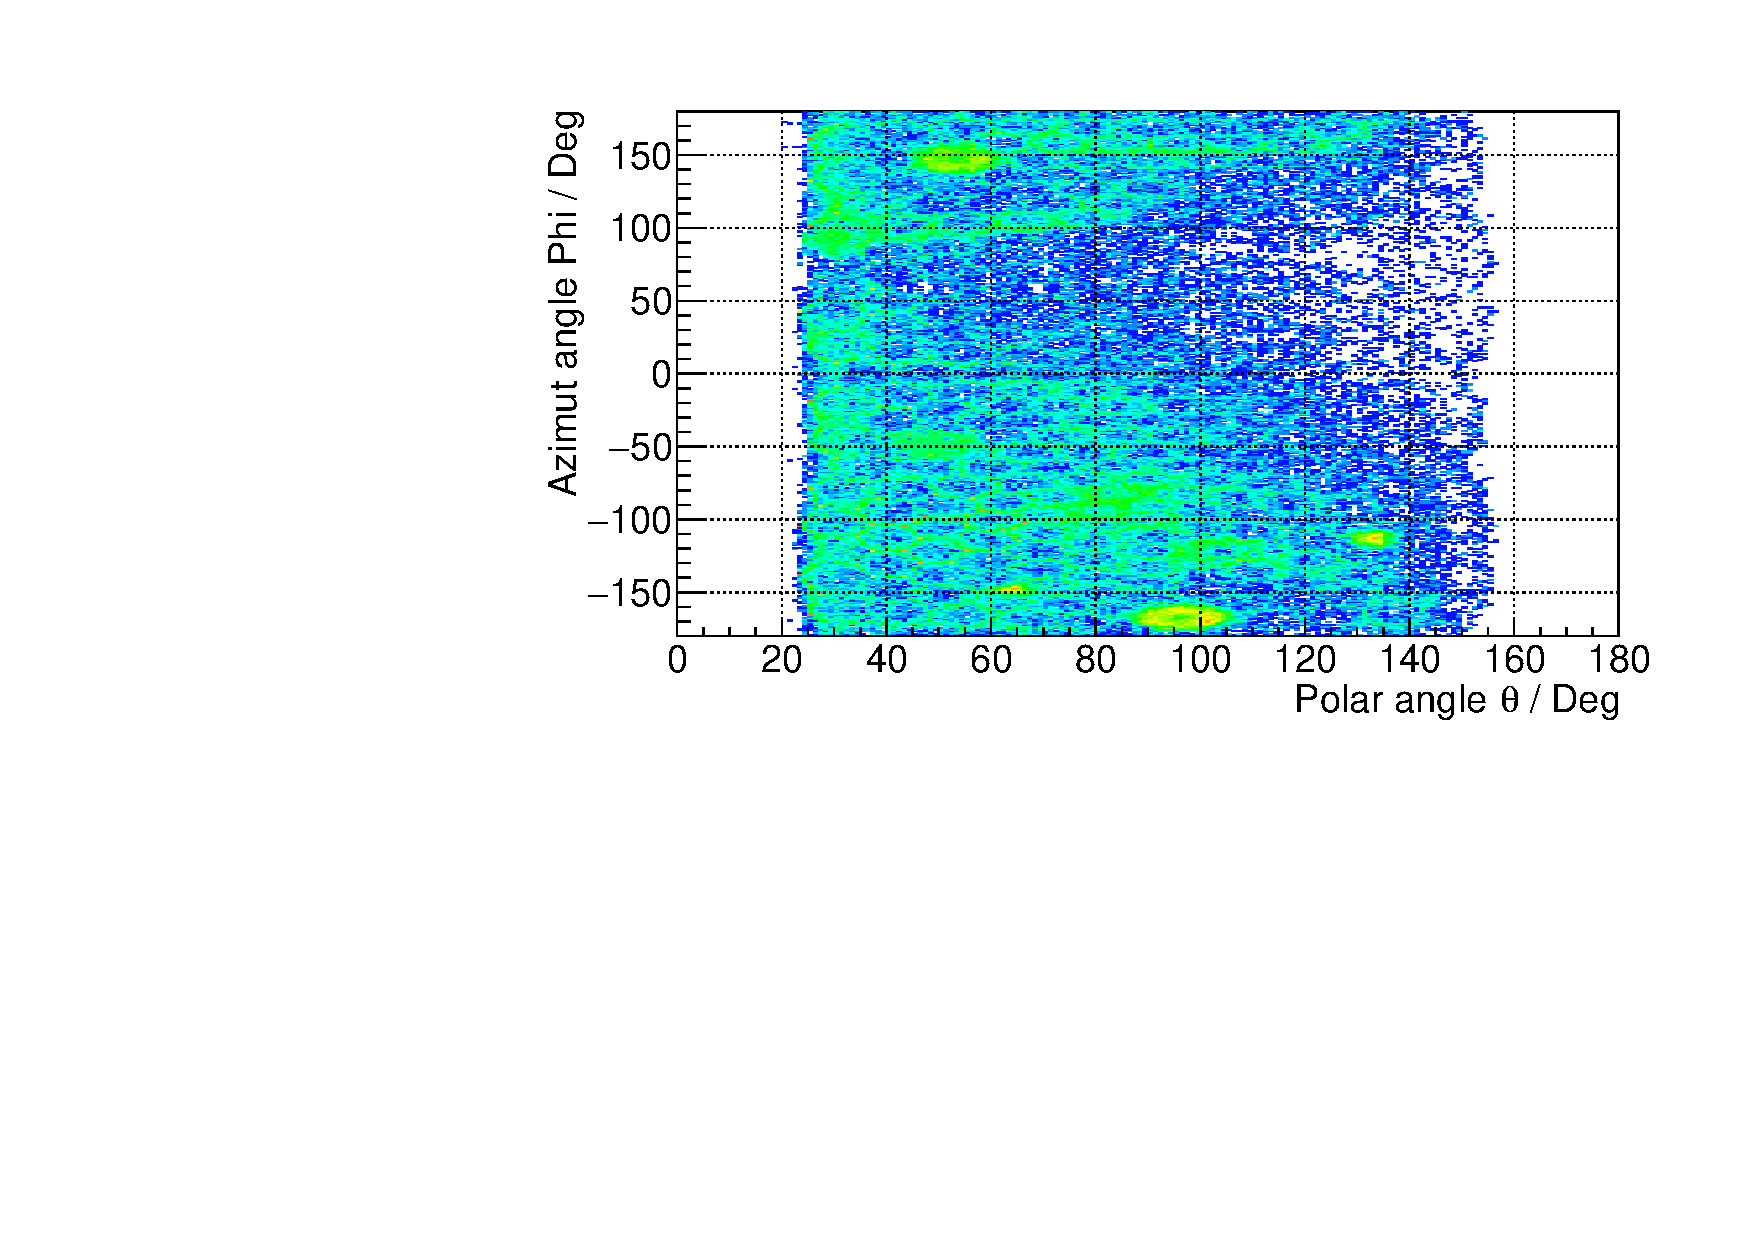
\includegraphics[width=0.9\textwidth]{20170504ThetaPhiEnergySymmetric2014_10_125}
	\end{minipage}
	\hfill
	\begin{minipage}{0.45\textwidth}
		\centering
		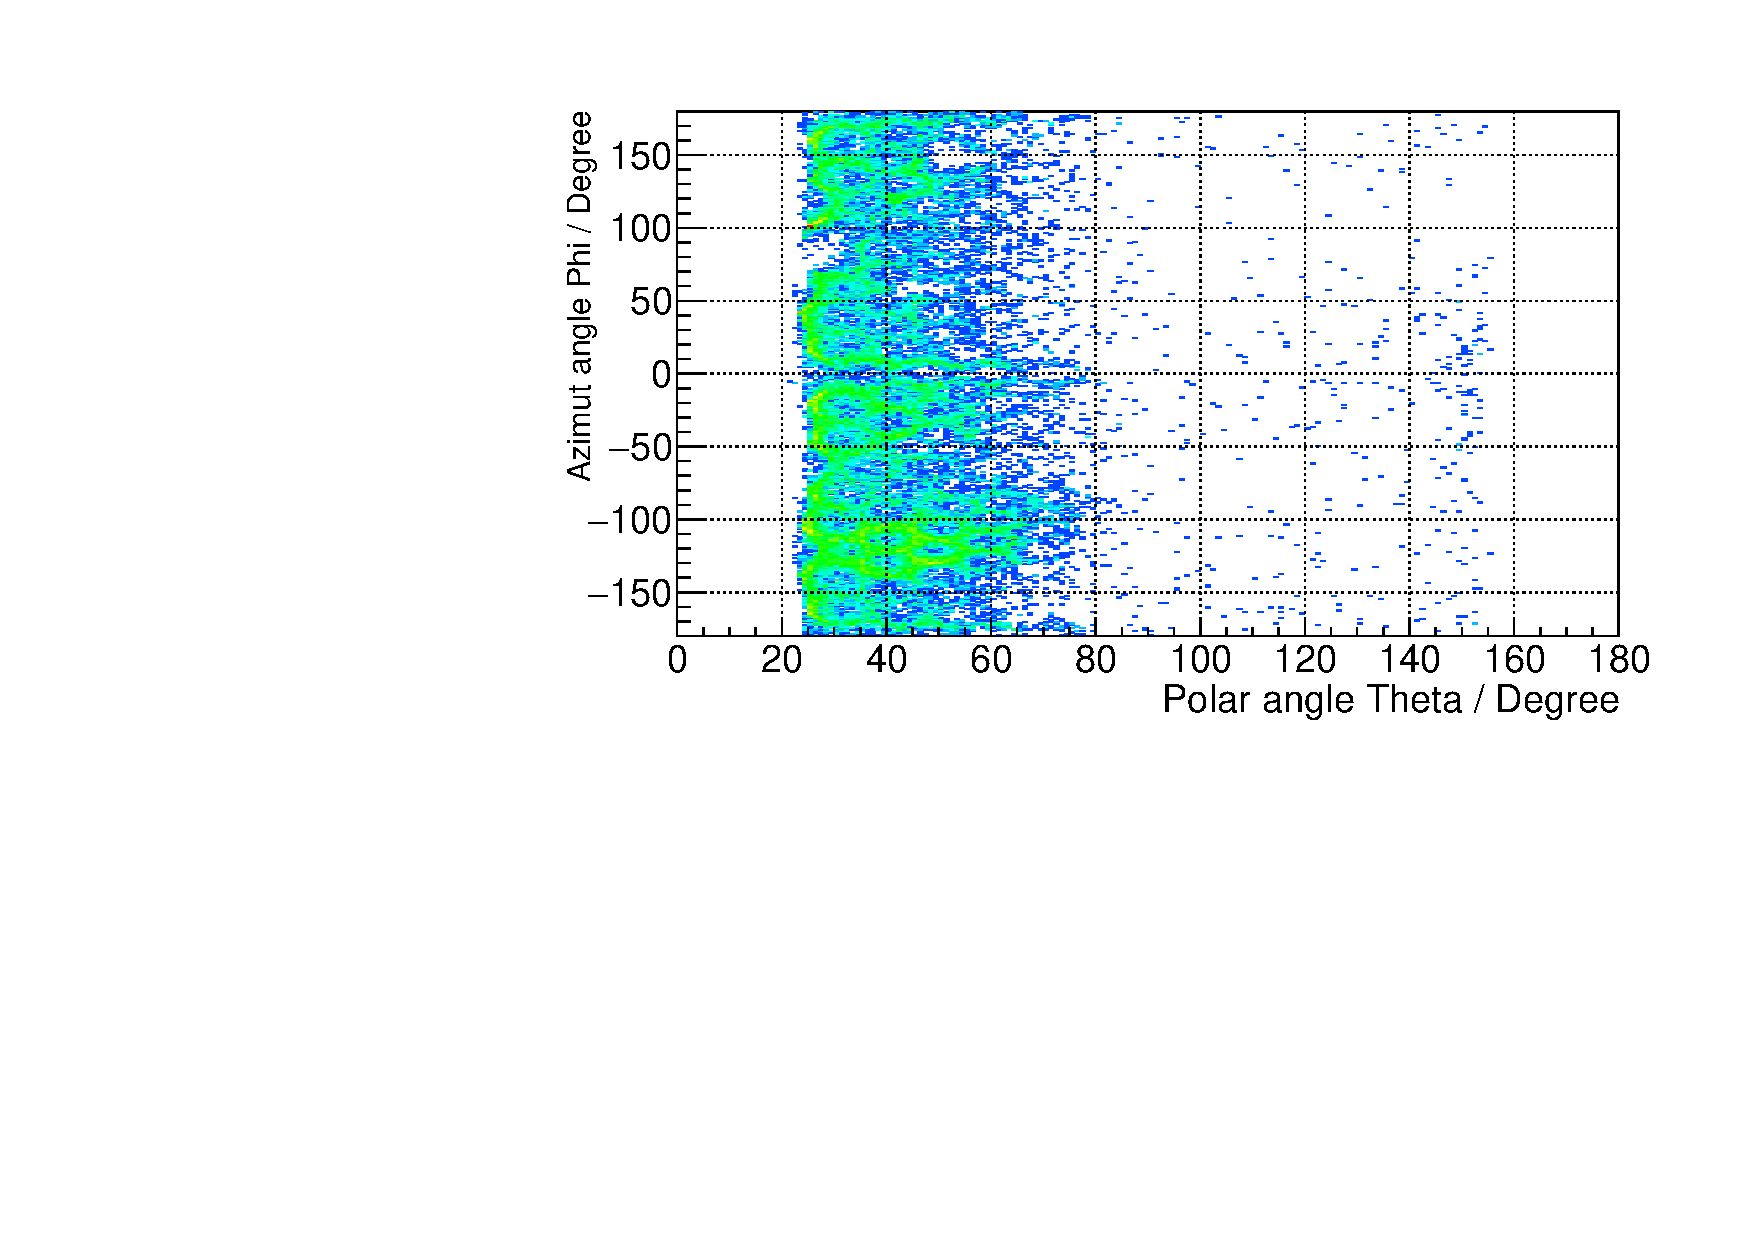
\includegraphics[width=0.9\textwidth]{20170504ThetaPhiEnergySymmetric2014_10_400}
	\end{minipage}
	
	\caption{Links ist die Verteilung der Photonen im Crystal-Ball mit einer Energie von 125 MeV bis 150 MeV zu sehen, rechts von 400 MeV bis 425 MeV. }
\end{figure}

In diesen Abbildungen erkennt man sehr gut, wie sich die Verteilung der Photonen \"andert, wenn die Energie der Photonen zunimmt und die Bedingung gilt, dass sich die Energie der Photonen \"ahneln m\"ussen. So sind die Photonen f\"ur kleine Energien \"uber den ganzen Crystal-Ball verteilt, w\"ahrend f\"ur gr\"o{\ss}ere Energien die Photonen immer h\"aufiger am Strahlenausgang auftreten.

Aus der Verbesserung der Abweichung f\"ur hohe Photonenenergien und unter Vernachl\"assigung der Detektoren am Rand folgte, dass die Detektoren am Rand des Strahleneingangs nicht sehr gut f\"ur hohe Photonenenergien kalibriert sind. Allerdings war damit nicht die gesamte Abweichung zu erkl\"aren, sondern nur bis zu einem Prozent. 
Aussagen \"uber die Detektoren am Strahleneingang konnten ebenfalls nicht getroffen werden, da im Vergleich zum Strahleneingang nur sehr selten getroffen wurde.

Also musste weiter nach der Ursache dieser starken Abweichung gesucht werden.


\section{Simulation}
\label{sec:Z-Vertex-Abaengigkeit}

Da mit reellen Daten keine Ursache gefunden werden konnte, wodurch diese gro{\ss}e Abweichung entstand, wurde auf simulierte Daten zur\"uckgegriffen. 

Der Grund daf\"ur war, dass alle Prozesse in simulierten Daten genau bekannt waren. Das hei{\ss}t von jedem registriertem Teilchen war bekannt, um welches Teilchen es sich gehandelt und aus welchem Prozess es entstanden ist. 

So konnte der ganze Zerfall Schritt f\"ur Schritt auseinander genommen werden, um leichter die Ursache f\"ur die Abweichung zu suchen.

\subsection{Vorbereitung der Simulation}
\label{sec:Vorbereitung-der-Simulation}

Als erstes wurden die Daten aus dem sogenanntem Cocktail entnommen.

Im Cocktail waren ca. 250 Millionen physikalisch m\"ogliche Prozesse enthalten, daher hatte er auch seinen Namen. Folglich waren im Cocktail aber nicht nur $\pi^0 \rightarrow \gamma \gamma$ enthalten, sondern auch alle anderen m\"oglichen. Die Zerf\"alle im Cocktail waren bereits komplett durchsimuliert, wodurch er wie real genommene Daten behandelt werden konnte.

Allerdings stellte sich relativ schnell heraus, dass der Cocktail nicht genug relevante Prozesse enthielt, nachdem alle unerw\"unschten heraus gefiltert wurden. Deshalb wurde zun\"achst ein neues Packet mit mehr Prozessen erstellt.

Dieses Paket beinhaltete Prozesse, welche durch Pluto, eine Monte-Carlo basierende Simulation, generiert wurden. Insgesamt beinhaltete es 10 Millionen $\pi^0 \rightarrow \gamma \gamma$ Prozesse. Das Verhalten des Crystal-Ball Detektors wurde mittels GEANT4\footnote{Geometry And Tracking}, einer Simulation, welche das Durchdringen von Partikeln durch Materie zu beschreibt, simuliert.

Das Erstellen dieses neuen Paketes nahm sehr viel Zeit in Anspruch, da das Simulieren der Detektoren sehr aufw\"andig war. Das Erstellen eines Paketes mit 100000 Prozessen dauerte etwa zwei Stunden. Auch von diesen mussten die meisten verworfen werden, weil Photonen entstanden, deren Energie sich nicht \"ahnelte. So kam es, dass selbst das Paket mit 10 Millionen Prozessen nicht genug Photonenpaare mit \"ahnlicher Energie enthielt.
 
 Um nun aber eine noch größere Simulation zu vermeiden, wurde eine neue $\pi^0$-Gun geschrieben, bei der die gew\"unschten Bedingungen bereits in Pluto f\"ur einen Filter sorgten und so mussten die Teilchen, die sowieso verworfen w\"aren, gar nicht erst durch Geant simuliert werden. 

Da man aber trotzdem keine Informationen \"uber die Prozesse verlieren wollte, mussten alle Schritte des folgendes Zerfalls einzeln untersucht und anschließend in die Gun eingebaut werden.

\begin{equation}
\gamma \rightarrow p + \pi^0 \rightarrow p + \gamma \gamma 
\end{equation}

Da das einfallende Photon durch Bremstrahlung erzeugt wurde, war seine Energie nicht eindeutig, sondern lag in einem gewissen Interval. Also musste als erstes die Energie des Photons gew\"urfelt werden.

Dann begab man sich ins Schwerpunktsystem des einfallenden Photons und des ruhenden Protons $p$. 
Von diesem System konnte dann die Schwerpunktsenergie ausgerechnet werden.

\begin{equation}
\sqrt{s}= \sqrt{2E_{\gamma}m_p+2m_p^2}
\end{equation}

Anschlie{\ss}end wurde angenommen, dass die Reaktion des Protons mit dem Photon ein $\pi^0$ aussendet. Die Richtung in der dieses $\pi^0$ ausgesandt wurde, wurde auch wieder mit einem Zufallsgenerator bestimmt. 

Aufgrund der Impulserhaltung musste gelten, dass der Impuls des Protons in die entgegengesetzte Richtung zum $\pi^0$ zeigte und dass der Betrag der beiden Impulse gleich sein muss. Auch musste aufgrund der Energieerhaltung gelten, dass die Energie der beiden Teilchen gleich der Schwerpunktsenergie war. Es lagen also die folgende Formel vor:

	\begin{equation}
	\sqrt{s}=\sqrt{m_{\pi^0}^2+\overrightarrow{p}^2} + \sqrt{m_{p}^2+\overrightarrow{p}^2}
	\end{equation}

Diese Gleichung konnte nach $|p|$ aufgel\"ost werden. Da die Masse der beiden Teilchen bekannt war, konnte ihr Impuls und damit auch ihre Energie über $E=\sqrt{m^2+p^2}$ ausgerechnet werden. 

Weiter musste angenommen werden, dass das $\pi^0$ instantan in zwei Photonen zerf\"allt. Diese Annahme ist nicht abw\"agig, die Lebenszeit eines $\pi^0$ nur etwa $8,5 * 10^{-17}$ Sekunden betr\"agt. Somit w\"urde es selbst mit Lichtgeschwindigkeit nur ca. 25 nm zur\"ucklegen. Also war die Annahme berechtigt.

Um die Photonen zu erzeugen, begab man sich ins Ruhesystem des $\pi^0$. Die Richtungen, in der die Photonen ausgestrahlt wurden, wurden ebenfalls zuf\"allig bestimmt. Anschlie{\ss}end verlie{\ss} man das Ruhesystem, dazu erhielten die beiden Photonen den Boost des $\pi^0$. 
\newline

In diesem Tool wurde die Energie des Strahls in einem homogenen Interval gew\"urfelt. Dies entspricht nicht der Realit\"at, da die Energieverteilung von Photonen, welche durch Bremsstrahlung erzeugt werden, nicht gleichm\"a{\ss}ig ist, sondern im gew\"unschtem Interval eher an eine $1/x$-Verteilung erinnert. Folglich wurden in meinem Tool deutlich mehr hochenergetische Bremsstrahlphotonen erzeugt. Dies war allerdings nur nebensächlich, da ich in meinen Untersuchungen nur sicherstellen musste, das alle im Experiment auftretenden Photonen auch in meiner Simulation auftreten.

Es musste also noch überprüft werden, ob die Form der Verteilung der neuen $\pi^0$-Gun, der alten entsprach. Dazu wurde die alte Gun ebenfalls so eingestellt, dass die Energieverteilung des eintreffenden Photonenstrahls homogen verteilt war, dadurch war ein einfacherer Vergleich möglich. 


\begin{figure}[h!]
	\centering
	\begin{minipage}{0.45\textwidth}
		\centering
		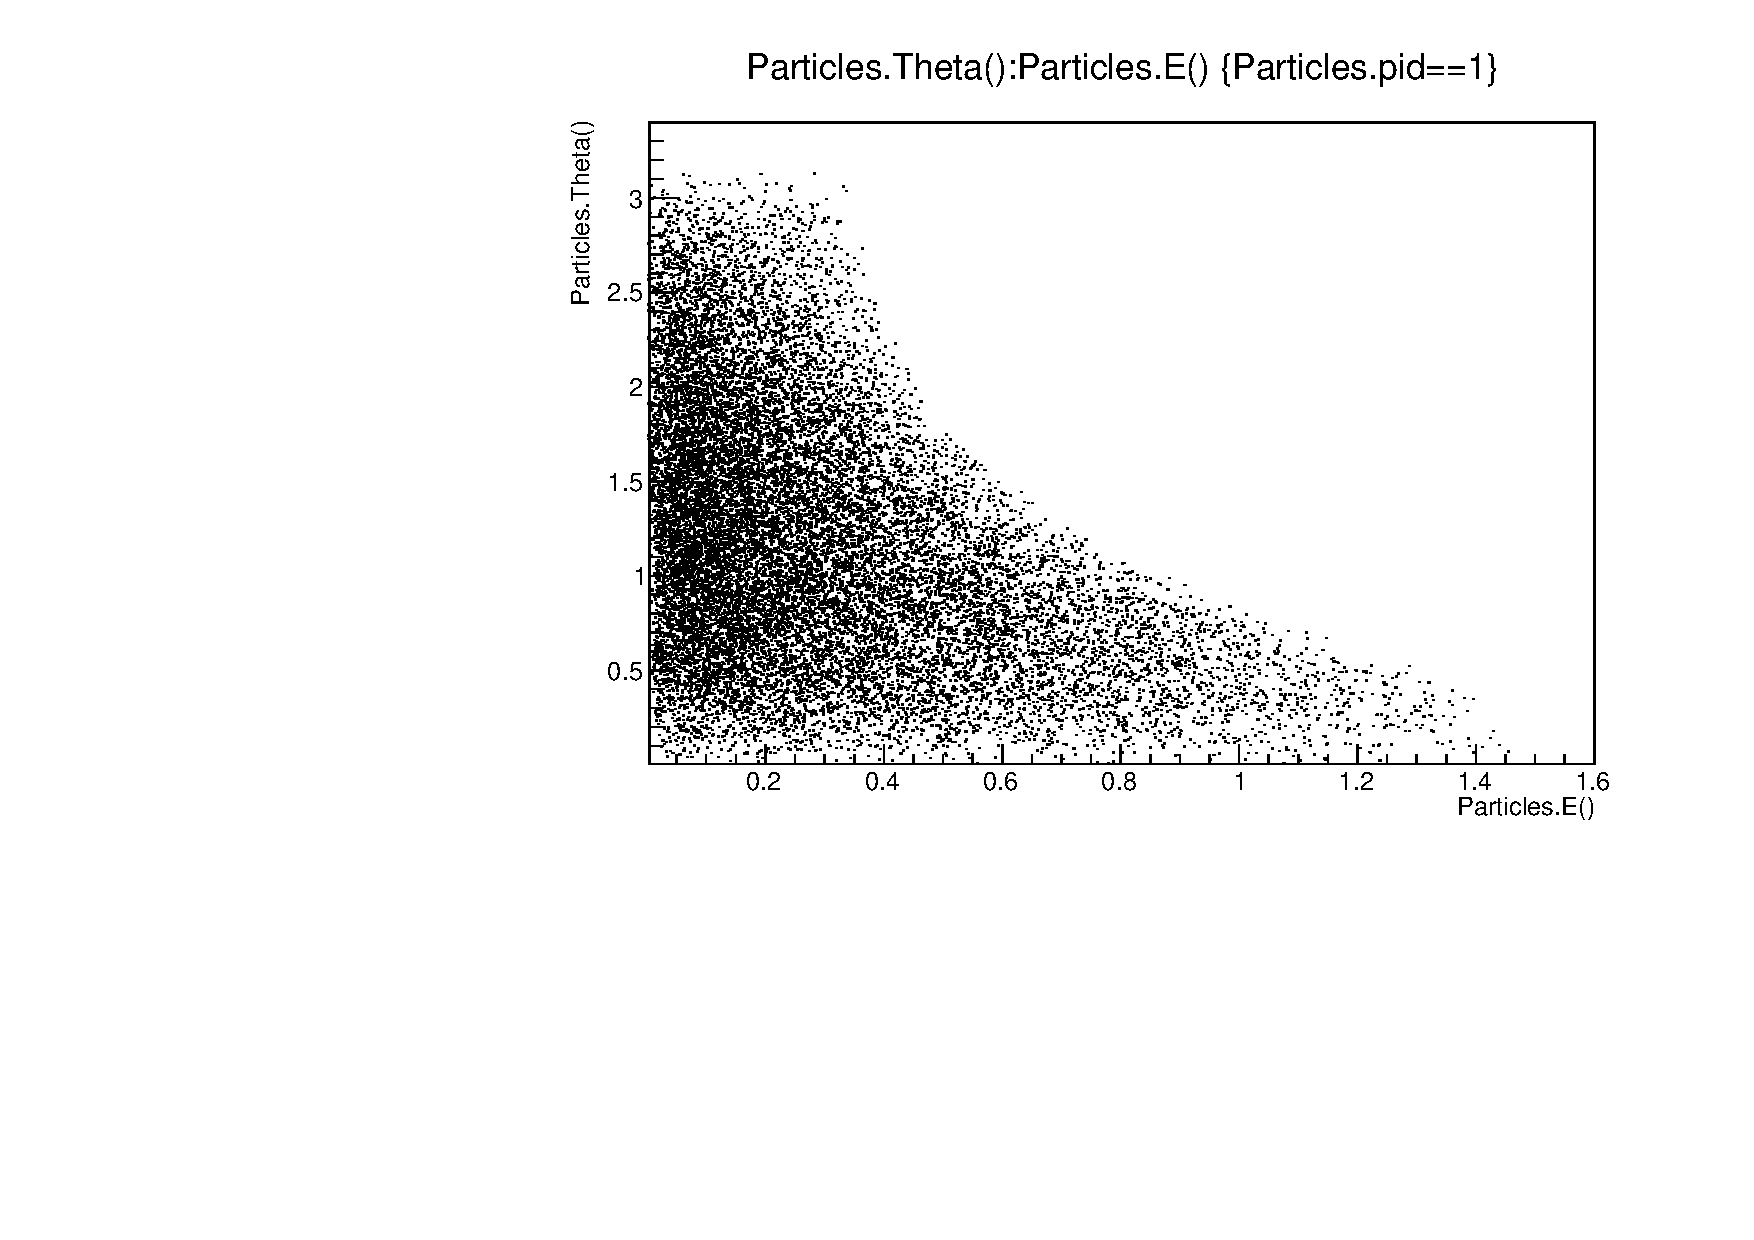
\includegraphics[width=0.9\textwidth]{20170704Pi0_Gun_New}
	\end{minipage}
	\hfill
	\begin{minipage}{0.45\textwidth}
		\centering
		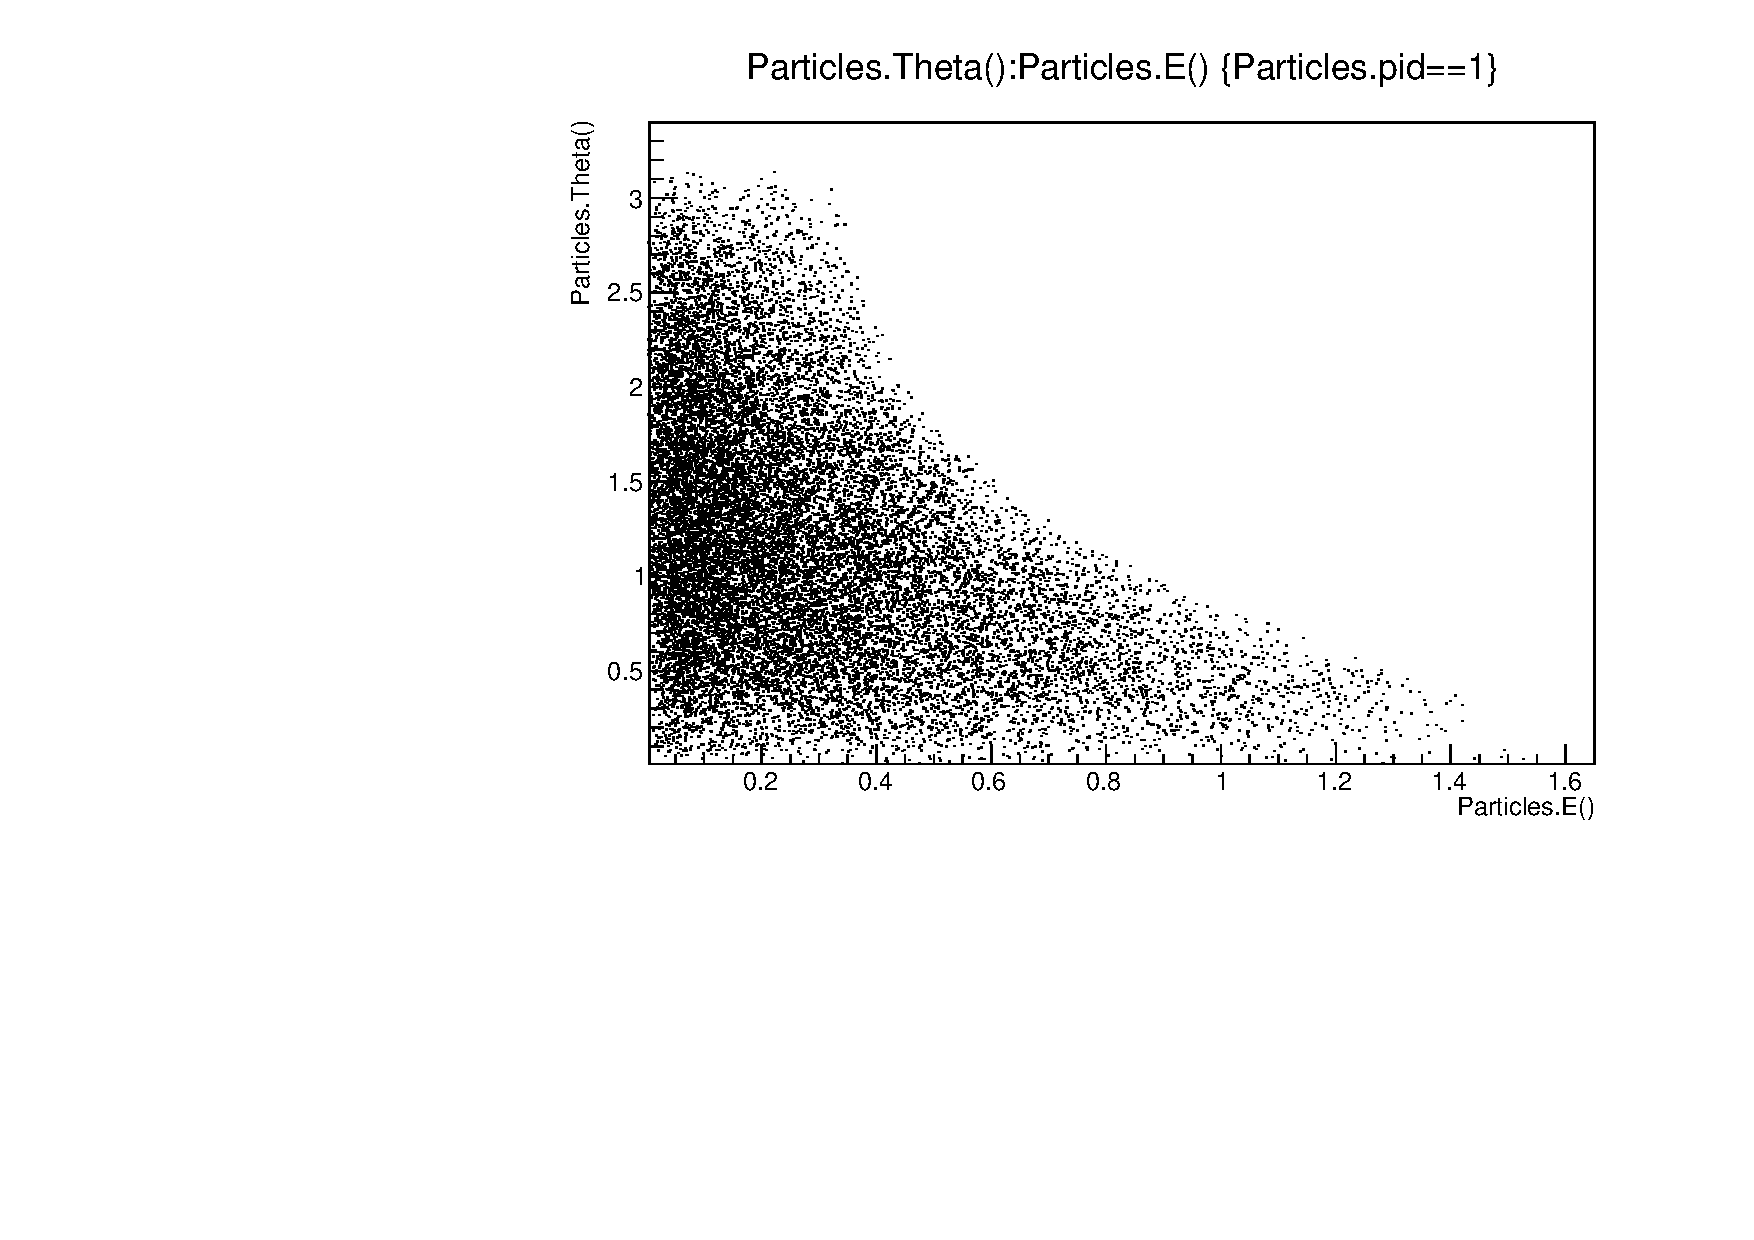
\includegraphics[width=0.9\textwidth]{20170704Pi0_Gun_Old}
	\end{minipage}
	
	\caption{Links wurde die neue und rechts die alte Gun benutzt. Aufgetragen wurde der Winkel in Radiant gegen die Energie in GeV der durch den Zerfall ausgesandten Photonen. Auch bei diesen Plots erkennt man, dass höherenergetische Photonen eher am Strahlenausgang vorliegen.}
	\label{fig:Vergleich-der-beiden-Guns}
\end{figure}

In diesen beiden Abbildungen erkennt man, dass sich die Form der Verteilung stark ähneln. Also konnte angenommen werden, dass die neue $\pi^0$-Gun wie gewünscht funktionierte.
\newline

Als nächstes musste noch \"uberpr\"uft werden, ob die in Kapitel \ref{sec:Energie-Interval-Abhaengigkeit} und \ref{sec:Vernachlaessigung-der-Detektoren-am-Rand} gefundene Abh\"angigkeit auch in der Simulation auftrat. 
Dazu wurden zwei Histogramme mit den Bedingungen aus den jeweiligen Kapiteln gef\"ullt. Eins mit den Detektoren am Rand und eins ohne.

\colorbox{yellow}{Die beiden Histogramme aus den Simulierten Daten}

An den beiden Histogrammen erkennt man, dass es sich bei den verwendeten Daten um Simulierte gehandelt hat, da der $\eta$-Peak nicht vorhanden ist. Man hat nur noch einen Peak bei $\pi^0$. 

 \"Uber diese wurde dann auch wieder mit der Crystal-Ball-Funktion gefittet, um die $\pi^0$ Position zu bestimmen.

Auch hier wurden die beiden Abweichungen zum besseren Vergleich in einen einzelnen Graphen gezeichnet.

%Da bei einer Simulation alle Prozesse genau bekannt waren, wurde alles so eingestellt, dass aus dem Cocktail nur $\pi^0 \rightarrow \gamma \gamma\ $ Prozesse betrachtet wurden.

\colorbox{yellow}{Hist von Simulierten Daten + Abweichung Simulierte Daten ohne Dek. am Rand}


Auch hier ist die Abweichung zu erkennen. Folglich k\"onnen nun weitere Aspekte mit der Simulation \"uberpr\"uft werden.
%Ein weiterer Vorteil einer Simulation war, dass man von jedem detektierem Teilchen wusste, woher es kam und worum es sich dabei handelte. Folglich konnte alles so eingestellt werden, dass aus dem Cocktail nur $\pi^0 \rightarrow \gamma \gamma$ Prozesse betrachtet wurden.

\subsection{Zerfall von $\pi^0$ im Ursprung}

Als erstes wurde \"uberpr\"uft, wie sich die Detektoren verhielten, wenn das $\pi^0$ im Ursprung zerf\"allt, dabei durfte das Pion einen Boost in eine beliebige Raumrichtung haben, wodurch es keine ausgezeichneten Detektoren mehr gab. Somit konnte ein Vergleich gezogen werden, ob sich alle Detektoren gleich verhielten. 

Dazu wurde die neue $\pi^0$-Gun so eingestellt, dass es keinen Photonenstrahl und kein Proton mehr gab, lediglich der Boost des $\pi^0$ wurde gewürfelt. Die Photonen wurden dann anschließend wie in \ref{sec:Vorbereitung-der-Simulation} beschrieben gewürfelt und geboostet. 
Als erstes wurde \"uberpr\"uft, ob die durch den Zerfall ausgesandten Photonen sich auch wirklich gleichm\"a{\ss}ig im Raum verteilten.
\begin{figure}[h!]
	\begin{center}
		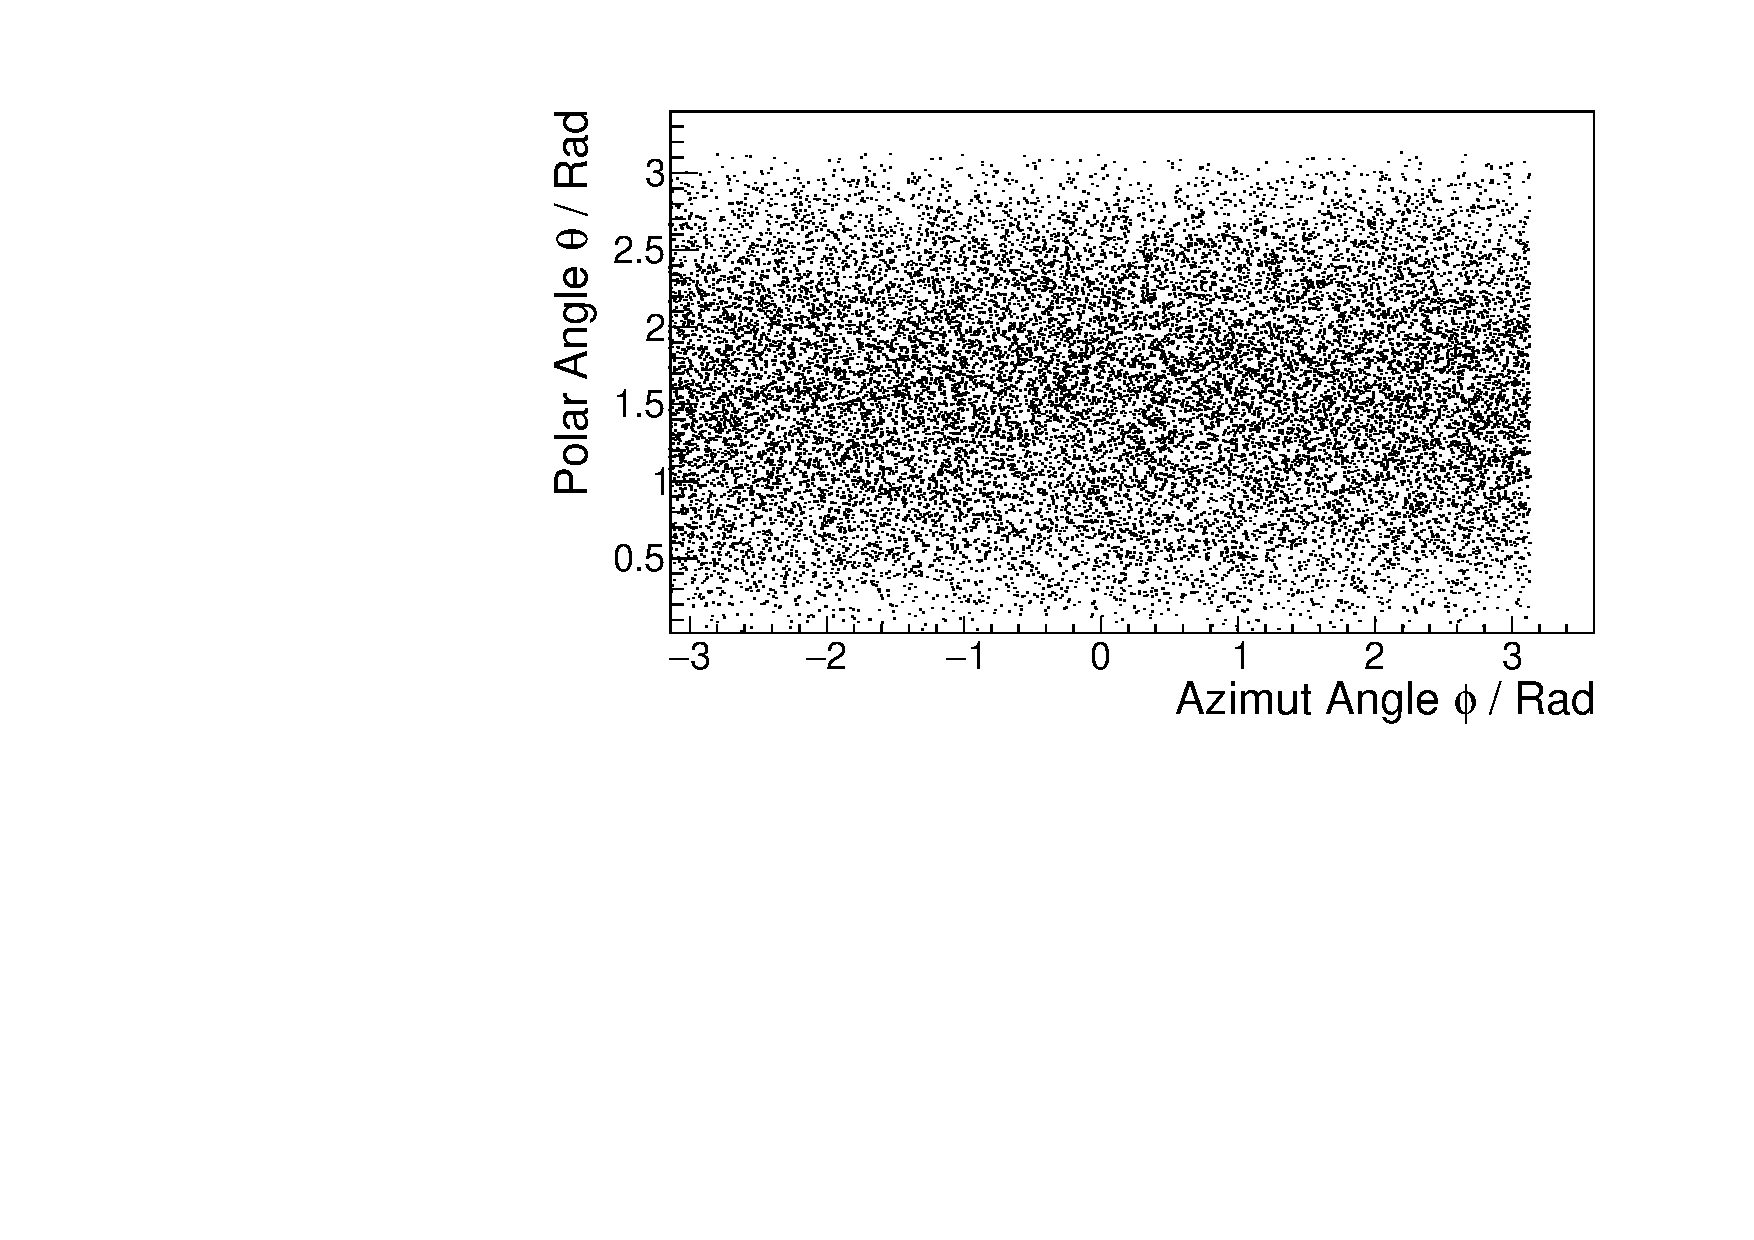
\includegraphics[width=100mm]{20171005Pi0UrsprungThetaPhiVerteilung}
		\caption{Verteilung der ausgesandten Photonen im Raum.}
	\end{center}
\end{figure}

In dieser Abbildung erkennt man, dass sich die Photonen isotrop verteilt haben. Folglich f\"uhrte das Tool den Boost des $\pi^0$ in eine zuf\"allige Richtung richtig aus.

Zus\"atzlich galt die Bedingung, dass nur Photonen mit einer ähnlichen Energie als Ereignis in die Datei geschrieben werden durften.

In GEANT wurde die Länge des Target auf 0 cm gesetzt. Dadurch wurde gewährleistet, dass die Pionen auch wirklich im Ursprung zerfallen.


%Au{\ss}erdem ben\"otigte das Simulieren des Crystal-Balls sehr viel Zeit. So dauerte es zum Simulieren von 100000 Prozessen etwa zwei Stunden. Von diesen mussten die meisten verworfen werden, weil Photonen entstanden, deren Energie sich nicht \"ahnelte. Folglich w\"urde man ein Packet mit mehreren Millionen reinen $\pi^0 \rightarrow \gamma \gamma $ Prozessen ben\"otigen, um genug Ereignisse zu erhalten. So wurde ein Paket benutzt, welches 10 Millionen dieser Prozesse beinhaltete, allerdings war es trotzdem nicht gro{\ss} genug, um eine gute Statistik zu erhalten. gr\"o{\ss}ere Pakete existierten nicht.

%Um nun  eine lange Simulaiton zu vermeiden, wurde beim Erstellen der Simulation \"uber Pluto, bereits hier die Energie der beiden Photonen \"uberpr\"uft. Nur dann wurde der Zerfall von Pluto eingetragen und anschlie{\ss}end \"uber GEANT4 simuliert. Dies hatte eine erhebliche Zeitersparnis zur Folge.

Um zu überprüfen, ob alles wie gewollt eingestellt war, reichte es die Winkel der Pionen gegen ihre Energie aufzutragen. 

Hier ist zu erkennen, dass sich die Pionen gleichm\"a{\ss}ig im Raum verteilen und es keine ausgezeichnete Richtung gab. Also wurde alles wie gew\"unscht eingestellt, wodurch das weitere Verhalten des Crystal-Balls betrachtet werden konnte.

Nun wurde \"uberpr\"uft, wie sich die Abweichung des $\pi^0$-Peaks verhielt, wenn das $\pi^0$ einen zuf\"alligen Boost in eine beliebige Richtung erhielt. Dazu wurde ein dreidimensionales Histogramm angelegt, mit der errechneten invarianten Masse auf der x-Achse, der Energie der Photonen auf der y-Achse und der Energie des geboosteten Mesons auf der z-Achse. Es galt immer noch die Bedingung, dass die detektierten Photonen eine \"ahnliche Energie aufweisen mussten, um in das Histogramm gef\"ullt zu werden.

\colorbox{yellow}{Weitere Auswertung fehlt noch}


\subsection{Z-Vertex Abh\"angigkeit}

Auch wurde die Abh\"angigkeit, zwischen der errechneten  Position des $\pi^0$-Peaks und dem Ort im Target in dem das Pion entstanden und zerfallen war, \"uberpr\"uft. 

In Kapitel \ref{sec:Vorbereitung-der-Simulation} wurde gezeigt, dass das $\pi^0$ maximal 25 nm zurücklegen kann. Folglich konnte angenommen werden, dass das Pion am gleichem Ort zerf\"allt, an dem es auch entsteht.

% Hier wurde schlie{\ss}lich ein weiterer Vorteil der Simulation ausgenutzt. Bei einer Simulation sind alle Prozesse genau bekannt. Von jedem Prozess wusste man demnach auch den genauen Ort an dem er sich ereignete. Bei reellen Messdaten war dies nicht m\"oglich, da der Crystal-Ball keinen Detektor besa{\ss}, um den Ort des Zerfalls zu bestimmen. 
 
Zur Untersuchung der Z-Vertex Abhängigkeit wurde das 10 cm lange Fl\"ussig-Wasserstoff-Target im Zentrum des Crystal-Ball Detektor in zehn 1 cm lange Intervalle unterteilt. 
Im Zentrum des Targets befand sich der Ursprung des Koordinatensystems, so lag am Anfang des Targets das Intervall von z=-5 cm bis z=-4 cm, dann folgte z=-4 cm bis z=-3 cm usw. 

Hier wurde ein weiterer Vorteil der Simulation ausgenutzt. Aus den im Experiment genommenen Daten konnte n\"amlich nicht der Ort bestimmt werden, an dem das $\pi^0$ zerfallen war. Daf\"ur gab es keine Detektoren im Crystal-Ball. In Simulationen waren alle Prozesse allerdings wohl bekannt. So wusste man auch von jeden Prozess an welchem Ort er sich ereignete. 

 Anschließend wurde ein dreidimensionales Histogramm angelegt mit den Intervallen des Z-Vertex auf der z-Achse, der errechneten invarianten Masse auf der x-Achse und der Energie der Photonen auf der y-Achse angelegt. 

Daraus konnte dann die Position des $\pi^0$-Peaks in Abhängigkeit zum Z-Vertex Intervall berechnet werden, dazu wurde jedes Z-Intervall einzeln betrachtet und die Position abhängig von der Energie der Photonen berechnet.
Diese 10 Z-Vertex Abhängigkeiten wurden anschließend in Abbildung \ref{fig:Z-Vertex-Multi-Graph} eingetragen.

\begin{figure}[h!]
	\begin{center}
		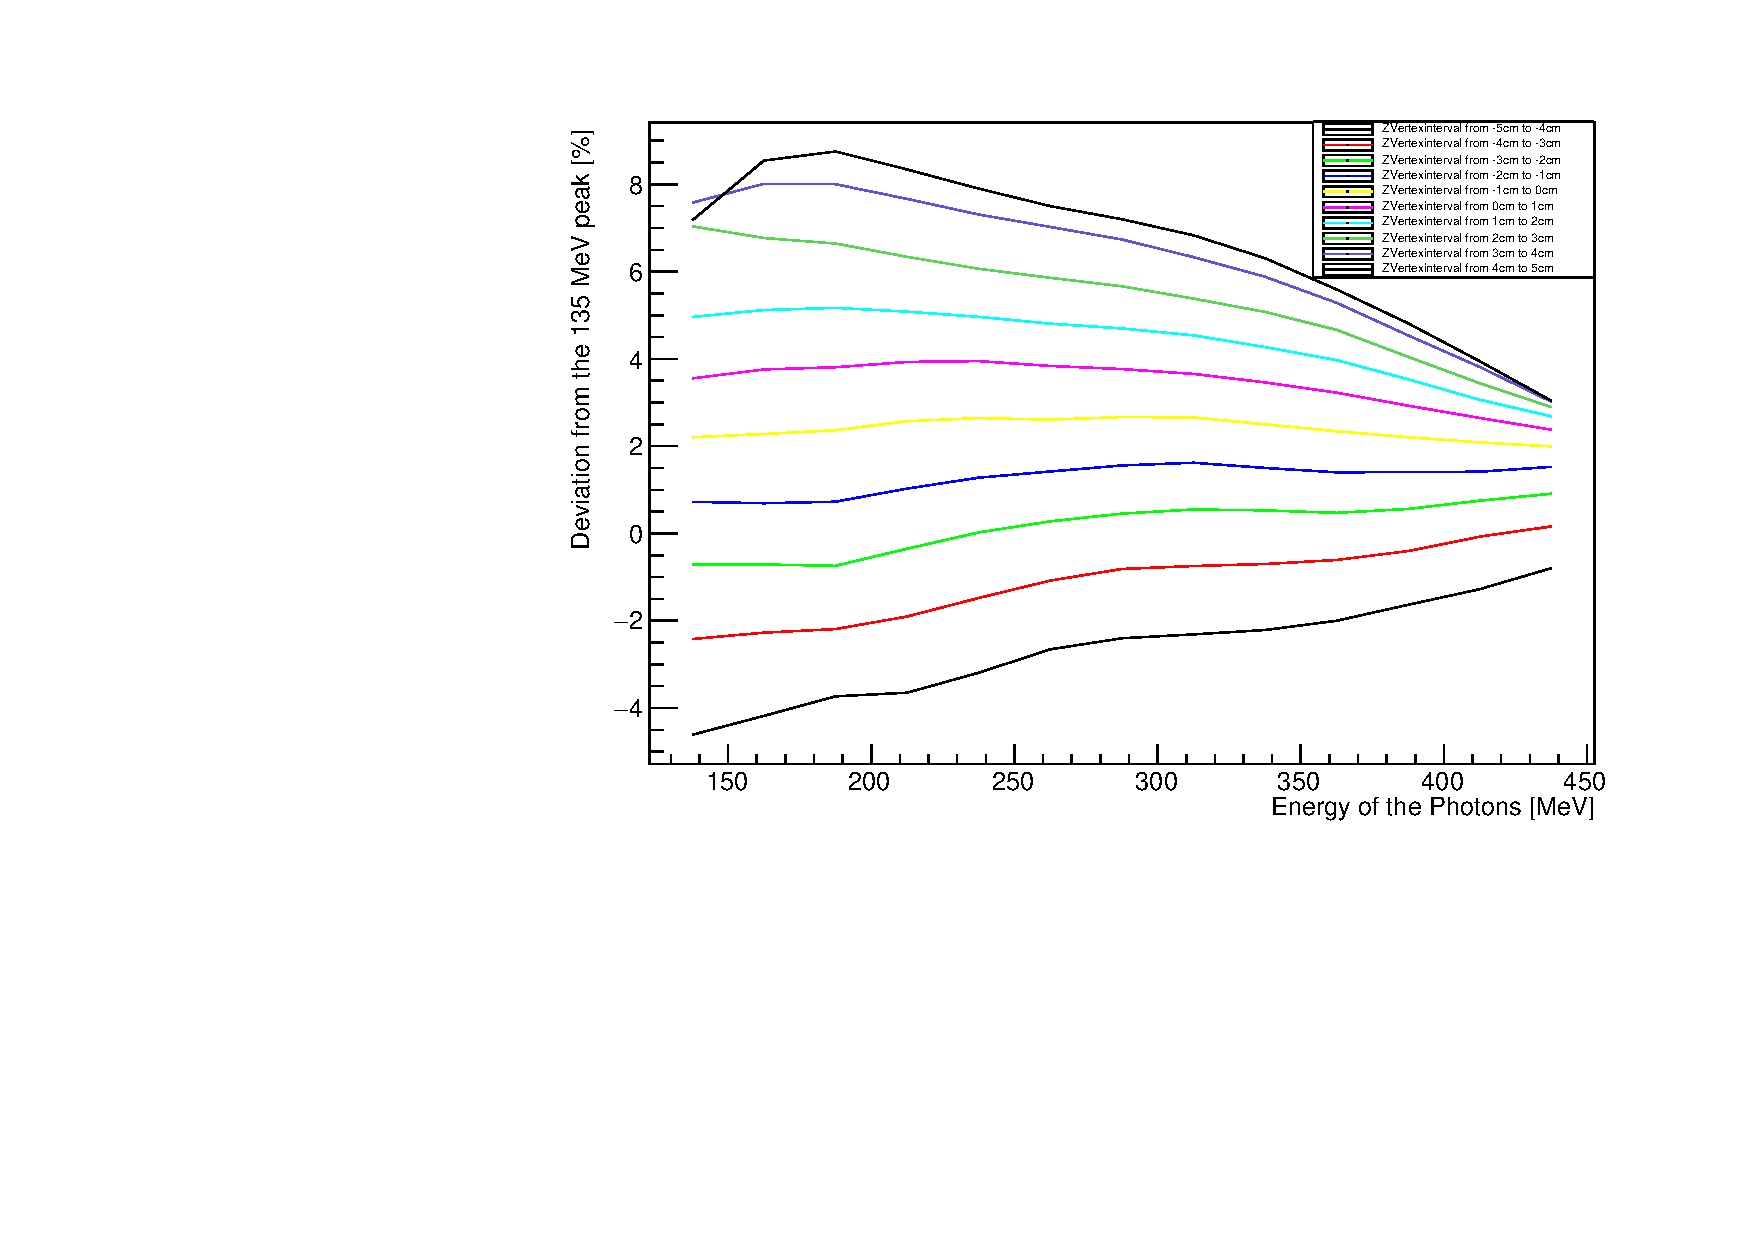
\includegraphics[width=100mm]{FullZVertexDependence}
		\caption{Die Abweichung der $\pi^0$-Peak Position für verschiedene Intervalle des Z-Vertex gegen die Energie der gemessenen Photonen. Beachte: Die unterste Linie repr\"asentiert das Intervall von -5 cm bis -4 cm, das dar\"uber von -4 cm bis -3 cm usw.}
		\label{fig:Z-Vertex-Multi-Graph}
	\end{center}
\end{figure}

Wie zu erwarten war, ergaben verschiedene Z-Vertices unterschiedliche Abweichungen des Peaks. So war die Abweichung gr\"o{\ss}er, wenn die Bedingung galt, dass das $\pi^0$ am Rand des Targets zerf\"allt, als wenn nur Zerf\"alle in der Mitte des Targets betrachtet wurden. Dies lag daran, das zur Kalibrierung des Crystal-Ball angenommen wurde, dass das Meson im Zentrum des Targets zerf\"allt. Das hatte zur Folge, dass der Winkel aus Gleichung \ref{eq:Formel-zur-Berechnung-der-invarianten-Masse} verf\"alscht wurde, wenn ein Zerfall au{\ss}erhalb des Zentrum des Targets betrachtet wurde. Der Grund daf\"ur war, dass beim Zerfall des $\pi^0$ die meisten hochenergetischen Photonen in Strahlrichtung entstehen\footnote{Siehe dazu Kapitel \ref{sec:Vernachlaessigung-der-Detektoren-am-Rand} Ende}. Folglich hoben sich die Abweichungen im Winkel nicht mit der Statistik weg, sondern es gab eine inhomogene Verteilung der Winkel. 
  
Auch zu sehen ist, dass der Abstand der Linien f\"ur niedrige Energie, fast durchgehend, ca. 1\% betrug, ausgenommen ist das Intervall von -5 cm bis -4 cm. Ebenfalls war zu erkennen, dass die einzelnen Abweichungen sich f\"ur gr\"o{\ss}ere Energien der ca. 2\% Abweichung ann\"aherten. Eine solche Abweichung war bereits in Kapitel \ref{sec:Reelle-Daten} zu erkennen, dort wurde der Z-Vertex nicht in Intervalle unterteilt, sondern als ganzes betrachtet.

Da auch in den simulierten Daten diese Abweichung der $\pi^0$-Peak Position zu erkennen war, musste genauer nach der Ursache gesucht werden.


%_______________________________________________________________________________
\chapter{Zusammenfassung und Ausblick}

%In der Zusammenfassung sollten Sie in knapper Form die Aufgabenstellung 
%und die wichtigsten Ergebnisse rekapitulieren. Es ist f\"ur die 
%Gutachter hilfreich, wenn Sie ausdr\"ucklich beschreiben, worin 
%Ihre eigenen Beitr\"age liegen. Scheuen Sie sich auch nicht davor 
%auszusprechen, welche Untersuchungen durch die Zeitbegrenzung der 
%Bachelorarbeit nicht m\"oglich waren und nutzen Sie dies als 
%\"Uberleitung zu einem Ausblick auf m\"ogliche weitergehende 
%Arbeiten an der Aufgabenstellung.

%_______________________________________________________________________________
\begin{appendix}
\chapter{Anhang}
\section{Herleitung der Formel zur Berechnung der invarianten Masse}
\label{sec:Herleitung-der-Formel-zur-Berechnung-der-invarianten-Masse}

Man betrachte die drei Viererimpulse f\"ur den Prozess: $\pi^0\rightarrow \gamma\gamma $
\begin{equation}
p_{\pi^0}^{\mu}=\left(\begin{array}{c}E_{\pi^0}\\\overrightarrow{p_{\pi^0}}\end{array}\right) \textnormal{,  }
p_{1}^{\mu}=\left(\begin{array}{c}E_{1}\\\overrightarrow{p_{1}}\end{array}\right) \textnormal{ und  } p_{2}^{\mu}=\left(\begin{array}{c}E_{2}\\\overrightarrow{p_{2}}\end{array}\right)
\end{equation}

Dabei sind $E_{1}$ und $E_{2}$ die Energien und $\overrightarrow{p_{1}}$ und $\overrightarrow{p_{2}}$ die Impulse der beiden Photonen und $E_{\pi^0}$ die Energie und $\overrightarrow{p_{\pi^0}}$ der Impuls des Pion.

Aufgrund der Energie- und Impulserhaltung gilt:
\begin{equation}
p^{\mu}_{\pi^0} = p^{\mu}_1 + p^{\mu}_2
\end{equation}

Diese Gleichung kann nun quadriert werden:

\begin{equation}
\begin{split}
\rightarrow \underbrace{p^{\mu^2}_{\pi^0}}_{m_{\pi^0}^2}=& (p_{1}^{\mu}+p_{2}^{\mu})^2 \\ 
\rightarrow m_{\pi^0}^2=& \underbrace{p_{1}^{\mu^2}}_{=m_1^2}+\underbrace{p_{2}^{\mu^2}}_{=m_2^2}-2p_{1}^{\mu}p_{2}^{\mu} \\ 
=& m_1^2+m_2^2-2E_1E_2+2\overrightarrow{p_1}\overrightarrow{p_2} \\ 
=& m_1^2+m_2^2-2E_1E_2+2|\overrightarrow{p_1}| |\overrightarrow{p_2}| cos(\vartheta) \\
&\textnormal{mit } \vartheta=\sphericalangle(\overrightarrow{p_1},\overrightarrow{p_2})
\end{split}
\end{equation}

Da man sich nur f\"ur die Photonen interessierte, konnte angenommen werden, dass es sich bei den Teilchen um Photonen handelt. Daraus folgt das $|\overrightarrow{p_1}|=E_1$ und $|\overrightarrow{p_2}|=E_2$ und $m_1=m_2=0$ gilt.

Damit lässt sich die invariante Masse des Pions, welches in die beiden Photonen zerfallen ist, durch
\begin{equation}
\begin{split}
\Rightarrow{m_{\pi^0}=\sqrt{2E_1E_2(1-cos(\vartheta))}}
\label{eq:Formel-zur-Berechnung-der-Invariante-Masse-Herleitung}
\end{split}
\end{equation}
berechnen.

Durch den Crystal-Ball waren alle Variablen in dieser Gleichung bekannt. So konnte die Energie der Photonen bestimmt werden und durch Kenntnis des Auftreffortes der Photonen im Crystal-Ball konnte der Winkel zwischen den beiden Photonen errechnet werden, dazu musste allerdings angenommen werden, dass das $\pi^0$ im Zentrum des Targets zerfällt. Siehe dazu Kapitel \ref{sec:Z-Vertex-Abaengigkeit}.

\section{Tabellen und Abbildungen}

%In der Regel sind die in Tabellen und Abbildungen enthalten Informationen 
%so wichtig, dass sie im Hauptteil der Arbeit erscheinen sollten. Unter 
%Umst\"anden sind aber erg\"anzende Tabellen und Abbildungen gut in einem 
%Anhang aufgehoben. Wie im Hauptteil sollten Sie auch hier darauf achten, 
%dass die in Tabellen und Figuren (siehe Abb.\ \ref{Abb:1}) dargestellte 
%Information im Text angesprochen wird und selbsterkl\"arende Legenden 
%vorhanden sind.
%\medskip

\begin{figure}[h!]
	\begin{center}
		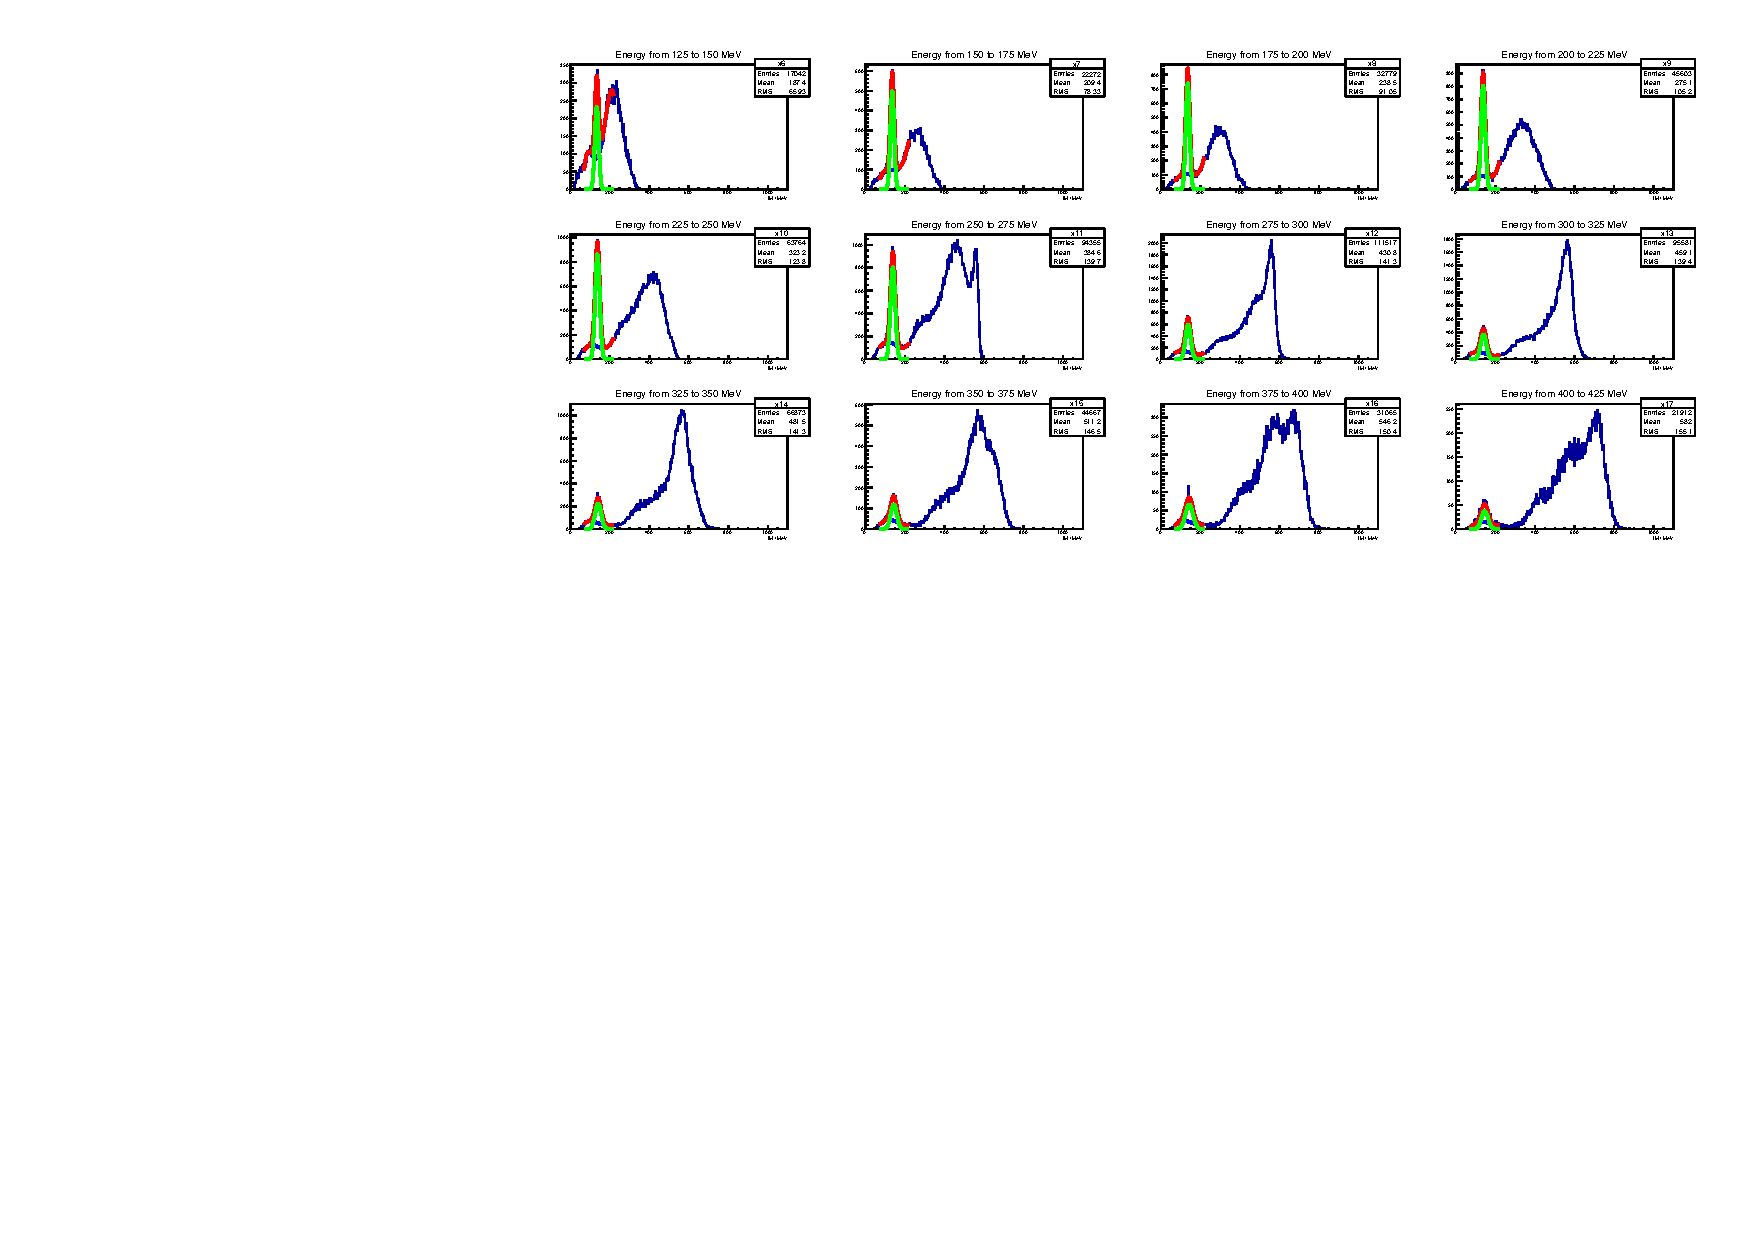
\includegraphics[width=100mm]{RealDataEnergyIntervalSymmetricPhotonsAllFits}
		\caption{Alle Fits der Energieintervalle mit der Bedingung, dass sich die Photonen sich energetisch ähneln.}
		\label{fig:similarenergyallfits}
	\end{center}
\end{figure}

\begin{figure}[h!]
	\begin{center}
		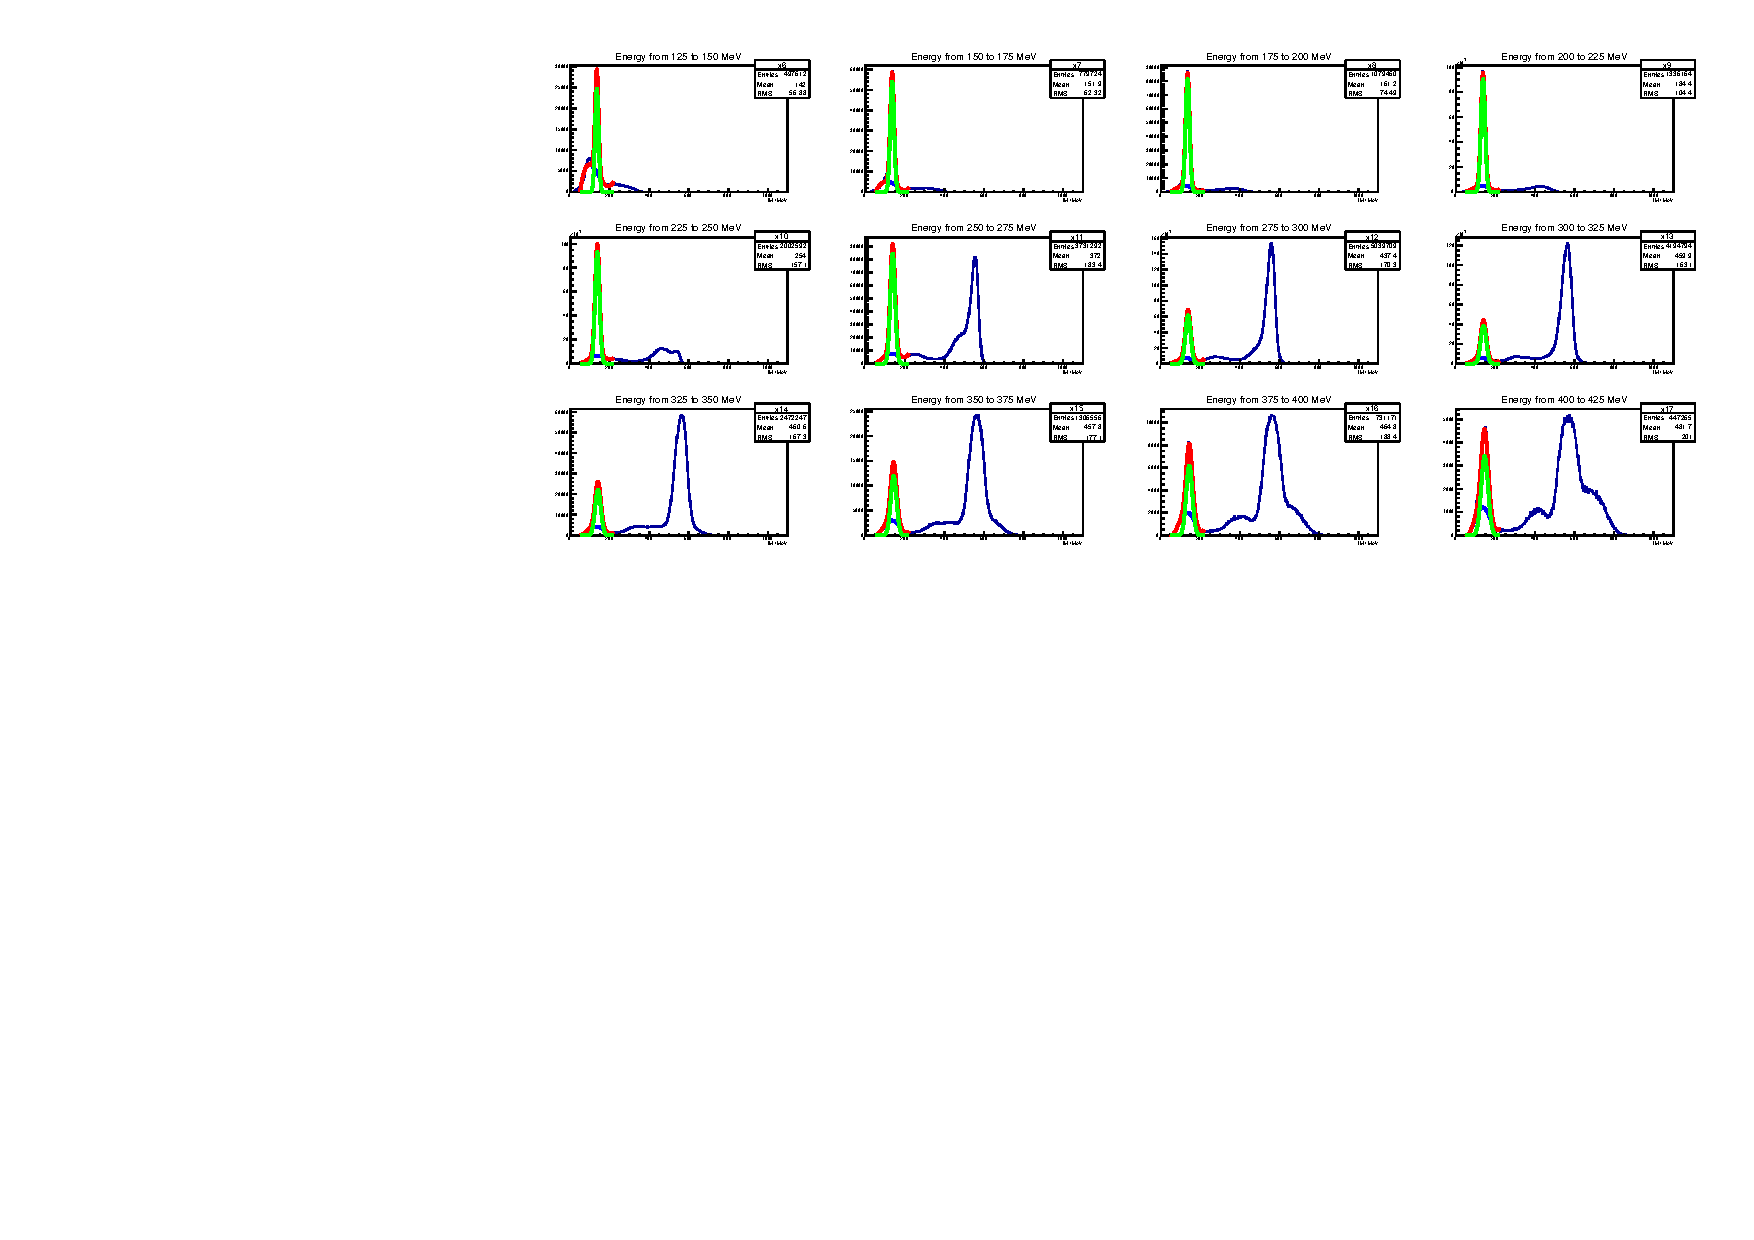
\includegraphics[width=100mm]{EnergyIntervalAllFitsUncharged}
		\caption{Alle Fits der Energieintervalle mit der Bedingung, dass sich die Photonen sich energetisch ähneln und dass die detektierten Teilchen ungeladen sind.}
		\label{fig:similarenergyallfitsuncharged}
	\end{center}
\end{figure}

\begin{figure}[h!]
	\begin{center}
		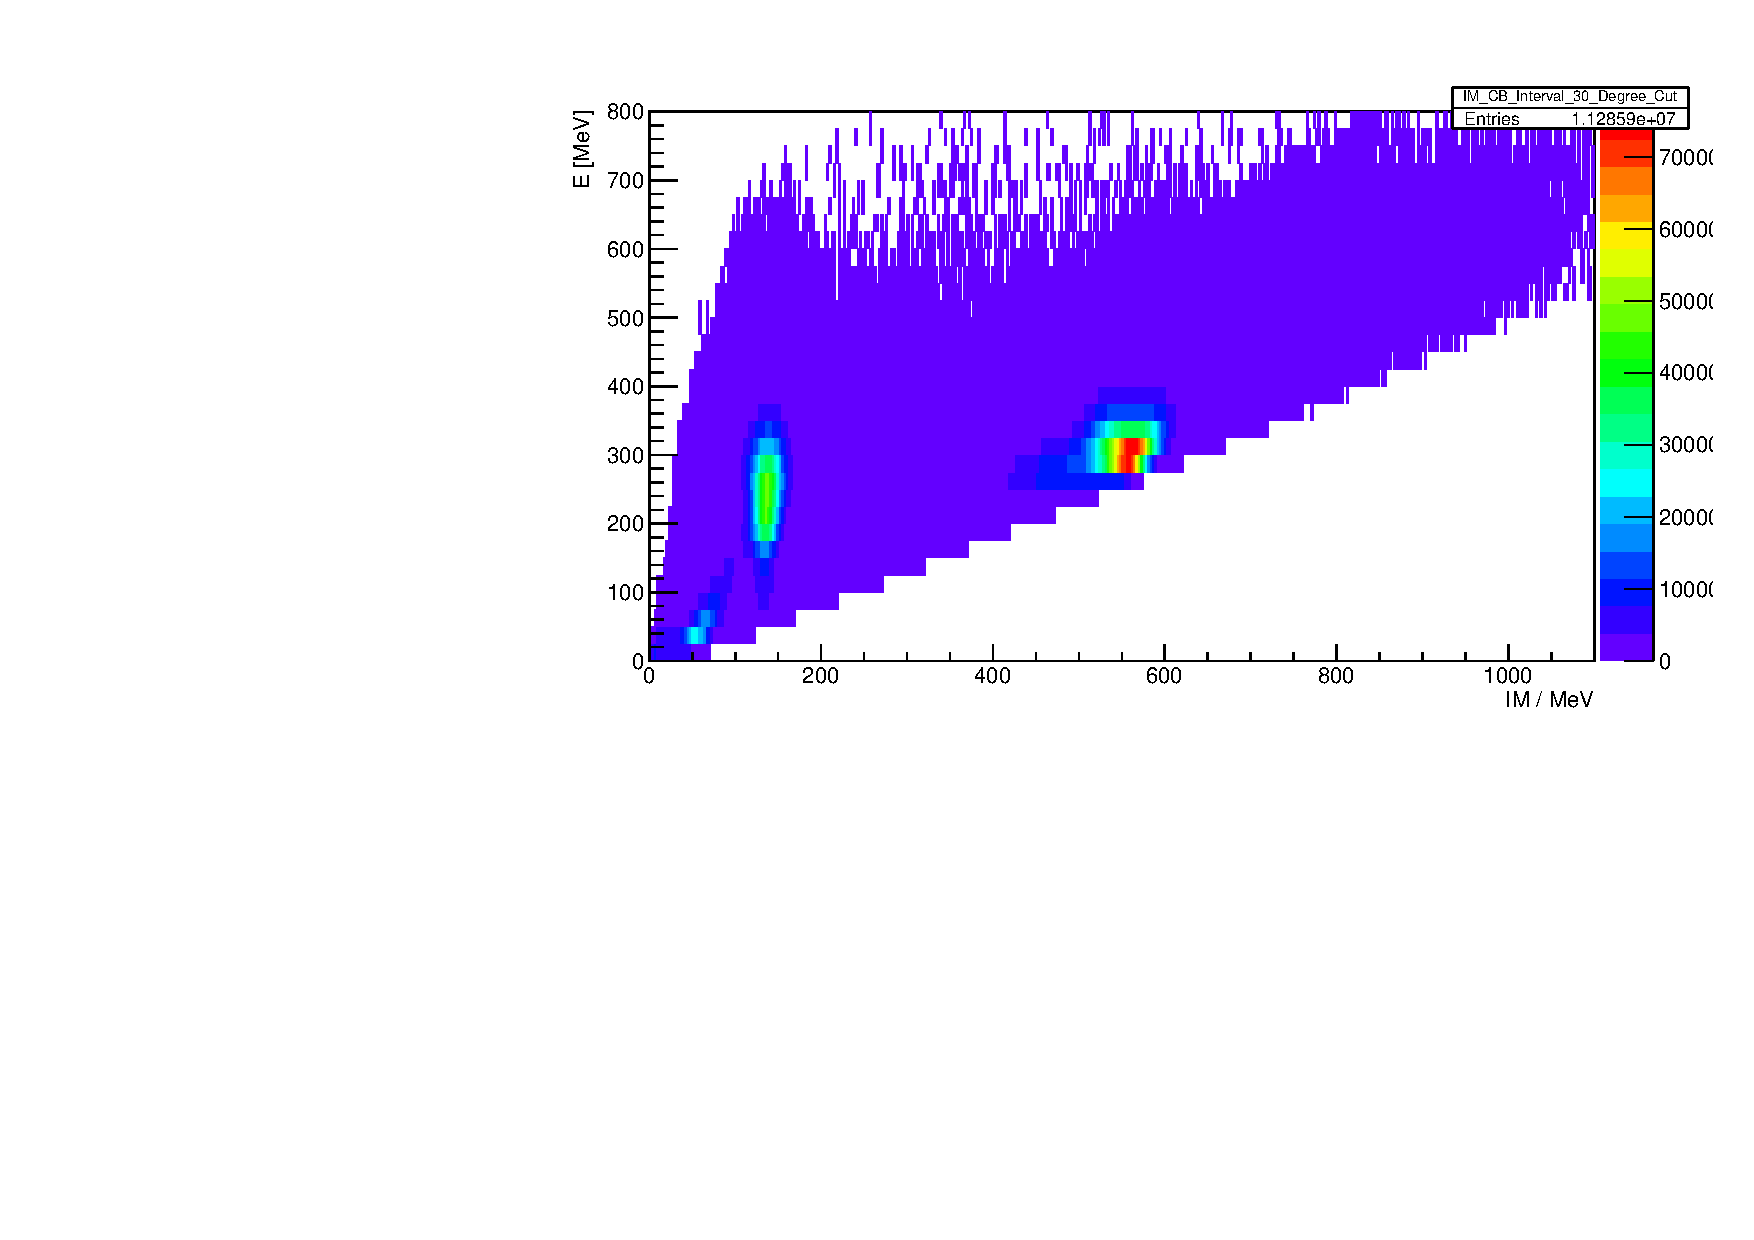
\includegraphics[width=100mm]{30DegreeCutHistRealData}
		\caption{Das Histogramm das gef\"ullt wurde mit der Bedingung, dass sich die Energie der Photonen \"ahneln muss und dass die Detektoren am Rand vernachl\"assigt wurden.}
		\label{fig:30-Degree-Cut-Histogramm}
	\end{center}
\end{figure}


\begin{figure}[h!]
	\begin{center}
		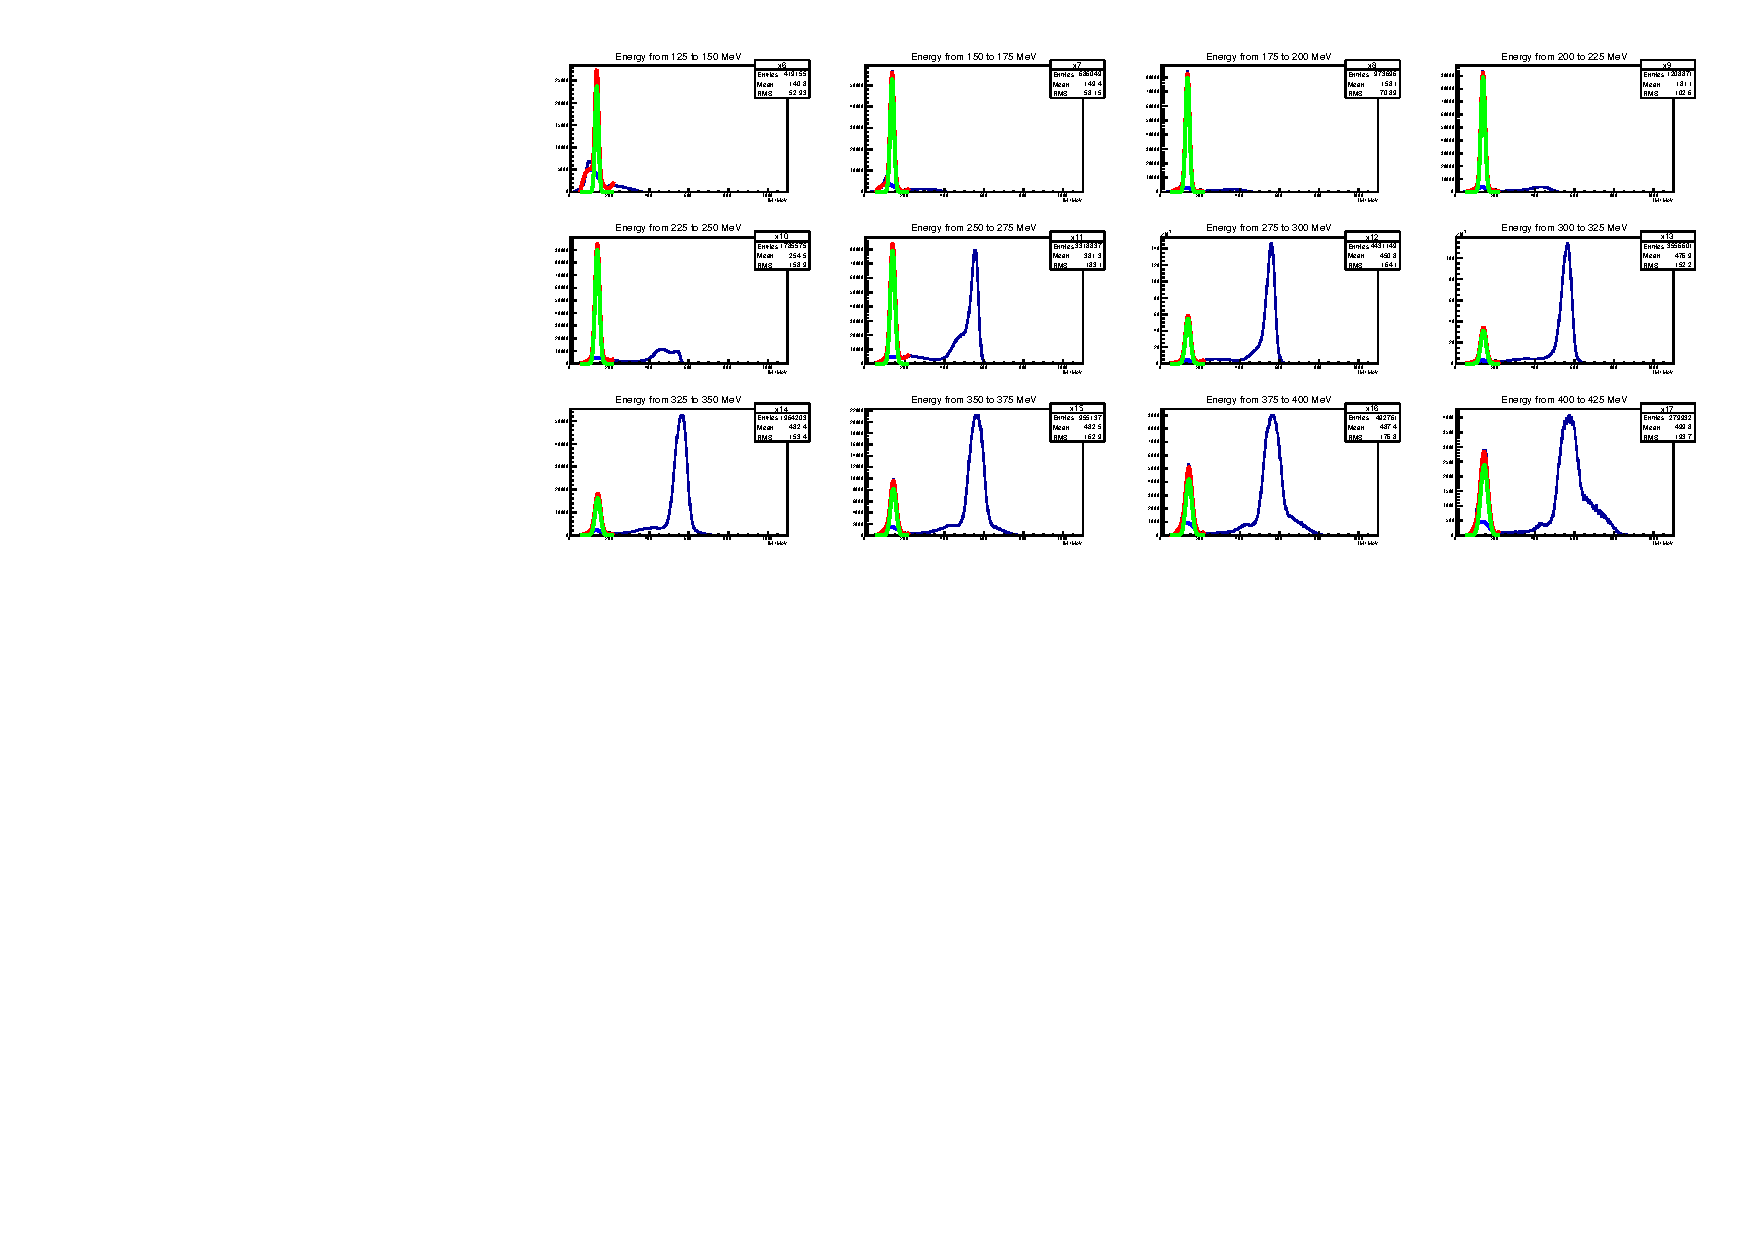
\includegraphics[width=100mm]{30DegreeCutRealDataAllFits}
		\caption{Alle Fits der Energieintervalle mit den Bedingungen, dass sich die Photonen sich energetisch ähneln und dass die detektierten Teilchen ungeladen sind. Au{\ss}erdem wurden die Detektoren am Rand vernachl\"assigt.}
		\label{fig:30-Degree-Cut-RealData-All-Fits}
	\end{center}
\end{figure}


\begin{figure}
	\begin{center}
		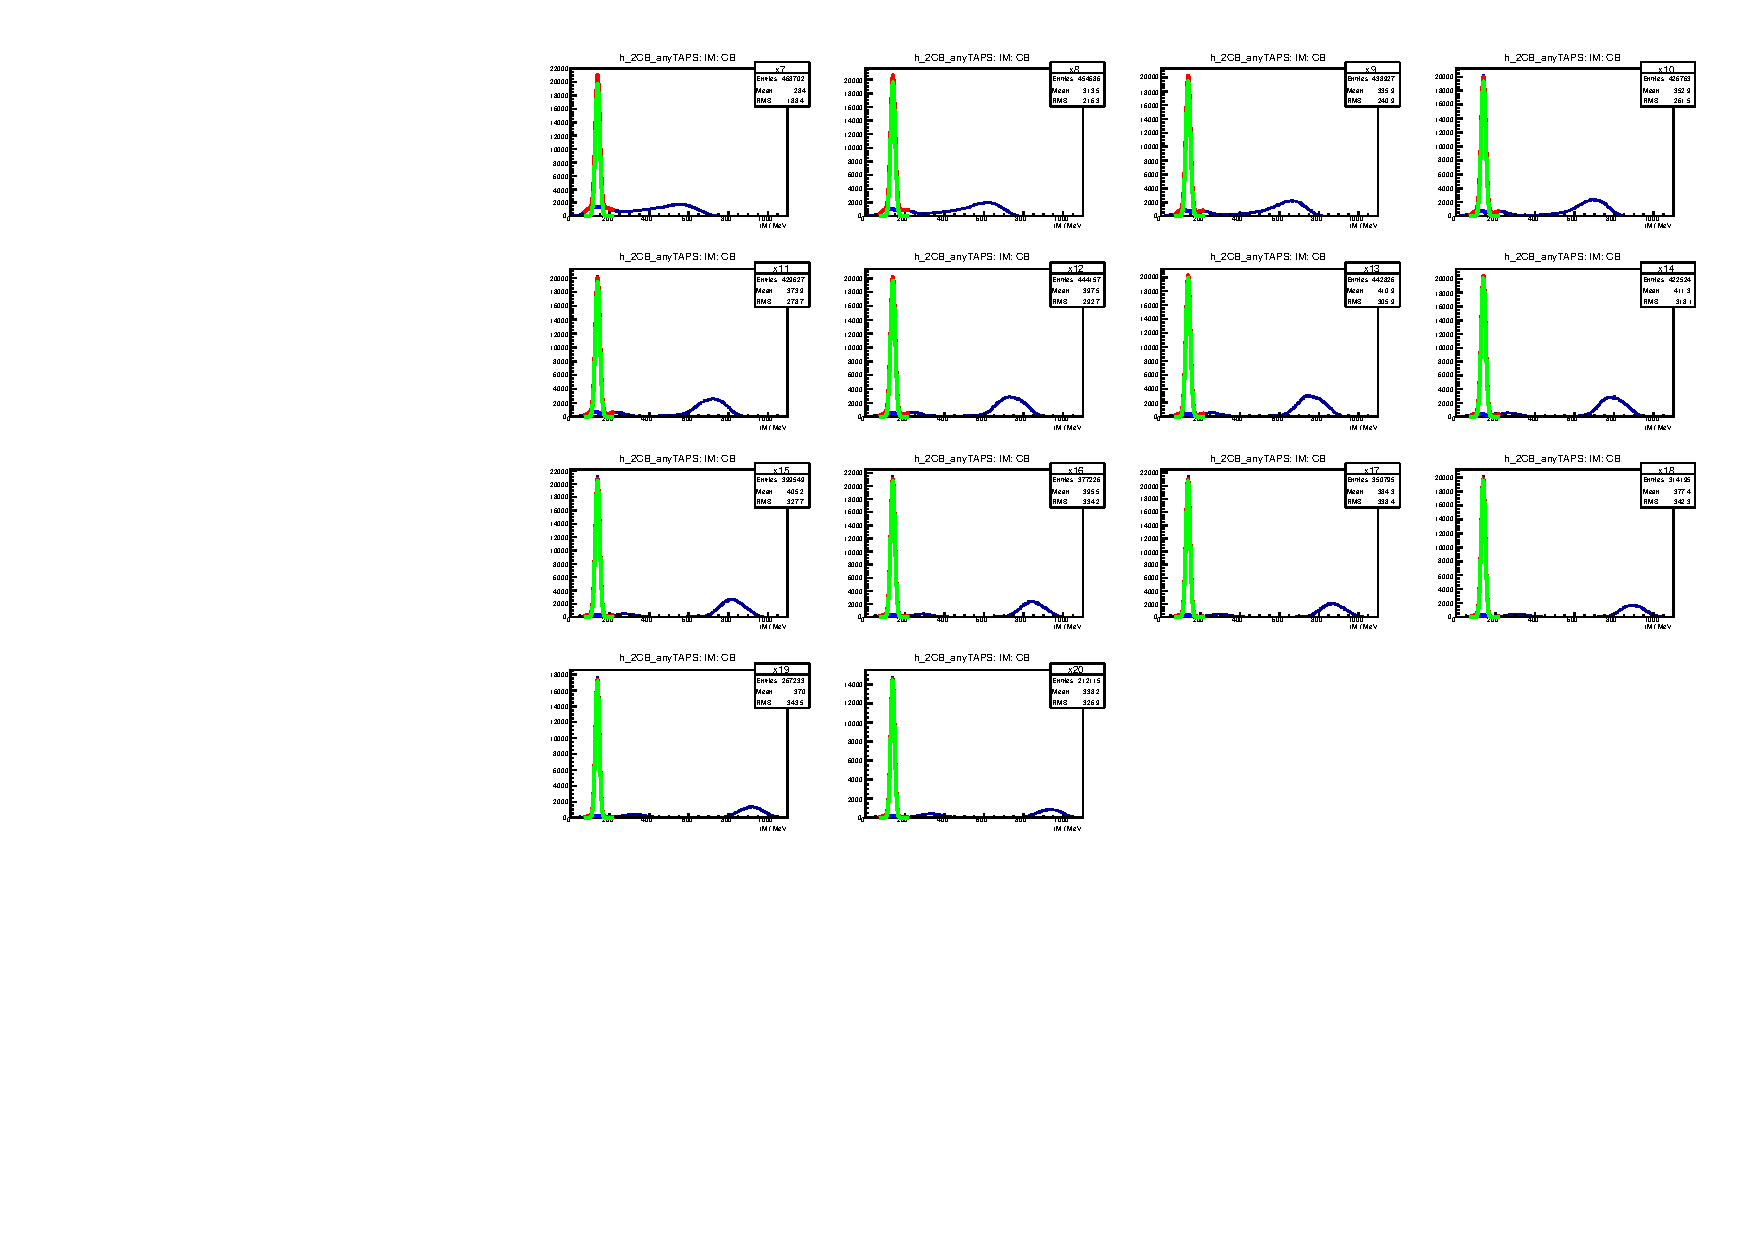
\includegraphics[width=100mm]{NoEdgeAngleAllFits1403}
		\caption{Alle Fits der Energieintervalle zur Bestimmung des $\pi^0$. Es galt keine weitere Bedingung. Daten stammen aus einer Simulation (Cocktail). Oben links ist wurde das Intervall 122 -155 MeV gefittet. Das nächste ist das Intervall von 155 - 278 MeV usw.}
	\end{center}
\end{figure}

\begin{figure}[h!]
	\begin{center}
		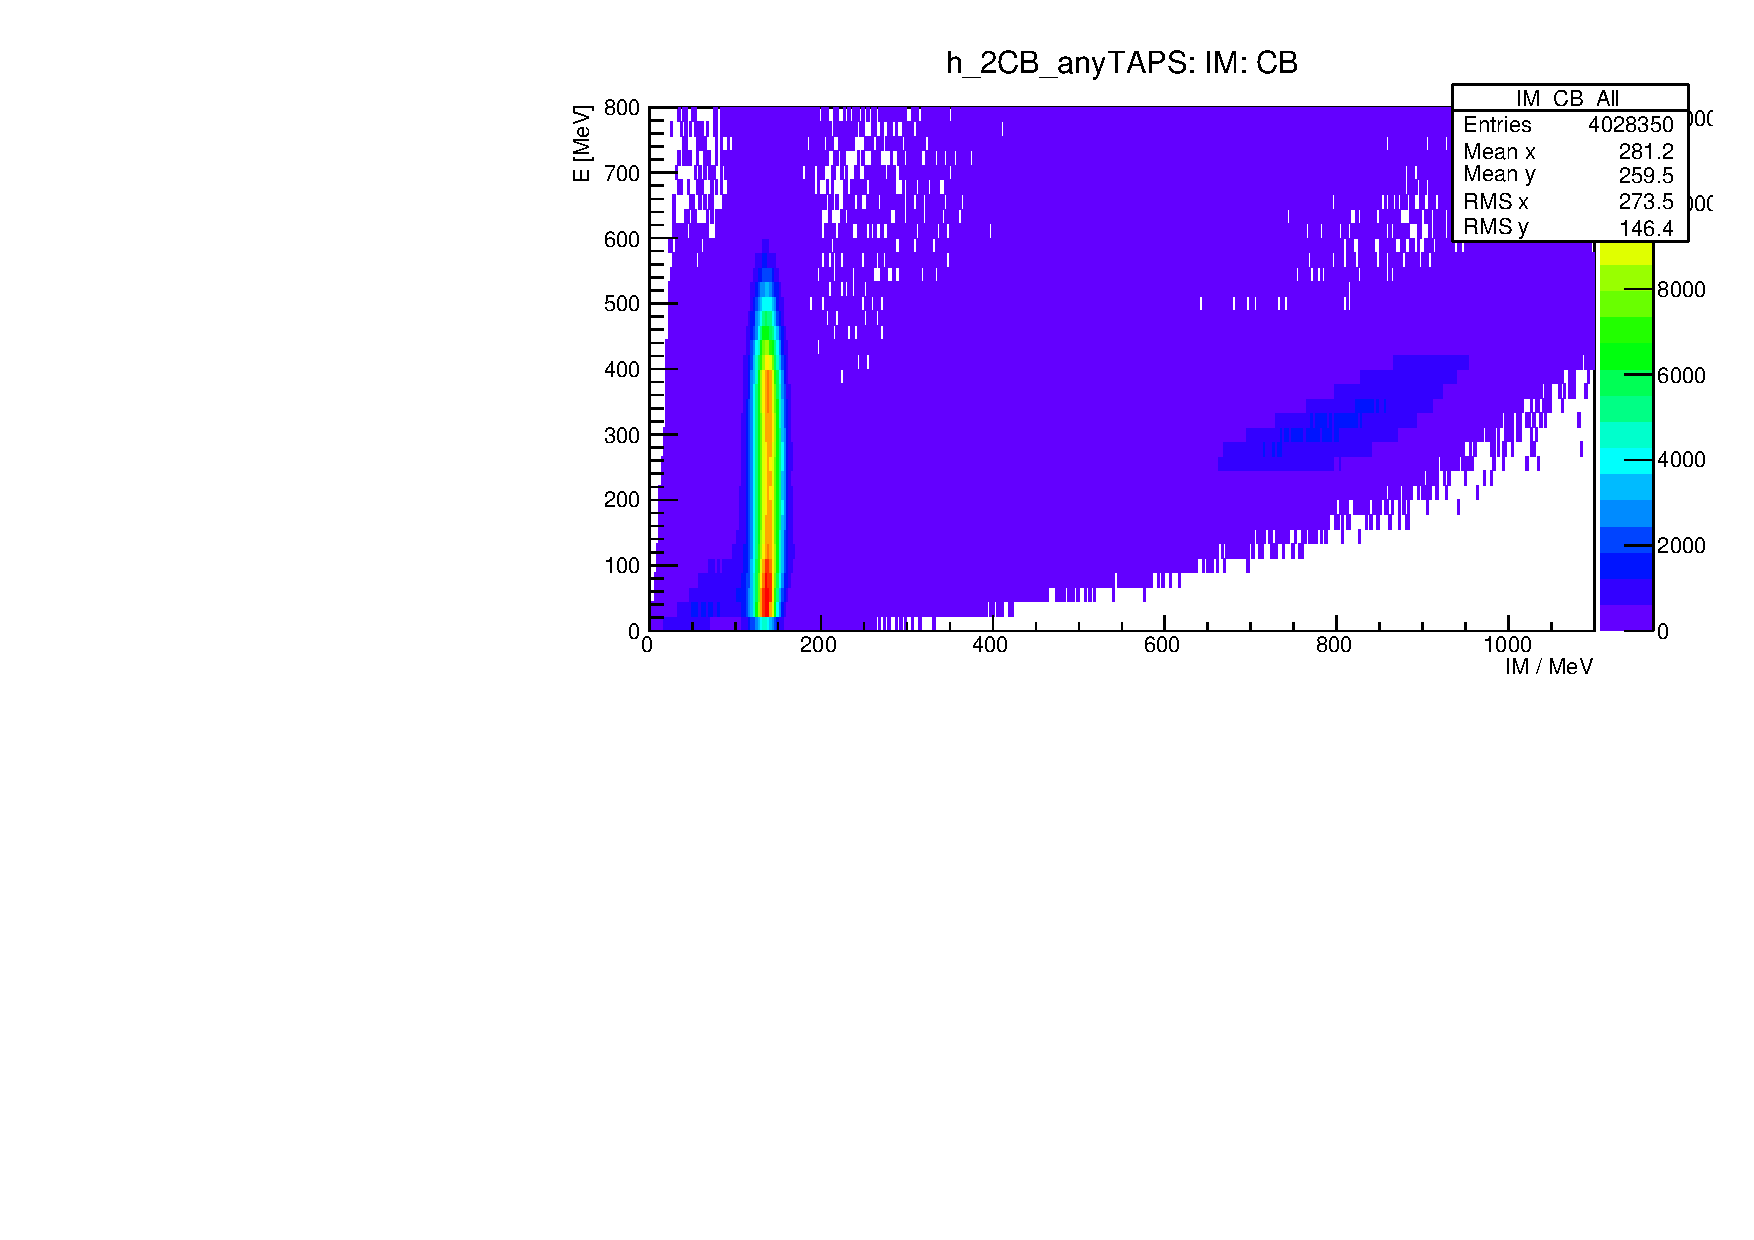
\includegraphics[width=100mm]{30DegreeEdge1403}
		\caption{Energie der Photonen gegen die errechnete invariante Masse mit der Bedingung, dass die Detektoren am Rand nicht ber\"ucksichtigt werden}
		\label{fig:Energy-Intervall-2D-Hist-30-Edge-1403}
	\end{center}
\end{figure}

\begin{figure}
	\begin{center}
		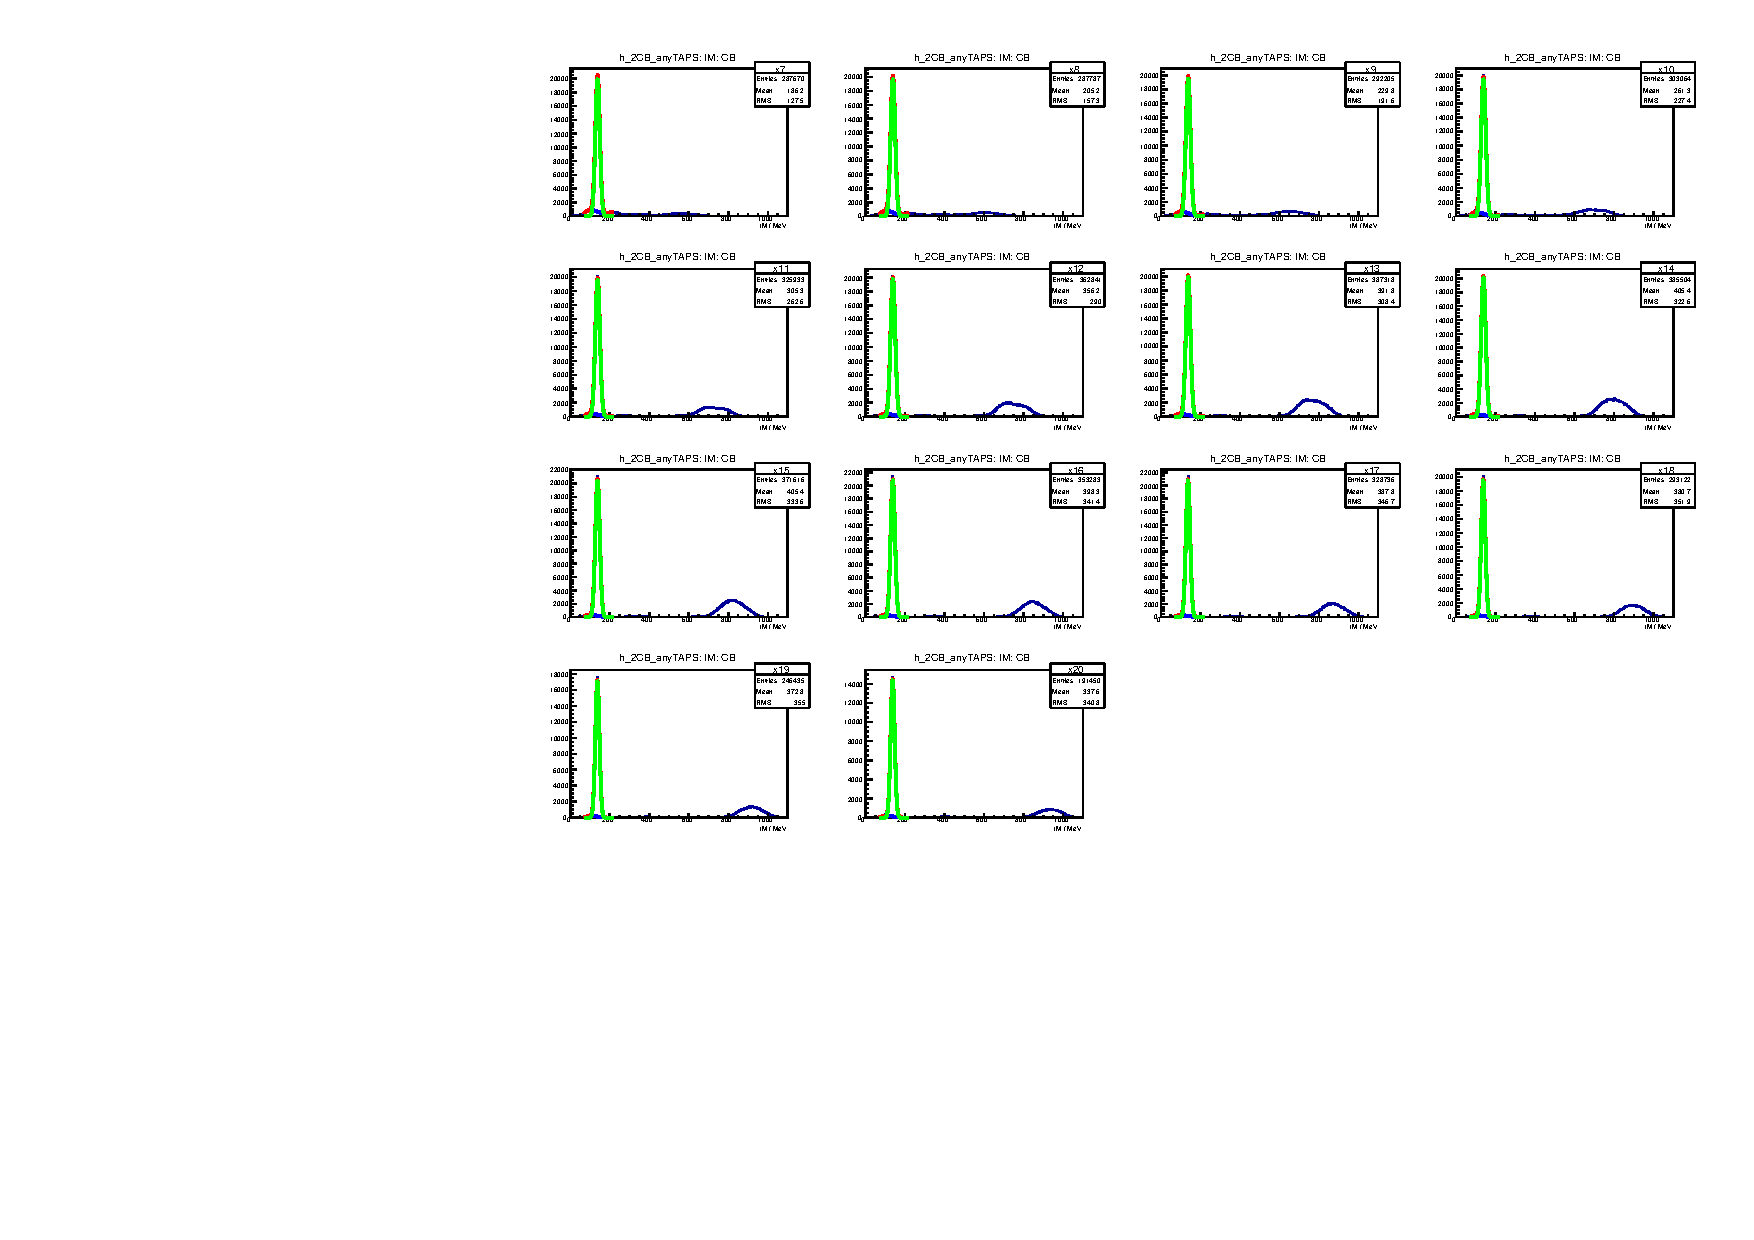
\includegraphics[width=100mm]{30DegreeEdgeAllFits}
		\caption{Alle Fits der Energieintervalle zur Bestimmung des $\pi^0$. Mit der Bedingung, dass die Detektoren am Rand vernachl\"assigt wurden. Daten stammen aus einer Simulation (Cocktail). Oben links ist wurde das Intervall 122 -155 MeV gefittet. Das nächste ist das Intervall von 155 - 278 MeV usw.}
		\label{fig:Alle-Fits-ohne-Detektoren-am-Rand}
	\end{center}
\end{figure}

\begin{figure}[h!]
	\begin{center}
		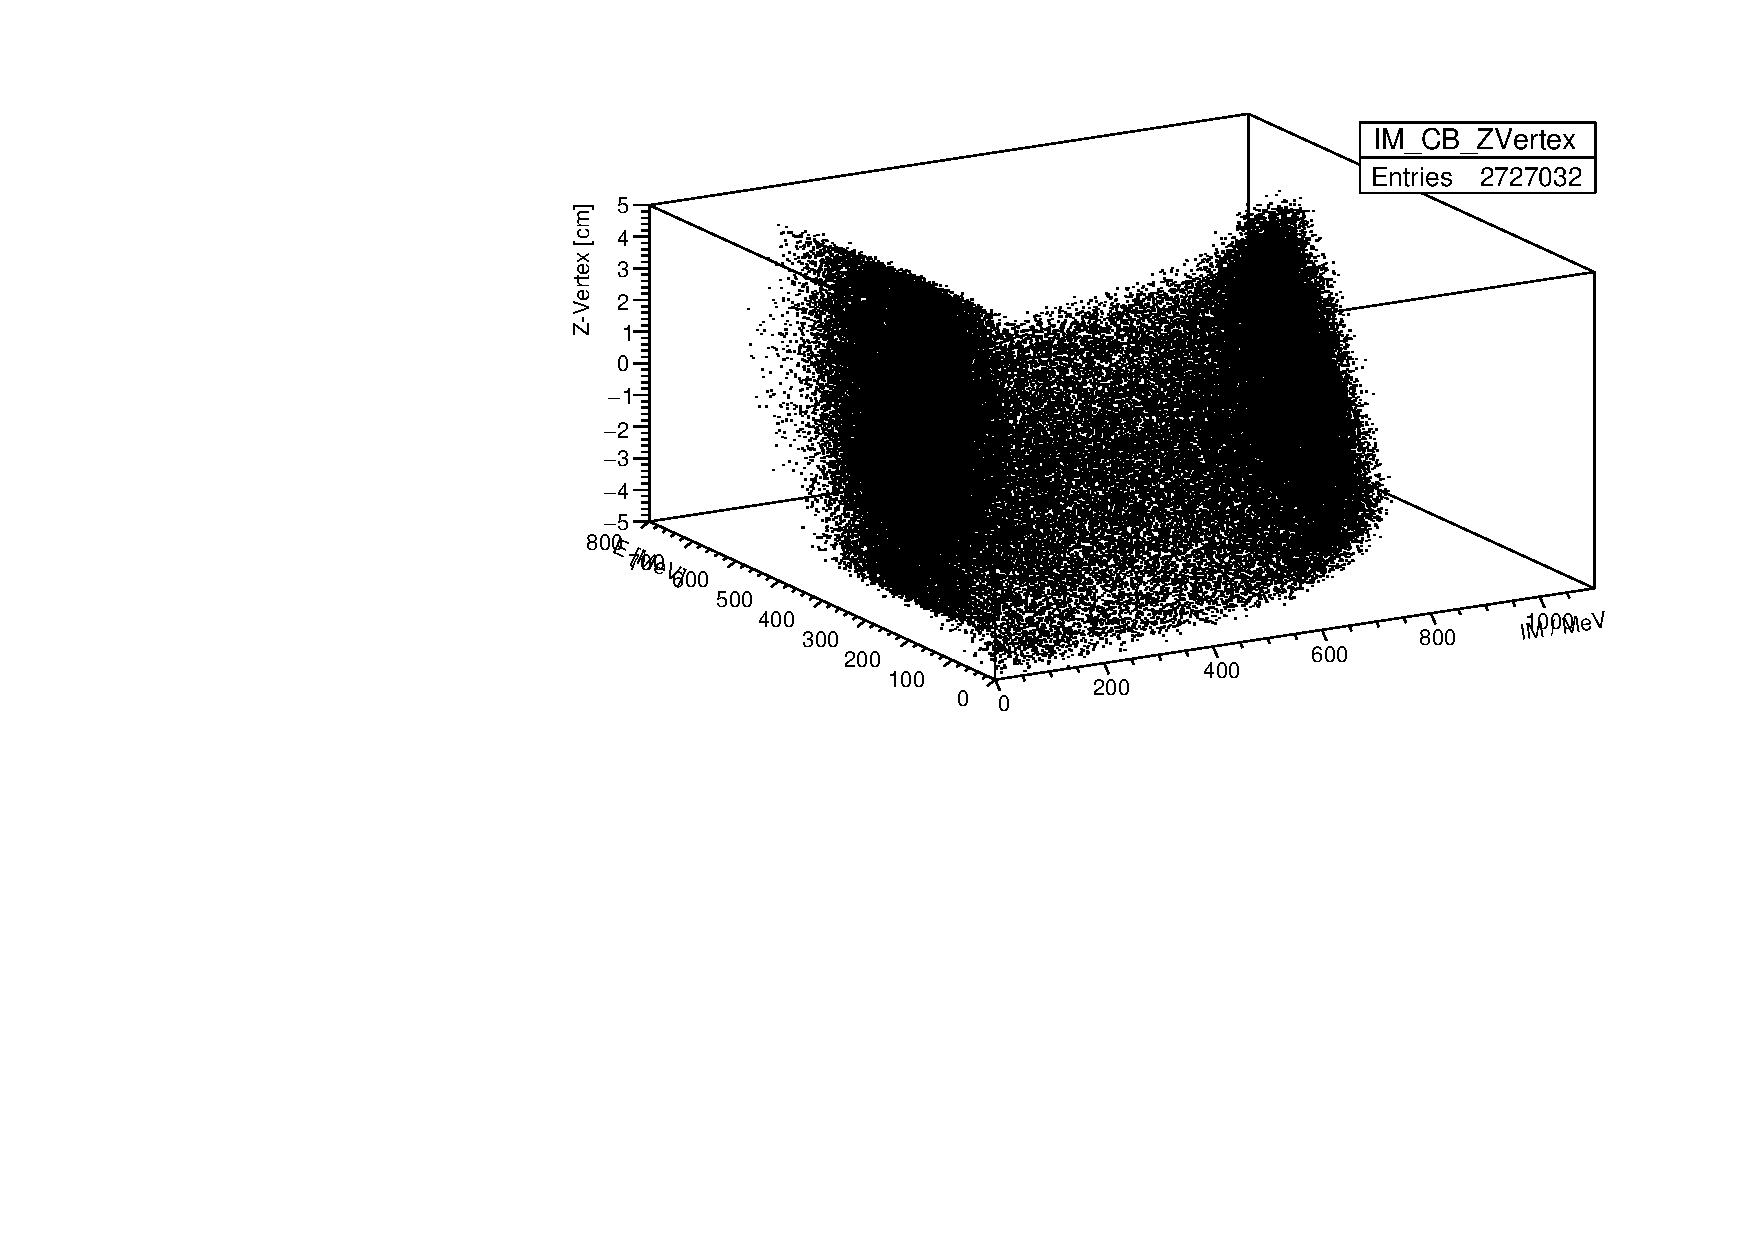
\includegraphics[width=100mm]{ZVertex3DHisto}
		\caption{Dreidmensionales Histogramm zur Untersuchung der Z-Vertex Abh\"angigkeit. Auf der z-Achse ist das Interval des Z-Vertex mit einer Breite von 1 cm aufgetragen. Auf der x-Achse ist die errechnete invariante Masse und auf der y-Achse die Energie der Photonen aufgetragen. Dieses Histogramm konnte leider nicht farbig dargestellt werden}
		\label{fig:Z-Vertex-3D-Histogramm}
	\end{center}
\end{figure}

\begin{figure}
	\begin{center}
		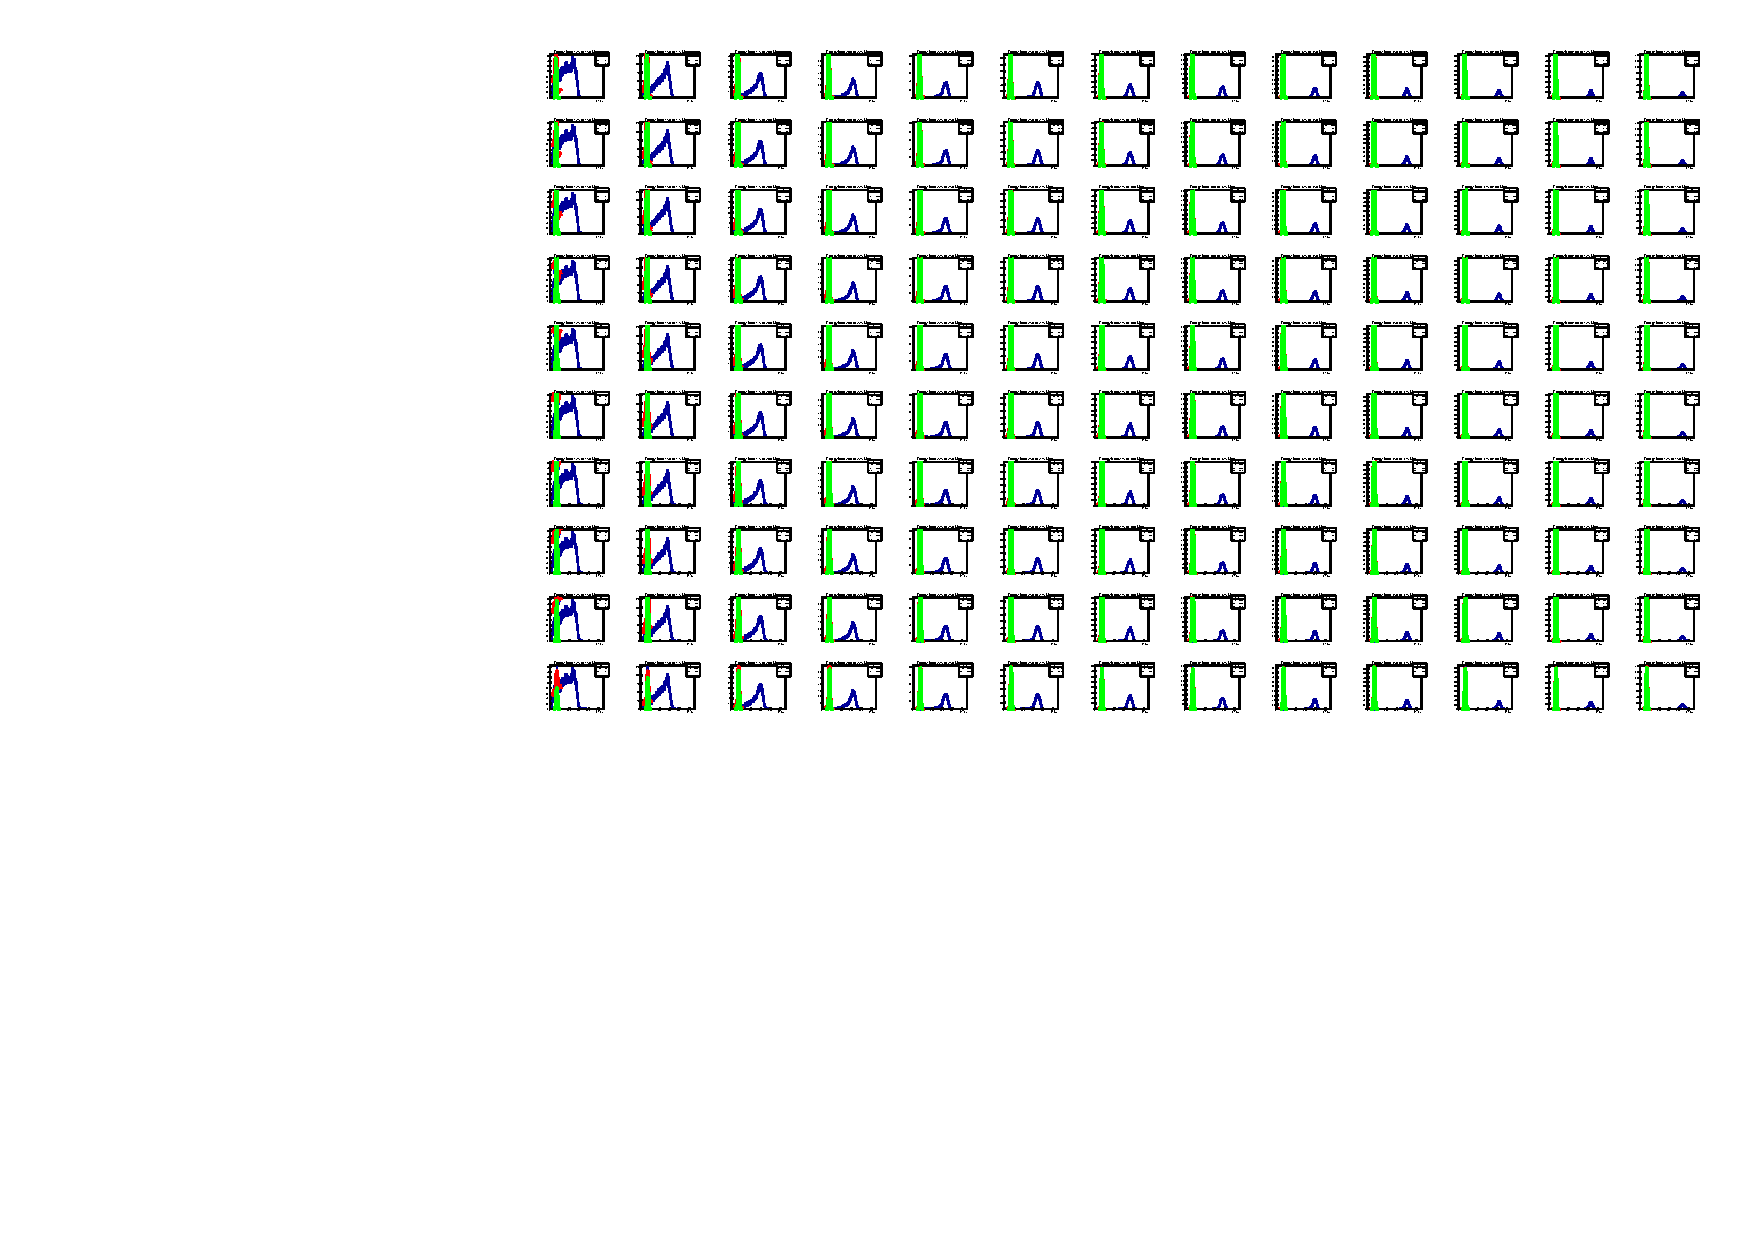
\includegraphics[width=100mm]{FullZVertexDependenceAllFits}
		\caption{Hier werden alle Fits zur Bestimmung der $\pi^0$ Position  für verschiedene Z-Vertizes aufgelistet. Die erste Zeile ist das Z-Vertex Intervall von -5 cm bis -4 cm das nächste von -4 cm bis -3 cm usw. Die Energienintervalle der Photonen sind in den Titeln der einzelnen Fits aufgetragen. Es wurden die Daten aus dem Cocktail benutzt.}
		\label{fig:Z-Vertex-All-Fits}
	\end{center}
\end{figure}

%_______________________________________________________________________________
\section{Weiterf\"uhrende Details zur Arbeit}

Manch wichtiger Teil Ihrer tats\"achlichen Arbeit ist zu technisch 
und w\"urde den Hauptteil des Textes un\"ubersichtlich machen, 
beispielsweise wenn es um die Details des Versuchsaufbaus in einer 
experimentellen Arbeit oder um den f\"ur eine numerische Auswertung 
verwendeten Algorithmus geht. Dennoch ist es sinnvoll, entsprechende 
Beschreibungen in einem Anhang Ihrer Bachelorarbeit aufzunehmen. 
Insbesondere f\"ur zuk\"unftige Arbeiten, die an Ihre Bachelorarbeit 
anschlie{\ss}en, sind dies manchmal hilfreiche Informationen.

%_______________________________________________________________________________
%\chapter{Literaturverzeichnis}

%Machen Sie genaue Angaben, so dass die verwendeten Literaturstellen 
%eindeutig identifiziert und aufgefunden werden k\"onnen.
%Bei Lehrb\"uchern \cite{Weinberg:1995mt} ist es sinnvoll, 
%den Titel anzugeben, eventuell auch die Ausgabe. Bei Artikeln in 
%Fachzeitschriften \cite{Moch:2001zr} ist es \"ublich, nur die 
%gebr\"auchlichen Abk\"urzungen f\"ur den Titel der Zeitschrift, Band, 
%Erscheinungsjahr und Seite anzugeben. Unter Umst\"anden kann es auch 
%sinnvoll sein, im Internet aufgefundene Informationsquellen anzugeben, 
%zum Beispiel f\"ur Software \cite{LoopTools} oder zu den Details von 
%Ergebnissen gro{\ss}er experimenteller Kollaborationen. Es ist 
%selbstverst\"andlich, dass Sie auch Bachelor- \cite{BA:Freund}, 
%Diplom- oder Doktorarbeiten angeben, wenn Sie diese in Ihrer eigenen 
%Arbeit verwendet haben.
%\medskip



\renewcommand{\bibname}{\bfont Literaturverzeichnis} 
\bibliographystyle{h-physrev3}
\begin{thebibliography}{99}
	
\bibitem[Un04]{Un04} Diplomarbeit von Marc Unverzagt, 2004 {\em Energie-Eichung des Crystal-Ball-Detektors am MAMI}

\bibitem[Un08]{Un08} Dissertation von Marc Unverzagt, 2008 {\em Bestimmung des Damitz-Plot-Parameters $\alpha$ für den Zerfall $ \eta \rightarrow 3\pi^{0} $ mit dem Crystal Ball am MAMI}

\bibitem[We13]{We13} Diplomarbeit von Jennifer Wettig, 2013 {\em Aufbau und Inbetriebnahme einer neuen HV-Versorgung für den Crystal Ball Detektor am MAMI}

\bibitem[KPh11G]{KPh11G} Internetseite der Kernphysik {\em Mainzer Mikrotron-Geschichte}, Internetseite \url{http://www.kernphysik.uni-mainz.de/379.php}, (Stand 04.03.2017)

\bibitem[KPh11F]{KPh11F} Internetseite der Kernphysik {\em Funktionsprinzip des MAMI}, Internetseite \url{http://www.kernphysik.uni-mainz.de/375.php}, (Stand 06.03.2017)

\bibitem[KPh04]{KPh04} Prospekt des Institut für Kernphysik Internetlink, \url{https://portal.kph.uni-mainz.de/de/information/introduction/prospekt.pdf}, (Stand: 04.03.2017)

\bibitem[KPh07]{KPh07} Pressemitteilung der KPh, \url{https://www.uni-mainz.de/presse/archiv/zope.verwaltung.uni-mainz.de/presse/mitteilung/2007/2007_10_05_phys_einweihung_mami/showArticle_dtml.html}, (Stand 06.03.2017)

\bibitem[KPh16]{KPh16} Internetseite der A2-Kollaboration {\em Reelle Photonen}
Internetseite \url{http://www.kph.uni-mainz.de/a2.php} (Stand 11.03.2017)

\bibitem[PDG16]{PDG16} Internetseite der PDG {\em Partivle Data Group} \url{http://pdg.lbl.gov/}, (Stand 20.03.2017)

\bibitem[De15]{De15} Skript \& Übungsblätter zur Vorlesung Experimentalphysik Vb WS15/16 Johannes-Gutenberg Universi\"at Mainz, Prof. Denig \url{https://reader.uni-mainz.de/WiSe2015-16/08-128-055-00/_layouts/15/start.aspx#/Lists/DocumentLib/Forms/AllItems.aspx?RootFolder=}, (Stand: 14.03.2017)

\bibitem[NBI15]{NBI15} Einf\"urung in die Programmierung mit Root von Manuel Calderon de la Barca Sanchez \url{http://www.nbi.dk/~petersen/Teaching/Stat2015/PythonRootIntro/ROOT_TipsAndTricks.pdf} (Stand: 27.03.2017)








%\cite{BA:Freund}
\bibitem{BA:Freund}
  B.~Freund Nummer eins, 
  Bachelorarbeit, Johannes Gutenberg-Universit\"at Mainz, 2012.

\end{thebibliography}

%_______________________________________________________________________________
\chapter{Danksagung}

... an wen auch immer. Denken Sie an Ihre Freundinnen und Freunde, 
Familie, Lehrer, Berater und Kollegen.

\end{appendix}


\end{document}  
        
        